%%***********************************************
%% Plantilla para TFG.
%% Escuela Técnica Superior de Ingenieros Informáticos. UPM.
%%***********************************************

%%-----------------------------------------------
%% Importar Preámbulo:
% -*-coding: utf-8 -*-
%%***********************************************
%% Plantilla para TFG.
%% Escuela Técnica Superior de Ingenieros Informáticos. UPM.
%%***********************************************
%% Preámbulo del documento.
%%***********************************************
\documentclass[a4paper,11pt,openany]{book}
\usepackage[utf8]{inputenc}
\usepackage[T1]{fontenc}
\usepackage[english,spanish,es-lcroman]{babel}
\usepackage{bookman}
\decimalpoint
\usepackage{graphicx}
\usepackage{amsfonts,amsgen,amsmath,amssymb}
\usepackage[top=3cm, bottom=3cm, right=2.54cm, left=2.54cm]{geometry}
\usepackage{afterpage}
\usepackage{colortbl,longtable}
\usepackage[
  pdftex,
  pdfauthor={Miguel Alonso, Carlos},
  pdftitle={Trabajo de Fin de Grado},
  pdfborder={0 0 0}
]{hyperref}
\usepackage{pdfpages}
\usepackage{url}
\usepackage[stable]{footmisc}
\usepackage{parskip} % para separar párrafos con espacio.

\usepackage{lscape}
\usepackage{pgfgantt}

% --- BIBLIOGRAPHY ---
\usepackage[
  backend=biber,
  style=numeric,
  sorting=none
]{biblatex}
\bibliography{bibliography}
\usepackage{csquotes}
% --- BIBLIOGRAPHY ---

\usepackage{float}
\usepackage{subfigure}

%%-----------------------------------------------
\usepackage{fancyhdr}
\pagestyle{fancy}
\fancyhf{}
\fancyhead[LO]{\leftmark}
\fancyhead[RE]{\rightmark}
\setlength{\headheight}{1.5\headheight}
\cfoot{\thepage}

\addto\captionsspanish{ \renewcommand{\contentsname}
  {Índice general} }
\setcounter{tocdepth}{4}
\setcounter{secnumdepth}{4}

\renewcommand{\chaptermark}[1]{\markboth{\textbf{#1}}{}}
\renewcommand{\sectionmark}[1]{\markright{\textbf{\thesection. #1}}}
\newcommand{\HRule}{\rule{\linewidth}{0.5mm}}
\newcommand{\bigrule}{\titlerule[0.5mm]}

\usepackage{appendix}
\renewcommand{\appendixname}{Anexos}
\renewcommand{\appendixtocname}{Anexos}
\renewcommand{\appendixpagename}{}
%%-----------------------------------------------
%% Páginas en blanco sin cabecera:
%%-----------------------------------------------
\usepackage{dcolumn}
\newcolumntype{.}{D{.}{\esperiod}{-1}}
\makeatletter
\addto\shorthandsspanish{\let\esperiod\es@period@code}

\def\clearpage{
  \ifvmode
  \ifnum \@dbltopnum =\m@ne
  \ifdim \pagetotal <\topskip
  \hbox{}
  \fi
  \fi
  \fi
  \newpage
  \thispagestyle{empty}
  \write\m@ne{}
  \vbox{}
  \penalty -\@Mi
}
\makeatother
%%-----------------------------------------------
%% Estilos código de lenguajes: Consola, C, C++ y Python
%%-----------------------------------------------
\usepackage{color}

\definecolor{gray97}{gray}{.97}
\definecolor{gray75}{gray}{.75}
\definecolor{gray45}{gray}{.45}

\usepackage{listings}
\lstset{ frame=Ltb,
  framerule=0pt,
  aboveskip=0.5cm,
  framextopmargin=3pt,
  framexbottommargin=3pt,
  framexleftmargin=0.4cm,
  framesep=0pt,
  rulesep=.0pt,
  backgroundcolor=\color{gray97},
  rulesepcolor=\color{black},
  %
  stringstyle=\ttfamily,
  showstringspaces = false,
  basicstyle=\scriptsize\ttfamily,
  commentstyle=\color{gray45},
  keywordstyle=\bfseries,
  %
  numbers=left,
  numbersep=6pt,
  numberstyle=\tiny,
  numberfirstline = false,
  breaklines=true,
}
\lstnewenvironment{listing}[1][]
                  {\lstset{#1}\pagebreak[0]}{\pagebreak[0]}
                    \lstdefinestyle{consola}{
                                    basicstyle=\scriptsize\bf\ttfamily,
                                    backgroundcolor=\color{gray97}}
                    \lstdefinestyle{C}{
                                    basicstyle=\scriptsize,
                                    frame=single,
                                    language=C,
                                    numbers=left}
                    \lstdefinestyle{C++}{
                                    basicstyle=\small,
                                    frame=single,
                                    backgroundcolor=\color{gray75},
                                    language=C++,
                                    numbers=left}
                    \lstdefinestyle{Java}{
                                    basicstyle=\small,
                                    frame=single,
                                    backgroundcolor=\color{gray75},
                                    language=Java,
                                    numbers=left}
                                \makeatother


%%-----------------------------------------------
%% Cargar datos relativos al TFG:
%% (actualizar estos datos en secciones/_DatosTFG.tex)
%***********************************************
%% Plantilla para TFG.
%% Escuela Técnica Superior de Ingenieros Informáticos. UPM.
%%***********************************************
%% Información requerida para completar la portada.
%%*********************************************** 

%% Escribe Nombre y Apellidos del autor del trabajo:
\newcommand{\NombreAutor}{ Carlos Miguel Alonso }

%% Escribe el Grado: 
\newcommand{\Grado}{ Ingeniería Informática }

%% Escribe el Título del Trabajo:
\newcommand{\TituloTFG}{ Mejora de un Sistema de Auto-escalado para Sistemas Distribuidos } 

%% Escribe Nombre y Apellidos del Tutor del trabajo: 
\newcommand{\NombreTutor}{ Victor Rampérez Martín } 

% Escribe el Departamento al que pertenece el Tutor:
\newcommand{\Departamento}{ Departamento de Lenguajes, Sistemas Informáticos e Ingeniería del Software }

% Escribe la fecha de lectura, en formato: Mes - Año
\newcommand{\Fecha}{ Febrero - 2022 }
%%***********************************************


%%-----------------------------------------------
%% Documento:
\begin{document}

\renewcommand\listfigurename{Índice de Figuras}
\renewcommand\listtablename{Índice de Tablas}
\renewcommand\lstlistlistingname{Índice de Listings}

%%***********************************************
%% Plantilla para TFG.
%% Escuela Técnica Superior de Ingenieros Informáticos. UPM.
%%***********************************************
%% Portada.
%%***********************************************
\begin{titlepage}

  \begin{minipage}{0.15\linewidth}
    \hspace*{-2.5cm}
    \noindent
    
\includegraphics[scale=0.5]{./include/EscUpm.png} \qquad\qquad
  \end{minipage}
  \begin{minipage}{0.7\linewidth}
    \begin{center}
      \huge{ Universidad Politécnica\\de Madrid }\\
      \vspace*{0.5cm}
      \Large{\textbf{Escuela Técnica Superior de \\
          Ingenieros Informáticos}}
    \end{center}
  \end{minipage}
  \begin{minipage}{0.2\linewidth}
    
\includegraphics[scale=0.5]{./include/FacInformatica.png}
  \end{minipage}

  \vspace*{1cm}
  \begin{center}
    \Large{Grado en  \Grado{} }
  \end{center}

  \vspace*{1cm}
  \begin{center}
    \huge{ Trabajo Fin de Grado}% \\ \textit{Plan de Trabajo}}
  \end{center}

  \vspace*{0.5cm}
  \begin{center}
    \huge\bfseries {  \TituloTFG{} }
  \end{center}

  \vspace*{5cm}

  \noindent
  \large{Autor: \NombreAutor{} }\\
  \large{Tutor: \NombreTutor{} }


  \vspace*{4cm}
  \begin{center}
    Madrid, \Fecha
  \end{center}

 %% %%--------------------------------
  \newpage
  \thispagestyle{empty}
  %%--------------------------------
  \noindent
  Este Trabajo Fin de Grado se ha depositado en la ETSI Informáticos de la Universidad Politécnica de Madrid para su defensa.

  \vspace*{4cm}
  \noindent
  \textit{Trabajo Fin de Grado}\\
  \textit{Grado en} \Grado{}
  
  \textit{Título:} \TituloTFG{}

  \Fecha

  \vspace*{3cm}

  \noindent
  \begin{tabular}{ll}
     \textit{Autor:} & \NombreAutor{}  \\
     \textit{Tutor:} & \NombreTutor{}  \\
     & \Departamento{} \\
     & Escuela Técnica Superior de Ingenieros Informáticos\\
     & Universidad Politécnica de Madrid
  \end{tabular}

\end{titlepage}


%%-----------------------------------------------
%% Numeración romana:
\frontmatter

%%-----------------------------------------------
% \chapter*{Resumen} \label{chp:abstract}

Uno de los principales pilares de la computación en la nube es la elasticidad, 
es decir, la capacidad de ajustar los recursos necesarios de forma automática 
para cubrir la demanda en cada instante. Los sistemas de auto-escalado son los 
encargados de dotar de elasticidad a los sistemas escalables. 
Dichos sistemas de auto-escalado están recibiendo gran atención en los 
últimos años debido a la expansión de las arquitecturas basadas en
micro-servicios (e.g. Kubernetes y Docker) y al auge de la computación en la nube.

En el contexto de este proyecto, se está desarrollando un sistema de auto-escalado que combina las 
técnicas de auto-escalado reactivas y predictivas mediante la aplicación de 
modelos estadísticos.

Este Trabajo de Fin de Grado aborda la mejora del auto-escalado de sistemas 
distribuidos por medio del estudio del comportamiento de E-SilboPs bajo una carga
de trabajo real a través de la obtención y monitorización de las métricas de 
rendimiento relevantes.

Con este fin, se ha llevado a cabo una búsqueda de una carga de trabajo que se 
haya usado en un contexto de uso real. La carga escogida, procedente del sistema PADRES, un sistema 
publicador/subscriptor basado en contenido ampliamente usado en literatura, ha
de ser traducida al formato de E-SilboPS. Para esto, se ha diseñado e implementado
un generador de cargas de trabajo reales, que traducirá los eventos de dicha carga,
manteniendo el contexto y contenido de cada uno de ellos (usuario,
parámetros de las subscripciones y publicaciones, etc.).

Una vez traducida la carga de trabajo, para medir el rendimiento del sistema
con esta, se han diseñado e implementado diferentes pruebas para obtener estas
métricas de rendimiento, lo que permite identificar la saturación y comportamiento
del sistema. Esto ha permitido la generación de otras cargas basadas en la real para
llevar al sistema a situaciones especiales y medir su respuesta de forma más
detallada.

A continuación, se han diseñado e implementado diferentes modelos predictivos basados
en Machine-Learning y Deep-Learning, que se aplicarán a los resultados de las pruebas
realizadas, con el objetivo de predecir el comportamiento del sistema y así
aplicar estas predicciones al sistema de auto-escalado.

Los resultados obtenidos en este Trabajo de Fin de Grado muestran el correcto
funcionamiento del generador de cargas de trabajo, al haber traducido la carga
de PADRES de forma satisfactoria; y la utilidad de dicha carga, al comprobar
que E-SilboPS llega a saturar parcialmente, posibilitando la aplicación de los
modelos predictivos para predecir futuras situaciones de saturación.

\textbf{Palabras Clave:} Auto-escalado, Sistemas Distribuidos, Cloud, Modelos Estadísticos.

%%%%%%%%%%%%%%%%%%%%%%%%%%%%%%%%%%%%%%%%%%%%%%%%%%%%%%%%%%%%%%%%%%%%%%%%%%%%%%%%
%%%%%%%%%%%%%%%%%%%%%%%%%%%%%%%%%%%%%%%%%%%%%%%%%%%%%%%%%%%%%%%%%%%%%%%%%%%%%%%%

%%--------------
\newpage
%%--------------

%%%%%%%%%%%%%%%%%%%%%%%%%%%%%%%%%%%%%%%%%%%%%%%%%%%%%%%%%%%%%%%%%%%%%%%%%%%%%%%%
%%%%%%%%%%%%%%%%%%%%%%%%%%%%%%%%%%%%%%%%%%%%%%%%%%%%%%%%%%%%%%%%%%%%%%%%%%%%%%%%

\chapter*{Abstract}

One of the main pillars of cloud computing is elasticity, i.e. the ability to 
automatically adjust the resources needed to meet the demand at any given time.
Auto-scaling systems are responsible of providing elasticity to scalable systems.
This auto-scaling systems are getting increasing attention in recent years thanks 
to the growth of micro-services based architectures, e.g. Kubernetes and Docker, 
and the rise on popularity of cloud computing.

In the context of this project, an auto-scaler system is being developed, that
combines both reactive and predictive auto-scaling techniques by applying 
statistical models.

This Trabajo de Fin de Grado addresses the improvement of the auto-scaling of 
distributed systems by studying the behaviour of E-SilboPS under a real-world workload,
obtaining the relevant performance measurements.

To this end, a search has been carried out for a workload that has been used in a 
real-world context. This workload must be compatible with the E-SilboPS system, 
analysing its content to obtain statistical data, and verifying  the completeness and 
compatibility of this workload data.

The chosen real-world workload, extracted from PADRES, a content-based 
publish/subscribe system widely used on literature; must be translated to the E-SilboPS
format. To achieve this, a real workload generator has been designed and implemented, 
that performs this translation by interpreting each event and its content, and 
transforming it to the E-SilboPS syntax, keeping its original context (user, 
subscription and publications parameters, etc.).

With the workload already translated, to test the system performance using it, 
different tests have been developed to obtain its system performance metrics, allowing
detection of situations in which the system saturates. This allowed the creation of
other workloads, based on the real-world one, that tests the system on special
situations and measure the system response in more detail.


Once the system has been tested, different predictive models have been designed and
implemented, based on Machine-Learning and Deep-Learning, that will be applied to the 
results of the tests carried out, in order to predict the behaviour of the system and 
then apply these predictions to the auto-scaling system.

The results obtained of this Trabajo de Fin de Grado reflect the real workload generator 
working correctly, since it translated the PADRES real-world workload; and the usefulness of said
workload through verifying that E-SilboPS partially saturates, which opens the door
to the possibility of implementing improvements on FLAS if new predictive models are applied.

\textbf{Keywords:} Auto-scaling, Distributed Systems, Cloud, Statistical Models.


%%%%%%%%%%%%%%%%%%%%%%%%%%%%%%%%%%%%%%%%%%%%%%%%%%%%%%%%%%%
%% Final del resumen. 
%%%%%%%%%%%%%%%%%%%%%%%%%%%%%%%%%%%%%%%%%%%%%%%%%%%%%%%%%%%R
\tableofcontents


\lstlistoflistings
\listoftables
\listoffigures

%%-----------------------------------------------
%% Numeración arábiga:
\mainmatter

%%-----------------------------------------------
\chapter*{Resumen} \label{chp:abstract}

Uno de los principales pilares de la computación en la nube es la elasticidad, 
es decir, la capacidad de ajustar los recursos necesarios de forma automática 
para cubrir la demanda en cada instante. Los sistemas de auto-escalado son los 
encargados de dotar de elasticidad a los sistemas escalables. 
Dichos sistemas de auto-escalado están recibiendo gran atención en los 
últimos años debido a la expansión de las arquitecturas basadas en
micro-servicios (e.g. Kubernetes y Docker) y al auge de la computación en la nube.

En el contexto de este proyecto, se está desarrollando un sistema de auto-escalado que combina las 
técnicas de auto-escalado reactivas y predictivas mediante la aplicación de 
modelos estadísticos.

Este Trabajo de Fin de Grado aborda la mejora del auto-escalado de sistemas 
distribuidos por medio del estudio del comportamiento de E-SilboPs bajo una carga
de trabajo real a través de la obtención y monitorización de las métricas de 
rendimiento relevantes.

Con este fin, se ha llevado a cabo una búsqueda de una carga de trabajo que se 
haya usado en un contexto de uso real. La carga escogida, procedente del sistema PADRES, un sistema 
publicador/subscriptor basado en contenido ampliamente usado en literatura, ha
de ser traducida al formato de E-SilboPS. Para esto, se ha diseñado e implementado
un generador de cargas de trabajo reales, que traducirá los eventos de dicha carga,
manteniendo el contexto y contenido de cada uno de ellos (usuario,
parámetros de las subscripciones y publicaciones, etc.).

Una vez traducida la carga de trabajo, para medir el rendimiento del sistema
con esta, se han diseñado e implementado diferentes pruebas para obtener estas
métricas de rendimiento, lo que permite identificar la saturación y comportamiento
del sistema. Esto ha permitido la generación de otras cargas basadas en la real para
llevar al sistema a situaciones especiales y medir su respuesta de forma más
detallada.

A continuación, se han diseñado e implementado diferentes modelos predictivos basados
en Machine-Learning y Deep-Learning, que se aplicarán a los resultados de las pruebas
realizadas, con el objetivo de predecir el comportamiento del sistema y así
aplicar estas predicciones al sistema de auto-escalado.

Los resultados obtenidos en este Trabajo de Fin de Grado muestran el correcto
funcionamiento del generador de cargas de trabajo, al haber traducido la carga
de PADRES de forma satisfactoria; y la utilidad de dicha carga, al comprobar
que E-SilboPS llega a saturar parcialmente, posibilitando la aplicación de los
modelos predictivos para predecir futuras situaciones de saturación.

\textbf{Palabras Clave:} Auto-escalado, Sistemas Distribuidos, Cloud, Modelos Estadísticos.

%%%%%%%%%%%%%%%%%%%%%%%%%%%%%%%%%%%%%%%%%%%%%%%%%%%%%%%%%%%%%%%%%%%%%%%%%%%%%%%%
%%%%%%%%%%%%%%%%%%%%%%%%%%%%%%%%%%%%%%%%%%%%%%%%%%%%%%%%%%%%%%%%%%%%%%%%%%%%%%%%

%%--------------
\newpage
%%--------------

%%%%%%%%%%%%%%%%%%%%%%%%%%%%%%%%%%%%%%%%%%%%%%%%%%%%%%%%%%%%%%%%%%%%%%%%%%%%%%%%
%%%%%%%%%%%%%%%%%%%%%%%%%%%%%%%%%%%%%%%%%%%%%%%%%%%%%%%%%%%%%%%%%%%%%%%%%%%%%%%%

\chapter*{Abstract}

One of the main pillars of cloud computing is elasticity, i.e. the ability to 
automatically adjust the resources needed to meet the demand at any given time.
Auto-scaling systems are responsible of providing elasticity to scalable systems.
This auto-scaling systems are getting increasing attention in recent years thanks 
to the growth of micro-services based architectures, e.g. Kubernetes and Docker, 
and the rise on popularity of cloud computing.

In the context of this project, an auto-scaler system is being developed, that
combines both reactive and predictive auto-scaling techniques by applying 
statistical models.

This Trabajo de Fin de Grado addresses the improvement of the auto-scaling of 
distributed systems by studying the behaviour of E-SilboPS under a real-world workload,
obtaining the relevant performance measurements.

To this end, a search has been carried out for a workload that has been used in a 
real-world context. This workload must be compatible with the E-SilboPS system, 
analysing its content to obtain statistical data, and verifying  the completeness and 
compatibility of this workload data.

The chosen real-world workload, extracted from PADRES, a content-based 
publish/subscribe system widely used on literature; must be translated to the E-SilboPS
format. To achieve this, a real workload generator has been designed and implemented, 
that performs this translation by interpreting each event and its content, and 
transforming it to the E-SilboPS syntax, keeping its original context (user, 
subscription and publications parameters, etc.).

With the workload already translated, to test the system performance using it, 
different tests have been developed to obtain its system performance metrics, allowing
detection of situations in which the system saturates. This allowed the creation of
other workloads, based on the real-world one, that tests the system on special
situations and measure the system response in more detail.


Once the system has been tested, different predictive models have been designed and
implemented, based on Machine-Learning and Deep-Learning, that will be applied to the 
results of the tests carried out, in order to predict the behaviour of the system and 
then apply these predictions to the auto-scaling system.

The results obtained of this Trabajo de Fin de Grado reflect the real workload generator 
working correctly, since it translated the PADRES real-world workload; and the usefulness of said
workload through verifying that E-SilboPS partially saturates, which opens the door
to the possibility of implementing improvements on FLAS if new predictive models are applied.

\textbf{Keywords:} Auto-scaling, Distributed Systems, Cloud, Statistical Models.


%%%%%%%%%%%%%%%%%%%%%%%%%%%%%%%%%%%%%%%%%%%%%%%%%%%%%%%%%%%
%% Final del resumen. 
%%%%%%%%%%%%%%%%%%%%%%%%%%%%%%%%%%%%%%%%%%%%%%%%%%%%%%%%%%%R
\chapter{Introducción} \label{chp:intro}

En este capítulo se presentan y explican la motivación, el contexto, los objetivos
específicos del trabajo realizado y la estructura de este documento, con la 
intención de proporcionar una visión general del mismo.

%%%%%%%%%%%%%%%%%%%%%%%%%%%%%%%%%%%%%%%%%%%%%%%%%%%%%%%%%%%%%%%%%%%%%%%%%%%%%%%%
%%%%%%%%%%%%%%%%%%%%%%%%%%%%%%%%%%%%%%%%%%%%%%%%%%%%%%%%%%%%%%%%%%%%%%%%%%%%%%%%

\section{Motivación del proyecto} \label{sct:intro_motivacion}

% - Digitalización
% - Paradigmas como el IoT, Smart Cities, ...
% - Sistemas dirigidos por eventos que dan soporte a estos paradigmas
% - Sistemas, como los pub/sub, se apoyan en el cloud computing para...
% - Cloud computing ofrece la ventaja de la elasticidad (explicar)
% - Elasticidad y al necesidad de la misma para nuestro tipo de sistema

En los últimos años se ha producido un incremento significativo en la 
digitalización de numerosos aspectos de la vida cotidiana de las personas como 
consecuencia de la popularización de nuevos paradigmas tecnológicos como las 
Smart Cities o el Internet of Things\footnote{Dispositivos físicos con sensores y 
software que conectan e intercambian datos con otros dispositivos y sistemas a 
través de Internet} (o IoT, por sus siglas).

Estos paradigmas se basan en la infraestructura proporcionada por los sistemas 
dirigidos por eventos, los cuales son de vital importancia para la transmisión
de datos e información en tiempo real, como ocurre con el IoT, ya que 
proporcionan una infraestructura y arquitectura mediante 
Cloud Computing\footnote{Servicios de computación a través de Internet} 
capaz de proveer de los recursos necesarios a sistemas distribuidos que mueven 
grandes cantidades de datos (por ejemplo, sistemas publicador/subscriptor o 
sistemas distribuidos de procesamiento de datos).

La ventaja del Cloud Computing para los sistemas publicador/subscriptor 
es la elasticidad que proporciona a dicho sistema, es decir, la capacidad de 
adapta los recursos  dedicados a este en base a sus necesidades de cómputo. Esta 
característica permite optimizar la utilización de los recursos de computación,
ya los entornos de Cloud Computing usualmente, se basan en el pago bajo 
demanda (\textit{pay-as-you-go}) de recursos dedicados.

Para aprovechar esta elasticidad, los sistemas desplegados en una infraestructura 
cloud, en concreto, los sistemas publicador/subscriptor, deben de implementar 
dicha elasticidad, para poder adaptar los recursos disponibles a la cantidad 
de trabajo entrante, al encontrarse en un entorno muy cambiante, donde
puede haber  subidas y caídas repentinas de trabajo, llevando al sistema a una 
desabastecimiento o sobre-abastecimiento de recursos, respectivamente.

Esta elasticidad (o auto-escalado) se consigue mediante la implementación de un 
auto-escalador (auto-scaler) en el sistema publicador/subscriptor, que 
llevará a cabo las operaciones de escalado de forma automática y óptima, mediante
la monitorización del uso de los recursos de computación, y para así saber cuánto ha 
de escalar (en número de recursos añadidos/quitados).
Existen diferentes paradigmas de auto-escalado, que llevan a cabo las operaciones 
de escalado de diferentes formas.

El sistema usado y sobre el que se ha estado trabajando en este proyecto es 
E-SilboPS\cite{tfm:victor2017}\cite{thesis:tesisVictor}\cite{thesis:tesisSVavassori}, 
un sistema publicador/subscriptor basado en contenido con cierto grado de 
elasticidad\footnote{Sistema que adapta sus recursos a la cantidad 
de trabajo entrante de forma automática.}. Este sistema es la continuación natural,
mediante la implementación de la elasticidad y de numerosas mejoras, de 
SilboPS\cite{thesis:tesisSVavassori}, un sistema publicador/subscriptor
basado en contenido, e inspirado por SIENA\cite{paper:siena}.

El principal problema con el desarrollo de este sistema es la dificultad de 
probar su comportamiento en una situación real mediante el uso de una carga de 
trabajo con datos reales, ya que la publicación de unos datos de este estilo 
conllevan problemas de seguridad, tanto para la propia empresa como para
los usuarios, ya que se expone la información sobre sus intereses, gustos, etc.

Con una carga de trabajo real, se puede analizar el comportamiento del sistema 
en un entorno real, con el objetivo de encontrar los puntos a mejorar, para 
aumentar la precisión de las predicciones y el escalado, siendo este el objetivo
de este trabajo y proyecto.

El trabajo desarrollado en este TFG es la continuación natural de previos TFMs y tésis 
doctorales\cite{tfm:victor2017}\cite{thesis:tesisVictor}\cite{thesis:tesisSVavassori}, 
los cuales desarrollaron y mejoraron el sistema E-SilboPS, usado en este TFG.

%%%%%%%%%%%%%%%%%%%%%%%%%%%%%%%%%%%%%%%%%%%%%%%%%%%%%%%%%%%%%%%%%%%%%%%%%%%%%%%%
%%%%%%%%%%%%%%%%%%%%%%%%%%%%%%%%%%%%%%%%%%%%%%%%%%%%%%%%%%%%%%%%%%%%%%%%%%%%%%%%

\section{Contexto del proyecto} \label{sct:intro_contexto}

\subsection{Sistemas publicador/subscriptor auto-escalables} \label{ssct:intro_contexto_sistpubsub}

Los sistemas publicador/subscriptor operan como mediadores entre las entidades 
que actúan de publicadores, que generan información que puede ser de 
interés para un usuario; y los propios usuarios, que especifican sus intereses
mediante las subscripciones enviadas a este sistema, por lo que solo 
reciben la información que encaja en dichos
intereses)\cite{paper:themanyfacesofpubsub}\cite{paper:e-streamhub}.
Este proceso se lleva a cabo comparando cada una de las subscripciones que el 
sistema tiene almacenadas, y generando una lista de los usuarios a los que hay
que enviar dicha publicación. 

Existen dos tipos de paradigmas dentro de los sistemas publicador/subscriptor, 
los basados en tema (\textbf{topic-based}), que permiten al usuario recibir 
todas las publicaciones relacionadas con el tema especificado; y basados en 
contenido (\textbf{content-based}), que proporcionan al usuario más medidas 
para establecer qué quiere recibir por medio de especificar pares clave-valor 
que se comprobarán contra el contenido de la publicación.

Estos sistemas pueden ser auto-escalables, es decir, adaptan sus recursos y 
dedicación de los mismos a la cantidad de trabajo que están recibiendo. 
Este auto-escalado puede ser de dos tipos, \textbf{reactivo}, por el cual el 
sistema escala\footnote{Aumento/Disminución de los recursos} cuando se detecta
un elevado/bajo consumo de cierto  recurso computacional, o \textbf{predictivo}, 
anticipando el aumento/disminución de recursos a la saturación/desuso de los 
mismos, maximizando la eficiencia del sistema y minimizando el malgasto.

\subsection{E-SilboPS} \label{ssct:intro_motivacion_esilbops}

Para desarrollar este proyecto, se ha utilizado, con el fin de poder poner en 
práctica las mejoras aplicables a los sistemas publicador/subscriptor, el 
sistema E-SilboPS, que es la continuación del trabajo de previas 
tesis doctorales \cite{thesis:tesisVictor}\cite{thesis:tesisSVavassori},
llevadas a cabo en el grupo de investigación \textit{CETTICO} \cite{web:cettico},
en la Escuela Técnica Superior de Ingenieros 
Informáticos\footnote{\href{https://www.fi.upm.es/}{https://www.fi.upm.es/}} 
de la Universidad Politécnica de 
Madrid\footnote{\href{https://www.upm.es/}{https://www.upm.es/}}.

El grupo de investigación \textit{CETTICO} desarrolla y 
lleva proyectos en diferentes líneas de investigación, proporcionando 
soluciones tecnológicas a diferentes problemas en sistemas distribuidos, 
minería de datos y tecnologías web, entre otros muchos; tanto para empresas 
y sus departamentos de I+D+i como para proyectos de investigación, como este.

Este Trabajo de Fin de Grado se centra en la mejora de un sistema 
distribuido publish/subscribe auto-escalable basado en contenido, mediante el
análisis de sus principales métricas de rendimiento y la aplicación de modelos
predictivos, con el objetivo último de mejorar la predicción de los recursos 
que necesita, tanto en cantidad como en tipo, de forma que la eficiencia del 
sistema sea la máxima en cada momento.


%%%%%%%%%%%%%%%%%%%%%%%%%%%%%%%%%%%%%%%%%%%%%%%%%%%%%%%%%%%%%%%%%%%%%%%%%%%%%%%%
%%%%%%%%%%%%%%%%%%%%%%%%%%%%%%%%%%%%%%%%%%%%%%%%%%%%%%%%%%%%%%%%%%%%%%%%%%%%%%%%

\section{Objetivos} \label{sct:intro_objetivos}

El principal objetivo de este trabajo es la mejora de un sistema de 
auto-escalado desarrollado para sistemas distribuidos, en concreto, para 
sistemas de publicador/subscriptor, mediante la implementación de modelos 
predictivos aplicados a cargas de trabajo reales.

De este objetivo general, se pueden extraer los siguientes más específicos, que
reflejan de forma más concisa el desarrollo del proyecto:

\begin{itemize}

    \item[•] Realizar un análisis de la situación actual de los sistemas publicador/subscriptor 
    auto-escalables, con el objetivo de conocer su funcionamiento y sus limitaciones, extrayendo 
    los datos más relevantes, desarrollando una visión detallada y adquiriendo un conocimiento
    general de estos sistemas.
    
    \item[•] Realizar un análisis de las cargas de trabajo actuales y en uso en los sistemas 
    auto-escalables ya desarrollados, extrayendo la información más relevante sobre ellos para
    determinar su posible uso en futuras pruebas.
    
    \item[•] Realizar un estudio de las cargas de trabajo actualmente en uso en sistemas 
    distribuidos, y buscar una carga de trabajo real, que se haya obtenido por medio de un 
    sistema real, y que sea compatible y exportable al sistema que se utilizará.
    
    \item[•] Realizar un análisis estático de la carga de trabajo escogida, extrayendo los datos más 
    relevantes, y comprobando su estructura y completa compatibilidad con el sistema que se utilizará,
    con el objetivo de traducir dicha carga a una carga compatible con el input del sistema a 
    utilizar, por medio de desarrollar un traductor que produzca una carga de trabajo basada en la 
    escogida, y sea compatible con la entrada del sistema a utilizar.
    
    \item[•] Implementar pruebas que utilicen la carga de trabajo real escogida, con el objetivo de
    obtener las medidas de rendimiento relevantes del sistema, para analizar su comportamiento y 
    obtener conclusiones de su eficiencia.

    \item[•] Crear nuevas cargas de trabajo reales, partiendo de los resultados de las pruebas y
    de la carga de trabajo ya presente, de forma que dichas cargas lleven al sistema a diferentes 
    situaciones cuyo estudio, y el sus medidas de rendimiento más relevantes, es de interés para el 
    trabajo actual.

    \item[•] Desarrollar e implementar modelos predictivos que se adapten a las diferentes
    situaciones a las que el sistema se puede enfrentar en un entorno real, basando dichos modelos en
    los resultados y pruebas llevadas a cabo previamente.

\end{itemize}

%%%%%%%%%%%%%%%%%%%%%%%%%%%%%%%%%%%%%%%%%%%%%%%%%%%%%%%%%%%%%%%%%%%%%%%%%%%%%%%%
%%%%%%%%%%%%%%%%%%%%%%%%%%%%%%%%%%%%%%%%%%%%%%%%%%%%%%%%%%%%%%%%%%%%%%%%%%%%%%%%

\section{Estructura del Documento} \label{sct:intro_estructura}

Esta memoria, que cubre el trabajo realizado en este TFG, se divide en los 
diferentes apartados, los cuales cubren los objetivos establecidos en la 
\textit{\autoref{sct:intro_objetivos} Objetivos}.

Tras esta introducción, en el \textit{\autoref{chp:state-of-the-art} Trabajo relacionado y Estado 
del Arte}, se presenta el trabajo externo que se ha llevado a cabo previamente 
en este proyecto, así como la situación actual de los sistemas involucrados en el 
desarrollo e implementación del mismo, los problemas actuales de estos sistemas, y
diferenciando entre los distintos tipos de sistemas de auto-escalado.

Una vez presentada la situación en la que se ha desarrollado este proyecto, en 
el \textit{\autoref{chp:desarrollo} Desarrollo de un generador de cargas de trabajo para 
sistemas publicador/subscriptor basados en contenido}, se exponen las 
decisiones de diseño e implementación de dicho generador, los sistemas y 
herramientas que se han usado, y análisis de los resultados obtenidos de aplicar 
este generador a E-SilboPS, el sistema usado.

Con el objetivo de mejorar las predicciones del sistema, se presenta, en el
\textit{\autoref{chp:modelos} Generación de  modelos predictivos para el auto-escalado
de E-SilboPS}, el diseño  y la implementación de los modelos predictivos para
E-SilboPS, exponiendo el objetivo de estos modelos, su base y los resultados 
esperados de la aplicación de estos modelos.

A continuación, en el \textit{\autoref{chp:impacto} Impacto del trabajo}, se relacionan
las consecuencias y el impacto general de este proyecto, así como su relación 
con los Objetivos de Desarrollo Sostenible, y en cuáles se enmarca el mismo.

Por último, se presentan, en el \textit{\autoref{chp:resultados} Resultados y conclusiones},
la información obtenida gracias a este proyecto y los resultados que ha generado. 
De igual manera, se explican las conclusiones personales del autor, así como el
trabajo futuro del proyecto, enfocado a futuras mejoras del auto-escalado, la
aplicación de los modelos predictivos, y mejoras en el sistema.

%%%%%%%%%%%%%%%%%%%%%%%%%%%%%%%%%%%%%%%%%%%%%%%%%%%%%%%%%%%%%%%%%%%%%%%%%%%%%%%%
%%%%%%%%%%%%%%%%%%%%%%%%%%%%%%%%%%%%%%%%%%%%%%%%%%%%%%%%%%%%%%%%%%%%%%%%%%%%%%%%
\chapter{Trabajo relacionado y Estado del Arte} \label{chp:state-of-the-art}

% Relacionar con lo hablado en Introducción
En esta sección se trata y expone el estado actual de las tecnologías utilizadas en 
este proyecto, así como la presentación de proyectos previos y similares a este,
proporcionando una visión necesaria para la comprensión del trabajo realizado.


%%%%%%%%%%%%%%%%%%%%%%%%%%%%%%%%%%%%%%%%%%%%%%%%%%%%%%%%%%%%%%%%%%%%%%%%%%%%%%%%
%%%%%%%%%%%%%%%%%%%%%%%%%%%%%%%%%%%%%%%%%%%%%%%%%%%%%%%%%%%%%%%%%%%%%%%%%%%%%%%%


\section{Sistemas publicador/subscriptor basados en contenido} \label{sct:art_sistpubsubcont}

\subsection{Sistemas publicador/subscriptor} \label{ssct:art_sistpubsubcont_sistpubsub}

Los sistemas publicador/subscriptor siguen el paradigma de publicador/subscriptor, siendo los
intermediarios entre los subscriptores (usuarios con interés en recibir cierta información) y 
los publicadores (los productores de dicha información)\cite{paper:padres}.

Su papel consiste en almacenar las subscripciones de los usuarios, y por cada publicación 
recibida, generar una lista de subscriptores interesados en esta y enviar dicha publicación
a cada subscriptor de la lista. Este proceso de verificar que los intereses de un usuario 
(por medio de su subscripción) concuerdan con los parámetros de la publicación se denomina
''machear una publicación con una subscripción'' (o, en su defecto, con las subscripciones
del sistema).

Este paradigma ha permitido la distribución de las publicaciones de forma más eficiente ya
que los usuarios solo reciben la información que desean, y los publicadores no tienen que manejar
las subscripciones de dichos usuarios. 

Esto se conoce como desacoplamiento entre subscriptores y publicadores, que se
puede descomponer en las siguientes dimensiones\cite{}:
\begin{itemize}

    \item Desacoplamiento espacial: los subscriptores no tienen que conocerse 
    entre si.
    
    \item Desacoplamiento temporal: los subscriptores no tienen que participar
    en el sistema de forma simultánea.

    \item Desacoplamiento de la sincronización: los subscriptores no tienen que estar 
    activos en el sistema para recibir las 
    notificaciones\footnote{Publicación que se ha enviado a un usuario al machear con su 
    subscripción\cite{paper:themanyfacesofpubsub}}.
    
\end{itemize}

Los sistemas publicador/subscriptor presentan diferentes variantes, principalmente, en base
al patrón usado para publicaciones y subscripciones\cite{tfm:victor2017}:
\begin{itemize}
    
    \item Basados en tema: Las publicaciones se clasifican mediante una palabra
    clave que identifica el tema de la publicación. Los subscriptores especifican
    esta palabra clave en las subscripciones, de forma que reciban solo las
    notificaciones cuyo tema sea el especificado.
    
    \item Basados en contenido: Las subscripciones especifican los parámetros
    (contenido) de las publicaciones que el usuario quiere recibir.
    
\end{itemize}

A causa de esto, su utilización se ha popularizado en numerosas 
aplicaciones\cite{paper:themanyfacesofpubsub}.

%%%%%%%%%%%%%%%%%%%%%%%%%%%%%%%%%%%%%%%%%%%%%%%%%%%%%%%%%%%%%%%%%%%%%%%%%%%%%%%%

\subsection{SIENA} \label{ssct:art_sistpubsubcont_siena}

SIENA \cite{paper:siena}, cuyo nombre proviene de las iniciales, en inglés, de Scalable Internet 
Event Notification Architectures, es un sistema publicador/subscriptor basado en contenido 
diseñado para maximizar la escalabilidad del sistema. 

Una de las características de SIENA es la introducción de un nuevo tipo de mensaje, los avisos (o
advertisements en inglés). Estos avisos son emitidos por los publicadores previo envío de las 
publicaciones, y sirven para informar al sistema del tipo de eventos que van a producir. 
SIENA también implementa técnicas para analizar las subscripciones que recibe el sistema, de forma
que se minimice la propagación innecesaria de estas por el sistema

A causa de esto, SIENA se ha convertido en el marco de referencia para el diseño e implementación
de sistemas publicador/subscriptor basados en contenido.

%%%%%%%%%%%%%%%%%%%%%%%%%%%%%%%%%%%%%%%%%%%%%%%%%%%%%%%%%%%%%%%%%%%%%%%%%%%%%%%%

\subsection{PADRES} \label{ssct:art_sistpubsubcont_padres}

PADRES\cite{paper:padres} es un sistema publicador/subscriptor basado en contenido cuya arquitectura
se basa en la comunicación punto a punto (\textit{peer-to-peer (P2P)}) entre los usuarios del sistema.

Este sistema implementa algunas características adicionales, como un sistema de reglas de macheo y 
enrutamiento que se aplica a las publicaciones y subscripciones que llegan al sistema, de forma que
se disminuye el tiempo de procesamiento y creación de rutas entre los publicadores/subscriptores y 
el sistema; subscripciones compuestas, las cuales se basan en la representación de una subscripción
por medio de múltiples subscripciones
atómicas\cite{paper:padres}\cite{paper:gryphon}\cite{paper:hermes}.

PADRES ha sido usado en gran variedad de proyectos y casos de uso, debido a su versatilidad y
eficiencia\cite{paper:pubsub_mmo}.


%%%%%%%%%%%%%%%%%%%%%%%%%%%%%%%%%%%%%%%%%%%%%%%%%%%%%%%%%%%%%%%%%%%%%%%%%%%%%%%%

\subsection{E-StreamHub} \label{ssct:art_sistpubsubcont_estreamhub}

% https://oa.upm.es/51464/1/TFM_VICTOR_RAMPEREZ_MARTIN.pdf
% X E-StreamHub
% X StreamHub
% X Cómo funciona E-StreamHub encima de StreamHub
% X Operadores (AP, M, y EP) y desglosar cada uno
% X Manager de E-StreamHub
% X Zookeeper
% X Reglas en la elasticidad y cómo se aplican

E-StreamHub\cite{paper:e-streamhub} es sistema publicador/subscriptor con 
elasticidad\cite{paper:elasticity}, que extiende y mejora un sistema 
publicador/subscriptor escalable llamado StreamHub\cite{paper:streamhub}.

Al estar desarrollado a partir de StreamHub, E-Streamhub utiliza los
operadores definidos en este, que están constituidos por diferentes componentes
(como se puede ver en \autoref{fig:estreamhub-arq}), desplegando 
uno por cada host (o máquina) activo en el sistema, que son:

\textbf{Access Point (AP)}\\
Estos operadores manejan los eventos que recibe el sistema, dividiendo las subscripciones de forma
equitativa entre los \textit{Matchers} activos, mientras que las publicaciones se envían 
mediante broadcast a todos los \textit{Matchers} activos (una copia a cada \textit{Matcher}), lo que
permite comparar las publicaciones con las subscripciones presentes en el sistema de forma
paralela.

\textbf{Matchers (M)}\\
Los \textit{Matchers} se encargan de comparar las publicaciones recibidas con su lista de 
subscripciones, generando una lista de subscripciones cuyos parámetros (intereses) coinciden con los 
de la publicación, que se enviará, junto con la propia publicación, al \textit{Exit Point} 
correspondiente.

\textbf{Exit Point (EP)}\\
Cada \textit{Exit Point} combina las listas de subscripciones generadas por todos los 
\textit{Matchers}, y envía la publicación a cada uno de los subscriptores de la lista final.

\begin{figure}[htpb]
    \centering
    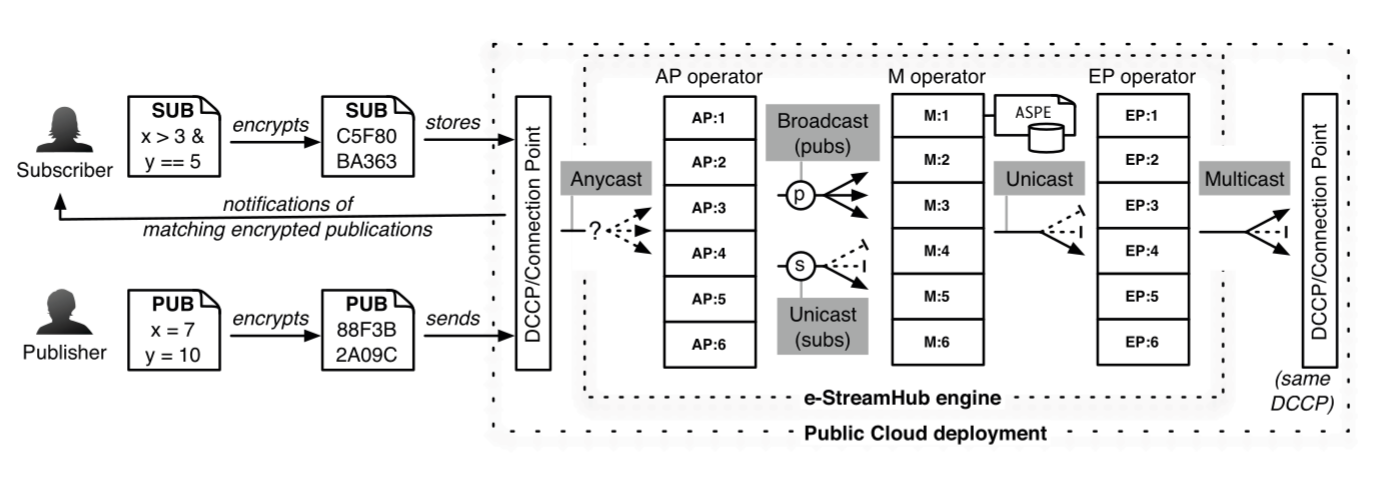
\includegraphics[width=\textwidth]{images/e-strueamhub-arq.png}
    \caption{Ejemplo de un sistema STREAMHUB desplegado en la nube, con 6 instancias de cada operador. Los eventos van de izquierda a derecha. Imagen obtenida de \cite{paper:e-streamhub}.}
    \label{fig:estreamhub-arq}
\end{figure}


La elasticidad de E-StreamHub está implementada mediante la creación de nuevos operadores
en nuevos host cuando estos se necesiten, duplicando los mensajes a procesar en una memoria temporal,
de forma que cuando el nuevo operador esté configurado, pueda comenzar a procesar estos mensajes,
filtrando los obsoletos y minimizando el impacto de esta operación en el sistema.\cite{paper:e-streamhub}

Para poder configurar y manejar los operadores, y las operaciones de creación y eliminación de estos,
E-StreamHub implementa y utiliza un administrador, que monitoriza el estado de los operadores
y lleva a cabo las operaciones de escalado (añadir o eliminar operadores), lo que permite uniformidad
en el sistema y en el manejo de las operaciones de escalado, estableciendo reglas comunes. Al tener
que aplicar una configuración uniforme a todos los operadores, y con el objetivo de poder aplicar esta
configuración y tener control sobre los operadores existentes, E-StreamHub también hace uso
de ZooKeeper\footnote{\href{https://zookeeper.apache.org/}{https://zookeeper.apache.org/}}.

Las reglas a seguir para aplicar las operaciones de escalado se basan en el estado de ciertos recursos
de computación, como el uso de CPU, memoria, etc. Estas reglas, que se aplican para minimizar los
costes a la vez que se maximiza la eficiencia del sistema, se dividen en \textit{locales}, que provocan
que se muevan operadores entre host ya existentes; y \textit{globales}, que hacen que el sistema 
escale, añadiendo o quitando host y moviendo los operadores a otros host con poca carga de trabajo.


%%%%%%%%%%%%%%%%%%%%%%%%%%%%%%%%%%%%%%%%%%%%%%%%%%%%%%%%%%%%%%%%%%%%%%%%%%%%%%%%
%%%%%%%%%%%%%%%%%%%%%%%%%%%%%%%%%%%%%%%%%%%%%%%%%%%%%%%%%%%%%%%%%%%%%%%%%%%%%%%%


\section{Problemas de disponibilidad de cargas de trabajo basadas en contenido} \label{sct:art_sistpubsubcont_problemasdatasetreales}

Uno de los principales problemas actuales en la investigación y desarrollo de sistemas 
publicador/subscriptor es la carencia de cargas de trabajo reales y públicas, que permitan probar los 
sistemas en desarrollo en unas condiciones lo más cercanas a las reales. Estas pruebas son de vital 
importancia para el desarrollo de este tipo de sistemas, ya que ofrecen datos y métricas sobre el
comportamiento final del sistema.

Esta carencia es consecuencia del contenido de los propios datos presentes en las cargas de trabajo,
ya que publicar estas cargas de trabajo puede suponer un problema de seguridad para los usuarios y la
propia empresa que los publica, al contener los intereses (subscripciones) de los
usuarios\cite{paper:lackpublicworkloads}\cite{paper:autoscaling-review}\cite{paper:padres}.


%%%%%%%%%%%%%%%%%%%%%%%%%%%%%%%%%%%%%%%%%%%%%%%%%%%%%%%%%%%%%%%%%%%%%%%%%%%%%%%%
%%%%%%%%%%%%%%%%%%%%%%%%%%%%%%%%%%%%%%%%%%%%%%%%%%%%%%%%%%%%%%%%%%%%%%%%%%%%%%%%


\section{Auto-escalado} \label{sct:art_auto-escaling}

% 0. Contar qué es el auto-escalado
El auto-escalado es la capacidad de un sistema de ajustar (aumentar/disminuir) los recursos computacionales
de os que hace uso de forma automática, en base a la cantidad de trabajo que está recibiendo, y con mínima
o ninguna supervisión humana. Esta característica se ha popularizado en gran medida en los sistemas de
computación en la nube, ya que minimiza los costes en un entorno en el que los recursos son 
\textit{pay-as-you-go}, es decir, solo se paga por los recursos que se usan en cada momento.

Este tipo de sistemas siguen unos requisitos mínimos, especificados en el 
Service Level Agreement o \textit{SLA}, de sus siglas en inglés, el cual es un contrato entre 
el cliente y el propietario de la aplicación. Estos requisitos, por lo general, son las métricas mínimas
del sistema, como por ejemplo, el tiempo de respuesta, el número de mensajes por segundo producidos 
por el sistema (\textit{throughput}\footnote{Para mayor coherencia y brevedad, se usará \textit{throughput} en el resto del documento}).

% 1. Tipos de auto-escalado (especificar el que se va a usar en este trabajo)
El escalado de un sistema puede llevarse a cabo de dos formas diferentes\cite{paper:autoscaling-review}:
\begin{itemize}

    \item[•] \textbf{Escalado horizontal} (\textit{scaling in/out}): añadir o eliminar recursos 
    mediante replicar los ya existentes con el objetivo de balancear el trabajo. Por ejemplo, crear 
    o eliminar una instancia del host para que procese parte del trabajo.

    \item[•] \textbf{Escalado vertical} (\textit{scaling up/down}): añadir o eliminar recursos
    computacionales a un host que ya esté procesando el trabajo recibido. Por ejemplo, aumentar o 
    disminuir la cantidad de CPU dedicada al procesamiento del trabajo recibido.

\end{itemize}

El escalado horizontal es ampliamente usado en los sistemas de computación en la nube, al ofrecer 
mayor flexibilidad a los usuarios en el uso de los recursos 
computacionales\footnote{En este trabajo solo se tratará el escalado horizontal.}. En cambio, el escalado
vertical no se usa en gran medida, ya que, por lo general, los sistemas operativos no permiten cambiar
la cantidad de recursos dedicados a una tarea mientras esta se está llevando a cabo sin reiniciar su 
procesado.

% 2. Mencionar que hay otras clasificaciones de auto-escalables
Adicionalmente, los sistemas auto-escalables se pueden clasificar en reactivos y 
predictivos, es decir, en base a su forma de reaccionar ante una situación que requiera de una 
operación de escalado.

%%%%%%%%%%%%%%%%%%%%%%%%%%%%%%%%%%%%%%%%%%%%%%%%%%%%%%%%%%%%%%%%%%%%%%%%%%%%%%%%

\subsection{Reactivo} \label{ssct:art_auto-escaling_reactive-autoscaling}

Los sistemas auto-escalables que no realizan predicción alguna en la fase de análisis emplean el
\textit{auto-escalado reactivo}, es decir, se limitan a responder al estado actual del sistema,
llevando a cabo las operaciones de escalado requeridas en ese momento, sin tener en cuenta el estado
en el que se podrá encontrar el sistema en el futuro inmediato.

De esta forma, si el sistema se encuentra en una situación en la que la operación de escalado que se 
lleva a cabo no es suficiente para la carga de trabajo que está recibiendo, tendrá que realizar una 
nueva operación de escalado. Este procedimiento puede llevar al sistema, hasta que realice las 
suficientes operaciones de escalado, a proporcionar un servicio por debajo del óptimo y/o esperado.

%%%%%%%%%%%%%%%%%%%%%%%%%%%%%%%%%%%%%%%%%%%%%%%%%%%%%%%%%%%%%%%%%%%%%%%%%%%%%%%%

\subsection{Predictivo} \label{ssct:art_auto-escaling_predictive-autoscaling}

A diferencia del auto-escalado reactivo, el auto-escalado predictivo sí tiene en cuenta el futuro 
inmediato del sistema mediante la aplicación de algoritmos de predicción basados en diferentes métricas,
las cuales pueden basarse, por ejemplo, en el grado de utilización de cierto recurso del sistema en una 
ventana de tiempo previa a la realización de la operación de escalado, en las métricas propias del 
sistema, como tiempos de respuesta, \textit{throughput}, etc.

Este tipo de escalado es capaz de adaptar los recursos disponibles de la forma más óptima del sistema 
a casi cualquier situación en la que aumente la carga de trabajo del sistema, a excepción de los 
incrementos repentinos y sin precedentes, ya que estos son completamente impredecibles.


%%%%%%%%%%%%%%%%%%%%%%%%%%%%%%%%%%%%%%%%%%%%%%%%%%%%%%%%%%%%%%%%%%%%%%%%%%%%%%%%
%%%%%%%%%%%%%%%%%%%%%%%%%%%%%%%%%%%%%%%%%%%%%%%%%%%%%%%%%%%%%%%%%%%%%%%%%%%%%%%%


\section{Cargas de trabajo} \label{sct:art_workloads}

Las cargas de trabajo utilizadas en los sistemas publicador/subscriptor 
representan el número de peticiones de usuarios al sistema, junto con su
tiempo de envío\cite{paper:type_of_workloads}.

Existen 5 tipos de cargas de trabajo en los sistemas de computación en la nube:
\begin{itemize}

    \item \textit{Carga estática}: carga con un número constante de eventos 
    por minuto (ver \autoref{fig:art_workloads-static}).

    \item \textit{Carga creciente}: carga con un rápido incremento en los
    eventos por minuto (ver \autoref{fig:art_workloads-inc}).

    \item \textit{Carga con crecimiento puntual}: carga que presenta un 
    incremento puntual en los eventos por minuto.
    
    \item \textit{Carga periódica}: carga con cambios periódicos en el
    número de eventos por minuto (ver \autoref{fig:art_workloads-periodic}).

    \item \textit{Carga ''On-\&-off''}: carga que presenta periodos en los que
    el número de eventos por minuto es 0 (ver \autoref{fig:art_workloads-periodic}).

    \item \textit{Carga impredecible}: carga que presenta fluctuaciones aleatorias
    en el número de eventos por minuto (ver \autoref{fig:art_workloads-onoff}).

\end{itemize}

En este Trabajo de Fin de Grado, solo se harán uso de las cargas crecientes y 
con crecimiento puntual, al ajustarse a los tipos de pruebas que se desarrollarán, ya 
que estos permitirán, mediante los resultados obtenidos, poder diseñar e implementar
los estudios y/o mejoras necesarias en el auto-escalado del sistema.

\begin{figure}[htpb]
    \centering
    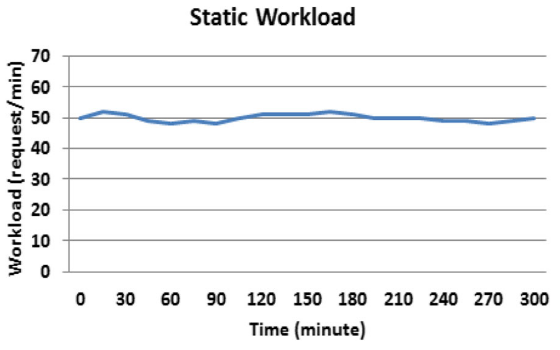
\includegraphics[width=0.5\textwidth]{images/types-of-workload/static-workload.png}
    \caption{\textit{Carga estática.} Imagen obtenida de \cite{paper:type_of_workloads}.}
    \label{fig:art_workloads-static}
\end{figure}

\begin{figure}[htpb]
    \centering
    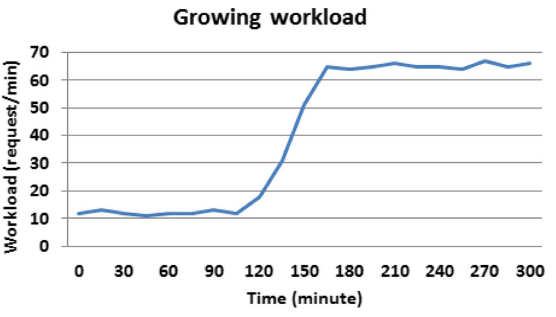
\includegraphics[width=0.5\textwidth]{images/types-of-workload/inc-workload.png}
    \caption{\textit{Carga creciente.} Imagen obtenida de \cite{paper:type_of_workloads}.}
    \label{fig:art_workloads-inc}
\end{figure}

\begin{figure}[htpb]
    \centering
    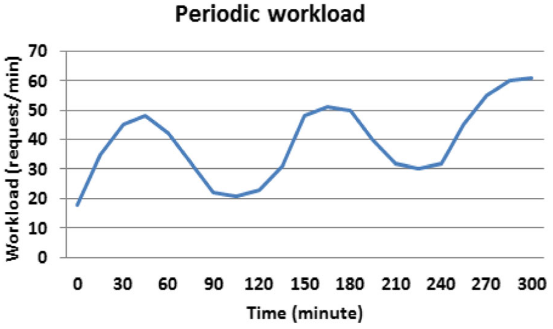
\includegraphics[width=0.5\textwidth]{images/types-of-workload/periodic-workload.png}
    \caption{\textit{Carga periódica.} Imagen obtenida de \cite{paper:type_of_workloads}.}
    \label{fig:art_workloads-periodic}
\end{figure}

\begin{figure}[htpb]
    \centering
    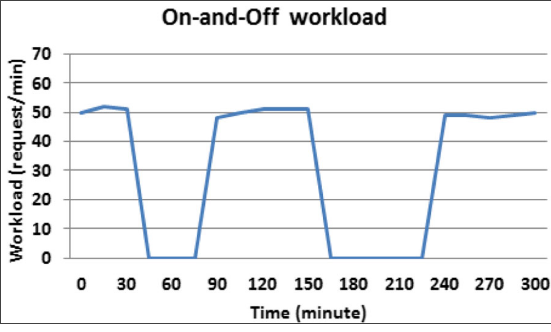
\includegraphics[width=0.5\textwidth]{images/types-of-workload/onoff-workload.png}
    \caption{Carga \textit{''On-\&-off''.} Imagen obtenida de \cite{paper:type_of_workloads}.}
    \label{fig:art_workloads-onoff}
\end{figure}

\begin{figure}[htpb]
    \centering
    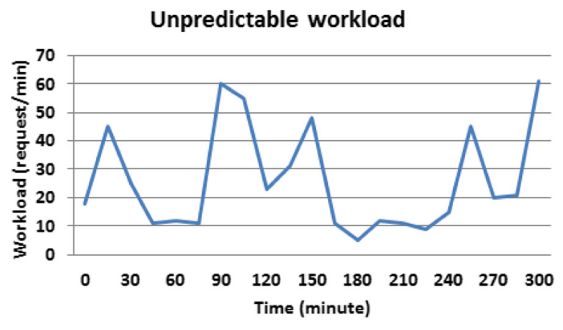
\includegraphics[width=0.5\textwidth]{images/types-of-workload/unpred-workload.png}
    \caption{\textit{Carga inpredecible.} Imagen obtenida de \cite{paper:type_of_workloads}.}
    \label{fig:art_workloads-unpred}
\end{figure}



%%%%%%%%%%%%%%%%%%%%%%%%%%%%%%%%%%%%%%%%%%%%%%%%%%%%%%%%%%%%%%%%%%%%%%%%%%%%%%%%
%%%%%%%%%%%%%%%%%%%%%%%%%%%%%%%%%%%%%%%%%%%%%%%%%%%%%%%%%%%%%%%%%%%%%%%%%%%%%%%%


\section{Estado del Arte} \label{sct:art_stateoftheart}

\subsection{E-SilboPS} \label{ssct:art_stateoftheart_esilbops}

% TFM y Tésis de Victor
% [X] Intro
% [X] Operadores (meter imágen)
% [X] Escalado y algoritmo
% [X] Config (algoritmo ^), comm entre capas (añadir imagen) y Zookeeper

El sistema E-SilboPS, continuación natural del sistema SilboPS y el resultado del 
trabajo de una tesis doctoral\cite{thesis:tesisSVavassori}, es un sistema publicador/subscriptor 
basado en contenido y en contexto, que ha sido diseñado y desarrollado de forma que sea elástico
por defecto.

La arquitectura de este sistema, como se puede comprobar en la \autoref{fig:esilbops-arq} está 
compuesta por cuatro capas de operadores, similar a la encontrada en el sistema 
\textit{StreamHub}\cite{paper:streamhub}, estando cada capa compuesta por una o varias instancias
del correspondiente operador, siendo estos últimos los siguientes:

\textbf{Connection Points (CP)}\\
Estos operadores se encargan de la conexión con los diferentes publicadores y subscriptores y del envío
de las publicaciones correspondientes a los subscriptores interesados en ellas. Los \textit{CP}, que
reciben tanto publicaciones como subscripciones, envían estas a un \textit{Access Point} libre.

\textbf{Access Points (AP)}\\
Los \textit{Access Points}, que reciben publicaciones y subscripciones por igual, se encargan de enviar
la subscripción recibida al \textit{Matcher} seleccionado mediante un selector; mientras que si reciben
una publicación, envían una copia de esta a cada \textit{Matcher}.

\textbf{Matcher (M)}\\
Los \textit{Matchers} almacenan las subscripciones de los usuarios, teniendo cada instancia una pequeña
lista de subscripciones, que serán las que le ha asignado el selector. En cambio, las publicaciones se usan
para comparar los parámetros del contenido deseado por cada subscripción con los de la publicación manejada,
generando una lista de subscriptores interesados en dicha publicación.

\textbf{Exit Points (EP)}\\
Estos operadores, que solo reciben las listas parciales de subscriptores generadas por los \textit{Matchers}
y la publicación correspondiente, componen una lista completa de subscriptores interesados en dicha 
publicación.

\begin{figure}[htpb]
    \centering
    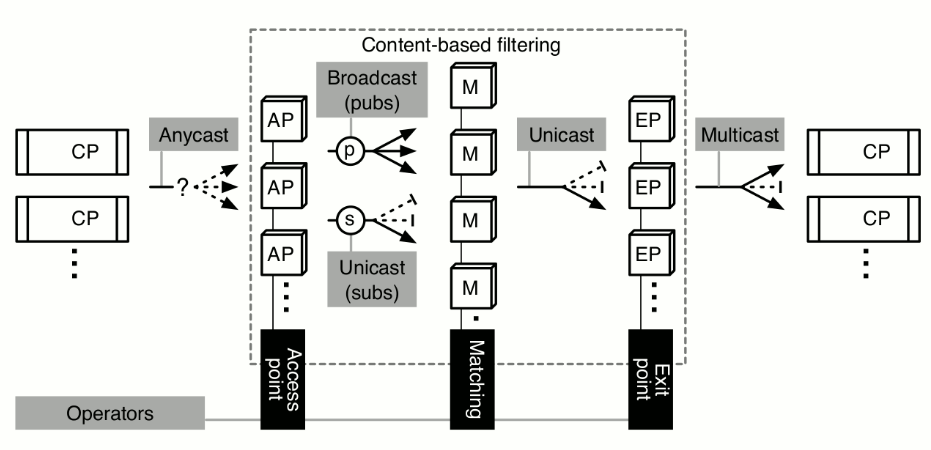
\includegraphics[width=\textwidth]{images/streamhub-arq.png}
    \caption{Arquitectura y funcionamiento de los sistemas \textit{E-SilboPS} y \textit{StreamHub}. Imagen obtenida de \cite{paper:e-streamhub}.}
    \label{fig:esilbops-arq}
\end{figure}

La elasticidad de \textit{E-SilboPS} se basa en la capacidad de cada capa de operadores de añadir o quitar
instancias (operaciones de escalado) de los operadores correspondientes de forma dinámica, ajustando la
capacidad del sistema a los requisitos de este en cada momento, optimizando el uso de los recursos 
computacionales al máximo.

Esta escalabilidad dinámica sin interrumpir el sistema se lleva a cabo gracias al algoritmo de escalado, basado
en el algoritmo de Chandy-Lamport\cite{paper:chandy-lamport}, que permite al sistema seguir operando de
forma normal incluso cuando se está llevando a cabo una operación de escalado.

De forma adicional, y para poder mantener la coordinación y comunicación entre las diferentes capas de 
operadores del sistema, como se observa en la \autoref{fig:esilbops-opcomm} y la consistencia y estabilidad 
del mismo, se requiere del uso de un administrador, que imponga la configuración establecida para cada y su 
coordinación con las demás. El sistema elegido para llevar a cabo esta tarea es
Zookeeper\footnote{\href{https://zookeeper.apache.org/}{https://zookeeper.apache.org/}}.

\begin{figure}[htpb]
    \centering
    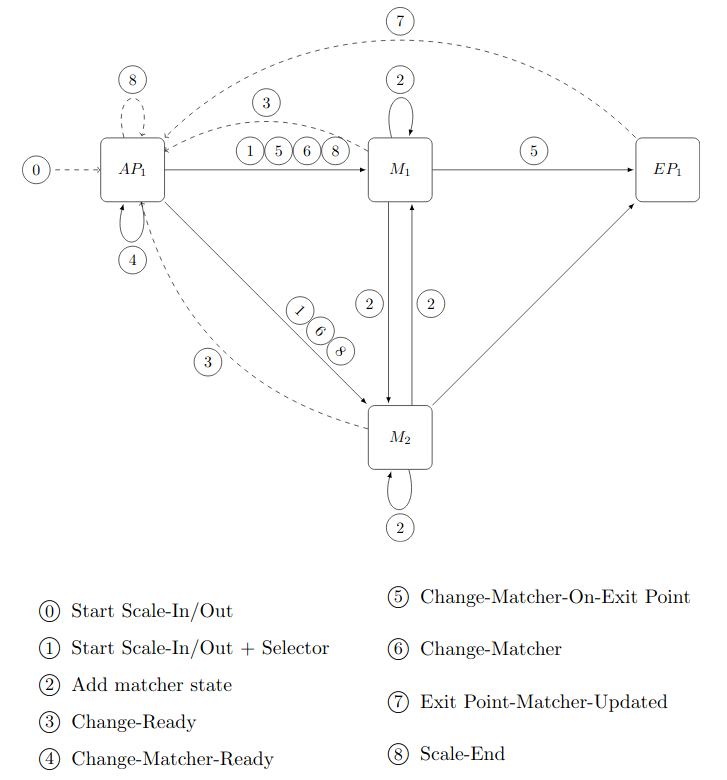
\includegraphics[width=\textwidth]{images/esilbops-opcomm.png}
    \caption{Comunicación y coordinación de las capas de operadores en una operación de escalado de la capa de \textit{Matchers} (M2 es la nueva instancia de \textit{Matcher}). Las lineas continuas representan la comunicación de subscripciones y publicaciones entre capas de operadores, mientras que las discontinuas son mensajes de coordinación para sincronizar las capas y los operadores. Imagen obtenida de \cite{thesis:tesisVictor}.}
    \label{fig:esilbops-opcomm}
\end{figure}

La configuración del sistema y el número de operadores en cada capa se expresa mediante el 
formato \textit{X-Y-Z}, siendo este el número de instancias de los operadores 
\textit{CP}/\textit{AP}, \textit{M} y \textit{EP}, respectivamente.
A lo largo de este documento se usará este formato para expresar la configuración del sistema.


%%%%%%%%%%%%%%%%%%%%%%%%%%%%%%%%%%%%%%%%%%%%%%%%%%%%%%%%%%%%%%%%%%%%%%%%%%%%%%%%
%%%%%%%%%%%%%%%%%%%%%%%%%%%%%%%%%%%%%%%%%%%%%%%%%%%%%%%%%%%%%%%%%%%%%%%%%%%%%%%%


\section{Herramientas utilizadas}

\subsection*{Java}

Java\footnote{\href{https://www.java.com/es/}{https://www.java.com/es/}} es un 
lenguaje de programación orientado a objetos y que sigue un paradigma imperativo.
Ver logo en \autoref{fig:java-logo}.

Tanto E-SilboPS, como los proyectos anteriores se han implementado en Java, por
lo que este trabajo utiliza este lenguaje para desarrollar las pruebas necesarias
para medir el rendimiento del sistema.

\begin{figure}[htpb]
    \centering
    
\includegraphics[width=0.3\linewidth]{images/logos/java-logo.png} 
    \caption{Logo de Java.}
    \label{fig:java-logo}
\end{figure}


\subsection*{R}

R\footnote{\href{https://www.r-project.org/}{https://www.r-project.org/}} es un
lenguaje de programación orientado al análisis estadístico. Ver logo 
en \autoref{fig:r-logo}.

Se ha utilizado R para la realización de las cargas de trabajo, y la generación
de las gráficas incluidas en este TFG, así como la implementación de los modelos
predictivos, debido a la versatilidad y cantidad de herramientas que proporciona
para llevar a cabo estas tareas.

\begin{figure}[htpb]
    \centering
    
\includegraphics[width=0.2\linewidth]{images/logos/R-Logo.png} 
    \caption{Logo de R.}
    \label{fig:r-logo}
\end{figure}


\subsection*{Git}

Git\footnote{\href{https://git-scm.com/}{https://git-scm.com/}} es una herramienta
abierta y de código libre para el control de versiones diseñada para facilitar el
manejo de proyectos, principalmente de código. Ver logo en \autoref{fig:git-logo}.

Para mantener coherencia en el desarrollo y tener un control de versiones del
código, se ha utilizado Git, además de 
GitHub\footnote{\href{https://github.com/}{https://github.com/}} y
GitLab\footnote{\href{https://github.com/}{https://github.com/}}, herramientas web
necesarias para facilitar el manejo y gestión de las diferentes ramas y de los
cambios realizados.


\begin{figure}[htpb]
    \centering
    
\includegraphics[width=0.3\linewidth]{images/logos/git-logo.png} 
    \caption{Logo de Git.}
    \label{fig:git-logo}
\end{figure}


\subsection*{Apache Maven}

Maven\footnote{\href{https://maven.apache.org/index.html}{https://maven.apache.org/index.html}}
es una herramienta para el gestión y creación de proyectos Java, ofreciendo un modelo
de configuración muy accesible y sencillo de manejar para el desarrollador. 
Ver logo en \autoref{fig:maven-logo}.

Se ha utilizado Apache Maven debido a su uso previo en este proyecto, así como la
facilidad que proporciona a los desarrolladores para gestionar proyectos Java.

\begin{figure}[htpb]
    \centering
    
\includegraphics[width=0.3\linewidth]{images/logos/maven-logo.png} 
    \caption{Logo de Apache Maven.}
    \label{fig:maven-logo}
\end{figure}


\subsection*{JUnit 5}

JUnit 5\footnote{\href{https://junit.org/junit5/}{https://junit.org/junit5/}} es un
framework para el desarrollo de pruebas para aplicaciones Java que ha sido ampliamente
usado. Ver logo en \autoref{fig:junit5-logo}.

Para implementar las pruebas del generador de cargas de trabajo reales, así como
las pruebas propias el sistema E-SilboPS, se han usado pruebas de JUnit 5.
Este framework permite validar de forma muy completa el funcionamiento de una
aplicación Java, pudiendo probar y confirmar que el comportamiento y las funciones
de un sistema son las esperadas.

\begin{figure}[htpb]
    \centering
    
\includegraphics[width=0.3\linewidth]{images/logos/junit5-logo.png} 
    \caption{Logo de JUnit 5.}
    \label{fig:junit5-logo}
\end{figure}


%%%%%%%%%%%%%%%%%%%%%%%%%%%%%%%%%%%%%%%%%%%%%%%%%%%%%%%%%%%%%%%%%%%%%%%%%%%%%%%%
%%%%%%%%%%%%%%%%%%%%%%%%%%%%%%%%%%%%%%%%%%%%%%%%%%%%%%%%%%%%%%%%%%%%%%%%%%%%%%%%
\chapter{Desarrollo de un generador de cargas de trabajo para sistemas publish/subscribe 
basados en contenido} \label{chp:desarrollo}

En esta sección se expone el trabajo realizado durante el desarrollo de este
generador, así como su contexto y motivación, y los resultados obtenidos.

%%%%%%%%%%%%%%%%%%%%%%%%%%%%%%%%%%%%%%%%%%%%%%%%%%%%%%%%%%%%%%%%%%%%%%%%%%%%%%%%
%%%%%%%%%%%%%%%%%%%%%%%%%%%%%%%%%%%%%%%%%%%%%%%%%%%%%%%%%%%%%%%%%%%%%%%%%%%%%%%%

\section{Motivación} \label{sct:desarrollo_motivacion}

% Necesidad de probar E-SilboPS con dataset real
La necesidad de este generador se origina en la dificultad de probar el sistema \textit{E-SilboPS}
con cargas de trabajo con datos reales (\ref{sct:art_sistpubsubcont_problemasdatasetreales}), 
habiendo sido probado solo con cargas de trabajo sintéticas (artificiales),
es decir, generadas por un programa en base a ciertos parámetros estadísticos (número de 
subscripciones totales, número de subscripciones por segundo, número de notificaciones, 
número de notificaciones por segundo, etc).

% Escasez de dataset reales (ya contado un millón de veces)
El principal problema con este tipo de pruebas es que no reflejan el comportamiento que tendrá
el sistema en un entorno real, incluso cuando las cargas generadas intentan reflejar dicho entorno.
Para solventar esto, se necesita una carga de trabajo real compatible con este sistema.

Para llevar a cabo estas pruebas con la carga de trabajo real, se necesita generar, a partir
de esta, una carga compatible con \textit{E-SilboPS}, transformando cada evento al formato aceptado
por este sistema, preservando el orden y contexto original.

%%%%%%%%%%%%%%%%%%%%%%%%%%%%%%%%%%%%%%%%%%%%%%%%%%%%%%%%%%%%%%%%%%%%%%%%%%%%%%%%
%%%%%%%%%%%%%%%%%%%%%%%%%%%%%%%%%%%%%%%%%%%%%%%%%%%%%%%%%%%%%%%%%%%%%%%%%%%%%%%%

\section{Carga de trabajo} \label{sct:desarrollo_carga}

Esta carga de trabajo se ha extraído del repositorio de \textit{datasets} del 
\textit{Middleware Systems Research Group}\footnote{\href{http://msrg.org/}{http://msrg.org/}}
de la Universidad de Toronto, y pertenece al proyecto
\textit{Mammoth}\footnote{\href{http://msrg.org/datasets/mammoth}{http://msrg.org/datasets/mammoth}},
que se ha creado por medio de obtener la información de los eventos de un juego 
\textit{MMO}\footnote{\textit{Massive Multiplayer Online Game} - Videojuego online con multitud de 
jugadores a través de Internet} que funciona mediante un sistema \textit{publish-subscribe} basado
en contenido.

Además de haberse generado a partir de un sistema similar al que se ha usado en este proyecto, es lo 
suficientemente amplia para llevar a cabo las pruebas necesarias en nuestro sistema, y presenta un
elevado número de subscripciones y de-subscripciones, cualidad necesaria para comprobar las 
fluctuaciones causadas por los incrementos y decrementos de la cantidad de trabajo recibida.

%%%%%%%%%%%%%%%%%%%%%%%%%%%%%%%%%%%%%%%%%%%%%%%%%%%%%%%%%%%%%%%%%%%%%%%%%%%%%%%%

\subsection{Análisis estático} \label{ssct:desarrollo_carga_analisis}

% Análisis del dataset
% - Análisis estático
%  + Objetivo del análisis
%  + Comparar formatos (incluir figuras con ambos formatos)

Previo uso de la carga, se ha llevado a cabo un análisis estático, con el objetivo de comprobar su
compatibilidad con el formato de los eventos de \textit{E-SilboPS} y la integridad de los propios 
datos, y, además, poder conocer de antemano datos estadísticos relevantes para el futuro desarrollo
y especificación de pruebas que la usen.

Mediante este análisis, se ha obtenido la siguiente información básica sobre la carga de trabajo:
\begin{itemize}
    \item[•] La marca de tiempo (\textit{timestamp})\footnote{En este trabajo, el término
    \textit{timestamps} y \textit{marca de tiempo} se usarán de forma intercambiable}, está
    compuesta por \texttt{13} dígitos, a diferencia de la de \textit{Linux}, de \texttt{10} dígitos.
    \item[•] Contiene mensajes de error (\texttt{[ERROR] ...}), que han de ser eliminados.
    \item[•] Tiene mensajes generados de manera simultánea, ya que el \textit{timestamp} de algunos
    mensajes es igual.
\end{itemize}

De forma adicional, se ha generado la siguiente información estadística, útil para el desarrollo 
futuro de este proyecto:
\begin{itemize}
    \item[•] Número de subscripciones: \texttt{113.904}
    \item[•] Número de de-subscripciones: \texttt{112.682}
    \item[•] Número de publicaciones: \texttt{6.207.207}
\end{itemize}

Con el objetivo de comprobar la correctitud de los eventos de la carga de trabajo, se ha verificado
que la carga no contiene subscripciones y de-subscripciones duplicadas, o de-subscripciones antes que 
la subscripción correspondiente.

%%%%%%%%%%%%%%%%%%%%%%%%%%%%%%%%%%%%%%%%%%%%%%%%%%%%%%%%%%%%%%%%%%%%%%%%%%%%%%%%

\subsection{Formato y operadores} \label{ssct:desarrollo_carga_formato}

Para concluir el análisis estático, se han comparado los formatos de cada tipo 
de eventos que, de acuerdo a la documentación de Mammoth\cite{paper:mammoth_paper} 
y E-SilboPS\cite{thesis:tesisVictor}, ambos sistemas cuentan con los siguientes
operadores para los pares clave-valor de sus eventos.

\begin{table}[htpb]
    \centering
    \begin{tabular}{|c|c|c|}
        \hline
        \textbf{E-SilboPS} & \textbf{Mammoth} & \textbf{Descripción} \\
        \hline
        \texttt{\{''exists'': ...\}}   & -  & El atributo existe \\
        \texttt{\{''='': ...\}}        & \texttt{eq} & Igual \\
        \texttt{\{''!='': ...\}}       & -  & No igual \\
        \texttt{\{''>'': ...\}}        & -  & Mayor que \\
        \texttt{\{''>='': ...\}}       & -  & Mayor o igual que \\
        \texttt{\{''<'': ...\}}        & -  & Menor que \\
        \texttt{\{''<='': ...\}}       & -  & Menor o igual que \\
        \texttt{\{''\^'': ...\}}       & -  & Comienza con el prefijo \\
        \texttt{\{''\$'': ...\}}       & -  & Termina con el sufijo \\
        \texttt{\{''contains'': ...\}} & -  & Contiene \\
        \hline
    \end{tabular}
    \caption{Tabal comparativa de operadores de \textit{E-SilboPS} y \textit{Mammoth}}
    \label{tab:comparadores}
\end{table}

Como se observa en el \autoref{tab:comparadores}, estos sistemas solo comparten el operador
de igualdad (\texttt{eq}), por lo que la carga de trabajo generada solo contendrá este operador 
para todas las pares clave-valor de cada uno de los eventos presentes en la misma.

El formato de los eventos en ambos sistemas son también diferentes entre sí para los tres tipos 
de eventos que manejan, siendo el formato de las subscripciones, como se ve en los
\autoref{lst:esilbops_sub} y \autoref{lst:mammoth_sub}, compatible, pues los 
\textit{''constraints''} son las claves y valores que se comprueban contra las publicaciones,
que en \textit{Mammoth} son los valores entre corchetes, mientras que el valor entre llaves es
el \textit{timestamp} de la subscripción, la cual solo se usará para mantener el orden de los
eventos en el fichero.\\

\begin{lstlisting}[caption={Ejemplo de subscripción de E-SilboPS.},label={lst:esilbops_sub}, style=consola,captionpos=b]
{
	"id" : "",
	"contextFunction": {},
	"constraints": {
		"symbol:str": [{"=": "GOOG"}],
		"value:double": [{">": 100.25}, {"<=": 500.0}],
		"volume:long": [{">=": 1000}],
		"timestamp:long": [{"exists": ""}]
	}
}
\end{lstlisting}

\begin{lstlisting}[caption={Ejemplo de subscripción de Mammoth.}, label={lst:mammoth_sub}, style=consola,captionpos=b]
{1307423528250} s [class,eq,broadcast] (rmi://10.0.1.2:1099/Broker2-M4894)
\end{lstlisting}

A diferencia que en \textit{Mammoth}, como se ve en \autoref{lst:esilbops_unsub} y 
\autoref{lst:mammoth_unsub}, el formato de las de-subscripciones en \textit{E-SilboPS} 
es igual al de las subscripciones. A pesar de esto, la compatibilidad se mantiene.

\begin{lstlisting}[caption={Ejemplo de de-subscripcion de E-SilboPS.},label={lst:esilbops_unsub},style=consola,captionpos=b]
{
	"id" : "",
	"contextFunction": {},
	"constraints": {
		"symbol:str": [{"=": "GOOG"}],
		"value:double": [{">": 100.25}, {"<=": 500.0}],
		"volume:long": [{">=": 1000}],
		"timestamp:long": [{"exists": ""}]
	}
}
\end{lstlisting}

\begin{lstlisting}[caption={Ejemplo de de-subscripción de Mammoth.},label={lst:mammoth_unsub},style=consola,captionpos=b]
{1307425244397} us rmi://10.0.1.4:1099/Broker4-M81393
\end{lstlisting}

En las publicaciones, el formato de ambos sistemas son muy similares y compatibles, como se puede ver
en \autoref{lst:esilbops_pub} y \autoref{lst:mammoth_pub}.

\begin{lstlisting}[caption={Ejemplo de publicación de E-SilboPS.},label={lst:esilbops_pub},style=consola,captionpos=b]
{
	 "symbol:str" : "GOOG",
	 "value:double" : 333.2,
	 "volume:long" : 345
}
\end{lstlisting}

\begin{lstlisting}[caption={Ejemplo de publicación de Mammoth.},label={lst:mammoth_pub},style=consola,captionpos=b]
{1307422272885} p [class,ProxyID_-3884500000][x,0.0][y,0.0]
\end{lstlisting}



%%%%%%%%%%%%%%%%%%%%%%%%%%%%%%%%%%%%%%%%%%%%%%%%%%%%%%%%%%%%%%%%%%%%%%%%%%%%%%%%
%%%%%%%%%%%%%%%%%%%%%%%%%%%%%%%%%%%%%%%%%%%%%%%%%%%%%%%%%%%%%%%%%%%%%%%%%%%%%%%%

\section{Diseño} \label{sct:desarrollo_diseno}

El programa deberá leer cada línea del fichero de entrada, es decir, la carga de trabajo
proveniente de \textit{Mammoth}, interpretar cada evento y generar el mismo evento en el formato 
compatible con \textit{E-SilboPS}, manteniendo los datos y el orden de los mismos. El fichero generado 
debe ser en formato \textit{JSON}\footnote{JavaScript Object Notation}, ya que es ese el
formato de los eventos de \textit{E-SilboPS}.

En este sistema, al tener las subscripciones y las de-subscripciones el mismo formato, el generador
tiene que ser capaz de guardar todas las subscripciones que haya generado, y generar las 
de-subscripciones de las mismas cuando así lo lea del fichero de entrada.

De igual forma, ha de ser capaz de detectar errores en los eventos leídos,
comprobando la correcta estructura de cada regla, sus valores, y sus operadores.

% No se me ocurre que más poner, no es tan complejo el generador

%%%%%%%%%%%%%%%%%%%%%%%%%%%%%%%%%%%%%%%%%%%%%%%%%%%%%%%%%%%%%%%%%%%%%%%%%%%%%%%%
%%%%%%%%%%%%%%%%%%%%%%%%%%%%%%%%%%%%%%%%%%%%%%%%%%%%%%%%%%%%%%%%%%%%%%%%%%%%%%%%

\section{Implementación} \label{sct:desarrollo_implementacion}

El generador se ha implementado en el lenguaje de programación
\textit{Java}\footnote{\href{https://www.java.com/en/}{https://www.java.com/en/}}, utilizando
las herramientas, \textit{Maven}\footnote{\href{https://maven.apache.org/}{https://maven.apache.org/}} 
para gestionar el proyecto y sus dependencias, y 
\textit{JUnit5}\footnote{\href{https://junit.org/junit5/}{https://junit.org/junit5/}} para realizar
pruebas y comprobar el correcto funcionamiento del programa.

A partir del diseño propuesto, se ha creado y seguido la estructura de clases que se ve en la 
\autoref{fig:parser_uml}, estableciendo una estructura de funciones transparente al usuario.

\begin{figure}[htpb]
    \centering
    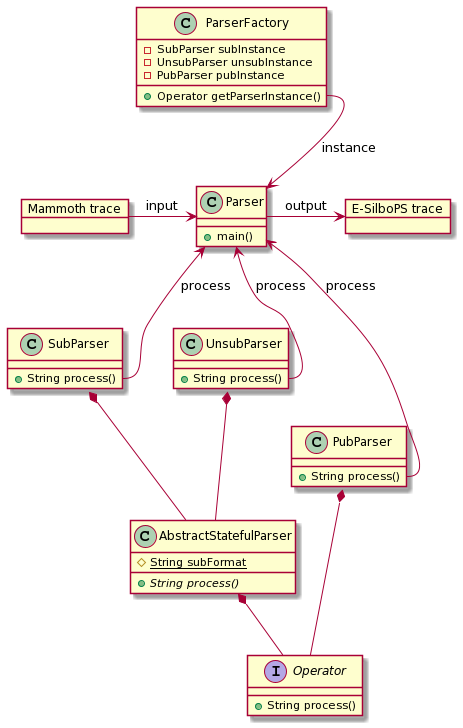
\includegraphics[width=0.75\textwidth]{images/plantuml/ParserPlantUML.png}
    \caption{Diagrama de clases del generador de cargas de trabajo reales.}
    \label{fig:parser_uml}
\end{figure}

Las clases y sus funciones mostradas en la figura \autoref{fig:parser_uml} se han simplificado para 
facilitar su lectura y comprensión general, ya que no se han incluido estructuras de datos internas
y los tipos de las mismas por ser únicamente de uso interno.

Para facilitar la lectura del fichero \textit{JSON} de salida, este se ha implementado como una lista,
o \textit{array}, de objetos \textit{JSON}, de forma que la prueba que lea dicho fichero solo tenga
que leer cada uno de estos elementos en la lista para poder usarlos, sin necesidad de realizar más
operaciones, las cuales serían necesarias si el fichero de salida no siguiese este formato.

Una vez implementado el generador, y habiendo generado el fichero \textit{JSON} que representa la carga
de trabajo real en el formato de \textit{E-SilboPS}, se puede comenzar el desarrollo de las pruebas
necesarias en este sistema usando esta carga.

%%%%%%%%%%%%%%%%%%%%%%%%%%%%%%%%%%%%%%%%%%%%%%%%%%%%%%%%%%%%%%%%%%%%%%%%%%%%%%%%
%%%%%%%%%%%%%%%%%%%%%%%%%%%%%%%%%%%%%%%%%%%%%%%%%%%%%%%%%%%%%%%%%%%%%%%%%%%%%%%%

\section{Pruebas en E-SilboPS} \label{sct:desarrollo_pruebas-esilbops}

Una vez generada la carga de trabajo deseada, se han creado las siguientes pruebas que la usan, con 
el objetivo de comprobar el comportamiento del sistema por medio de sus principales métricas de 
rendimiento, de forma que se obtenga una visión general del sistema a lo largo del tiempo.

Como no todas las publicaciones generan subscripciones, es necesario introducir dos nuevos eventos
(una subscripción al inicio (ver \autoref{lst:mammoth_subflag}), y una publicación al final 
(ver \autoref{lst:mammoth_pubflag})), a la carga, que solo se enviará una única vez, marcando el
final de la prueba correspondiente.

\begin{minipage}[t]{.5\textwidth}
\begin{lstlisting}[caption={Subscripción en E-SilboPS para identificar el final de la carga.}, label={lst:mammoth_subflag}, style=consola,captionpos=b]
{
	"id" : "MAMMOTH_FLAG"
	"contextFunction" : {},
	"constraints" : {
		"class:str" : [{"=" : "END"}]
	}
}
\end{lstlisting}
\end{minipage}
\hfill
\begin{minipage}[t]{.45\textwidth}
\begin{lstlisting}[caption={Publicación en E-SilboPS que marca el final de la carga.}, label={lst:mammoth_pubflag}, style=consola,captionpos=b]
{
    "id:long" : 0
    "class:str" : "END"
}
\end{lstlisting}
\end{minipage}

Una vez diseñados e implementados estos conceptos, se han implementado las 
siguientes pruebas, usando una topología 1-1-1 (1 EP, 1 M, 1 EP) en E-SilboPS,
siendo el emisor y el receptor diferentes hilos (\textit{threads}) de un mismo
computador.

%%%%%%%%%%%%%%%%%%%%%%%%%%%%%%%%%%%%%%%%%%%%%%%%%%%%%%%%%%%%%%%%%%%%%%%%%%%%%%%%

\subsection{Velocidad fija de envío} \label{ssct:desarrollo_pruebas-esilbops_test-fixed}

Para esta primera prueba, se ha procedido al envío de toda la carga de trabajo,
subscripciones, de-subscripciones y publicaciones, a diferentes velocidades
de envío (ver lista a continuación) mediante repetir esta prueba con cada una
de ellas.

\begin{itemize}
    \item 50.000 mensajes por segundo.
    \item 100.000 mensajes por segundo.
    \item 200.000 mensajes por segundo.
    \item 500.000 mensajes por segundo.
    \item 1.000.000 mensajes por segundo.
    \item 6.433.794 mensajes por segundo (máxima velocidad posible).
\end{itemize}

Parámetros adicionales de estas pruebas:
\begin{itemize}
    \item Número de publicaciones: 6.207.207
    \item Número de subscripciones: 113.904
    \item Número de de-subscripciones: 112.682
    \item Número de notificaciones: 4.515.781 (72\% de las publicaciones machean)
    \item Cada publicación machea como máximo, con una única subscripción.\footnote{Esto
    se tendrá en cuenta para el desarrollo de futuras pruebas.}
\end{itemize}

Para poder obtener los datos más precisos, se ha decidido medir el tiempo de respuesta una vez cada 
50.000 notificaciones recibidas\footnote{Esta característica se ha mantenido en todas las pruebas 
realizadas}, ya que medir más frecuentemente provoca una distorsión en las mediciones y por
ende, en su interpretación.

%%%%%%%%%%%%%%%%%%%%%%%%%%%%%%%%%%%%%%%%%%%%%%%%%%%%%%%%%%%%%%%%%%%%%%%%%%%%%%%%

\subsection{Secuencia logarítmica de subscripciones} \label{ssct:desarrollo_pruebas-esilbops_test-log}

En esta prueba, se separan las subscripciones y las publicaciones, enviando las subscripciones
siguiendo una secuencia logarítmica (comenzando en 100 subscripciones), hasta haber enviado todas
las subscripciones (113.904). Este proceso se muestra en la \autoref{fig:testlog-uml}). 
Tras enviar las nuevas subscripciones, se envían todas las publicaciones de la carga, midiendo el
throughput total del sistema.

Parámetros de la prueba:
\begin{itemize}
    \item Número de publicaciones: 6.207.207
    \item Subscripciones en secuencia logarítmica, de 100 a 113.904 (todas las subscripciones)
    \item La prueba se repetirá 10 veces por cada punto en la gráfica, siendo el valor final
    de este la media del throughput total de cada repetición.
    \item Velocidad de envío (input rate): 100.000 mensajes por segundo.
\end{itemize}

\begin{figure}[htpb]
    \centering
    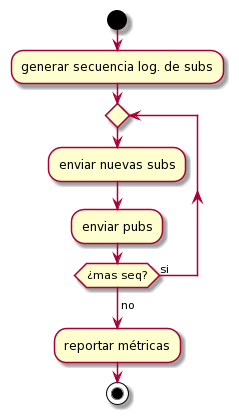
\includegraphics[width=0.35\textwidth]{images/plantuml/testlog-plantuml.png}
    \caption{Diagrama de ejecución de prueba con subscripciones en secuencia logarítmica.}
    \label{fig:testlog-uml}
\end{figure}

%%%%%%%%%%%%%%%%%%%%%%%%%%%%%%%%%%%%%%%%%%%%%%%%%%%%%%%%%%%%%%%%%%%%%%%%%%%%%%%%

\subsection{Carga de subscripciones creciente} \label{subsct:desarrollo_pruebas-esilbops_test-inc}

Para llevar a cabo esta prueba, primero se ha generado una traza de números 
(ver \autoref{fig:subs_workload-growing}) con un incremento constante hasta 
llegar a un número deseado, y manteniendo dicho número hasta el final de la misma.

Esta traza de números (\autoref{fig:subs_workload-growing}) representa el 
número de subscripciones presentes en cada momento (ver 
\autoref{sct:art_workloads}), con cierto ruido/fluctuaciones, simulando un
entorno real con nuevas subscripciones y de-subscripciones cada segundo.

Parámetros de la prueba:
\begin{itemize}
    \item Subscripciones base: 10.000
    \item Subscripciones finales: 20.000
    \item Ruido: $\pm$ 2000 subscripciones
    \item Tiempo de la prueba: 600 segundos
    \item Velocidad de envío (input rate): 50.000 mensajes por segundo
\end{itemize}

\begin{figure}[htpb]
    \centering
    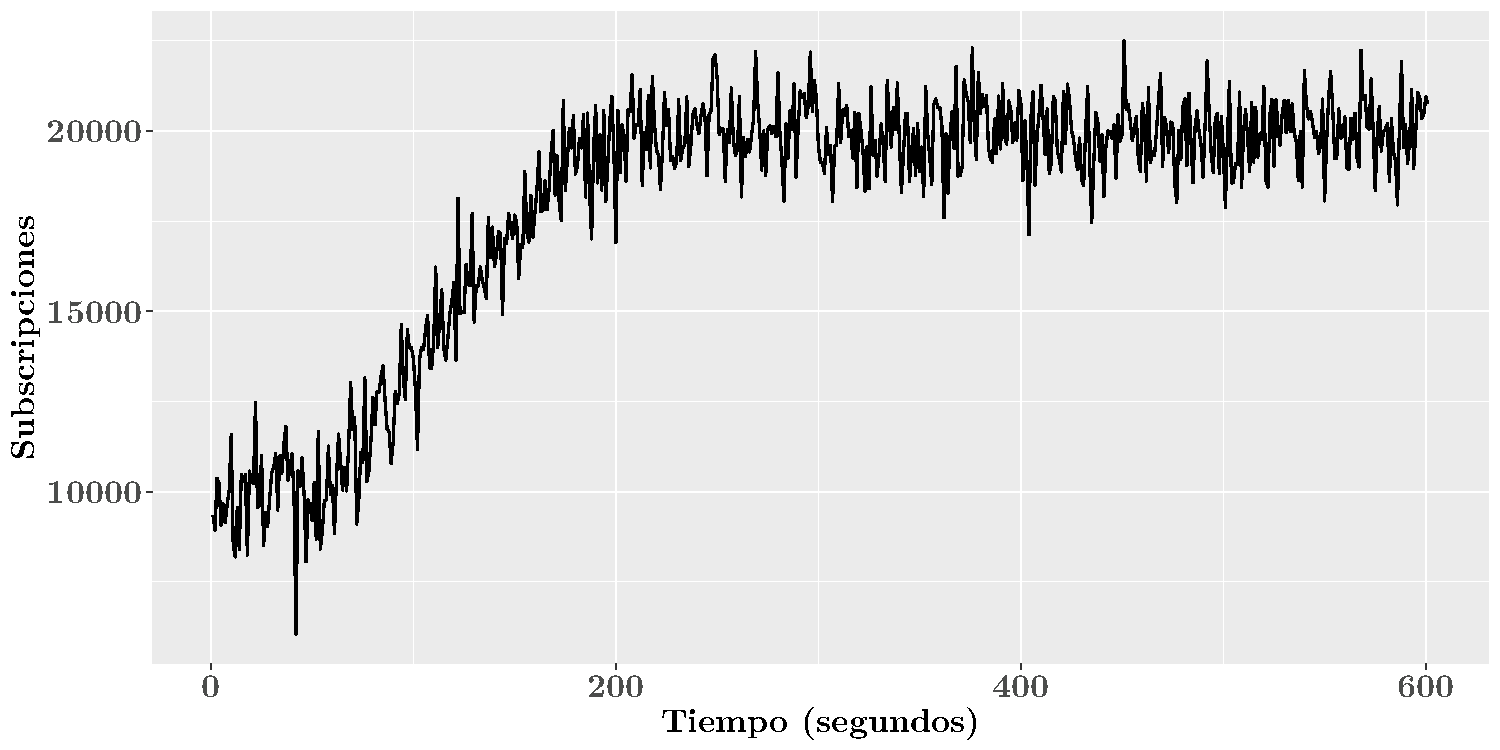
\includegraphics[width=\textwidth]{images/workload-types/subs_workload-growing.pdf}
    \caption{Ejemplo de carga de trabajo creciente (con ruido añadido).}
    \label{fig:subs_workload-growing}
\end{figure}

% Introducir el resto de trazas de este tipo (nonoise, unique-pub, unique-pubsub)

Esta traza es leída por la prueba, y, en base al número presente de subscripciones en el sistema,
genera nuevas subscripciones o de-subscripciones, de forma que, cada segundo, el sistema contenga
el número de subscripciones especificadas en esta, siguiendo el flujo de ejecución que se muestra 
en la \autoref{fig:testinc-uml}).

El envío de publicaciones se realiza a un ratio fijo por segundo (input rate), y de forma paralela al envío de 
subscripciones/de-subscripciones, interpretando las publicaciones como una lista circular hasta
que se haya recorrido toda la traza de subscripciones. Una vez esto sucede, se envían las restantes 
publicaciones y finaliza la prueba.

\begin{figure}[htpb]
    \centering
    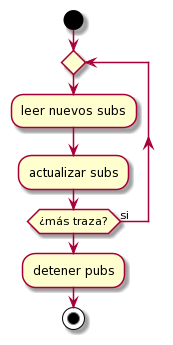
\includegraphics[width=0.35\textwidth]{images/plantuml/testinc-plantuml.png}
    \caption{Diagrama de ejecución de la prueba con carga de trabajo incremental.}
    \label{fig:testinc-uml}
\end{figure}

\subsection{Carga de subscripciones estática} \label{subsct:desarrollo_pruebas-esilbops_test-static}

Estas pruebas se han basado en la confección de una carga de trabajo basada en
la real (ver \autoref{sct:art_workloads}, \textit{Carga estática}), 
en la cual la cantidad de subscriptores no cambia durante toda la 
ejecución de dicha prueba, es decir, se envía un número determinado de subscripciones
al inicio de la prueba, y se mantienen esas subscripciones hasta acabar esta.

Junto con estas carga, se debe de especificar la velocidad a la que el sistema 
envía las publicaciones (input rate), para simular un entorno en el que el 
sistema recibe muchos eventos por segundo, que han de ser procesados y enviados,
con el objetivo de ver el punto en el que el sistema satura parcialmente.

En estas pruebas, el ratio al que se envían las publicaciones será mayor que en 
las siguientes pruebas, ya que el sistema no está procesando nuevas subscripciones
o desubscripciones, solo publicaciones entrantes.

Parámetros de las pruebas:
\begin{itemize}
    \item Dos pruebas, una con 50.000 subscripciones, otra con 100.000 subscripciones
    \item Tiempo de la prueba: 600 segundos
    \item Velocidad de envío (input rate): 200.000 mensajes por segundo
\end{itemize}

\subsection{Carga de subscripciones con crecimiento puntual} \label{subsct:desarrollo_pruebas-esilbops_test-spike}

Siguiendo con estas pruebas, se han desarrollado unas cargas de trabajo que presentan
un incremento de las subscripciones puntual, es decir, las subscripciones comienzan
constantes, y tras un periodo de tiempo, incrementan hasta cierto valor. Una vez se
llega a ese valor, todas esas nueva subscripciones se eliminan mediante el envío de
las desubscripciones correspondientes.

Subscripciones de las pruebas:
\begin{itemize}
    \item Crecimiento de 20.000 a 100.000 subscripciones (\autoref{fig:subsworkload_20k-100k})
    \item Crecimiento de 25.000 a 113.904 subscripciones (\autoref{fig:subsworkload_25k-113k})
    \item Crecimiento rápido de 25.000 a 113.904 subscripciones (\autoref{fig:subsworkload_fast_spike_25k-113k-100k})
\end{itemize}

Parámetros de las pruebas:
\begin{itemize}
    \item Publicaciones: buffer circular de 6.207.207 publicaciones
    \item Velocidad de envío (input rate): 125.000 mensajes por segundo
\end{itemize}

\begin{figure}[htpb]
    \centering
    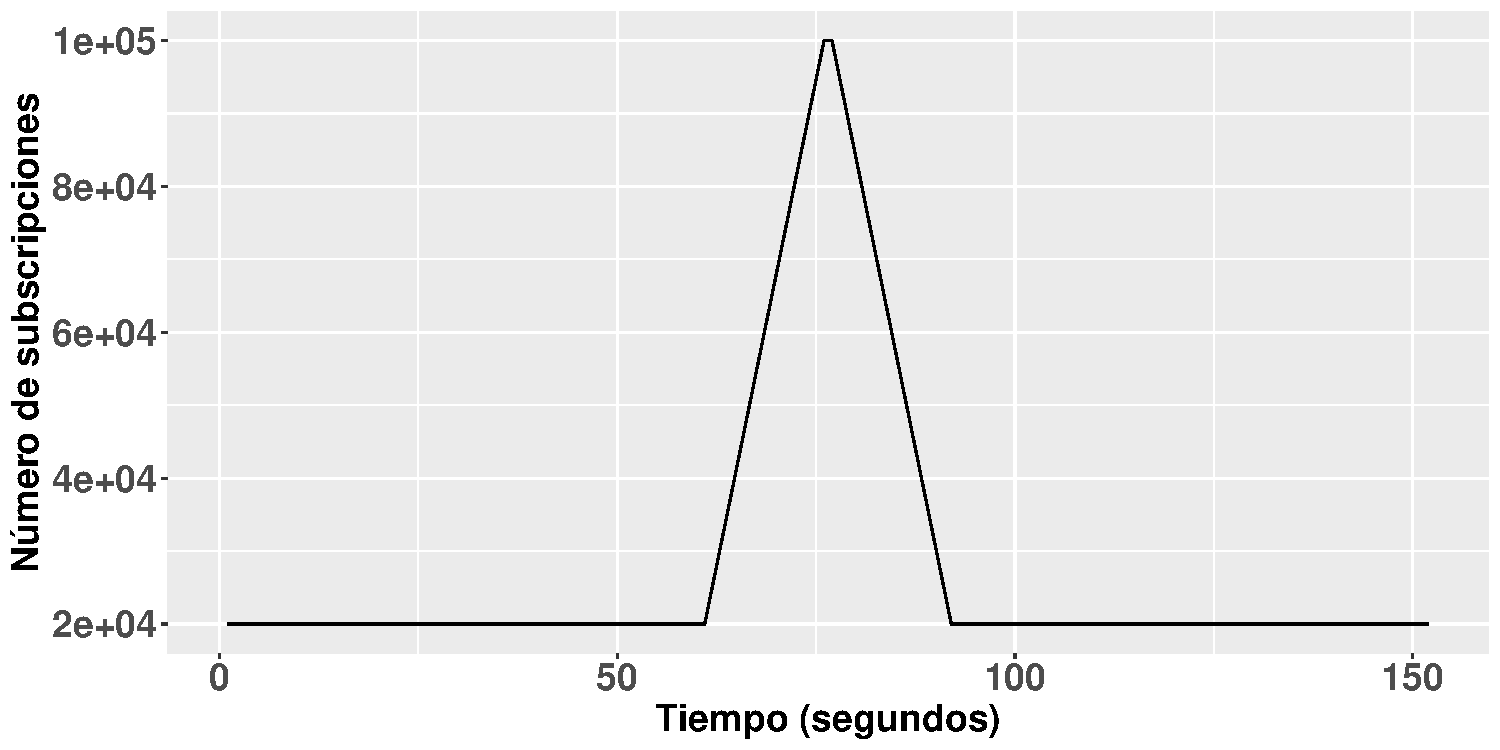
\includegraphics[width=\textwidth]{images/subs_workload_spike_20k-100k.pdf}
    \caption{Carga base de 20.000 subscripciones con incremento hasta 100.000 subscripciones.}
    \label{fig:subsworkload_20k-100k}
\end{figure}

\begin{figure}[htpb]
    \centering
    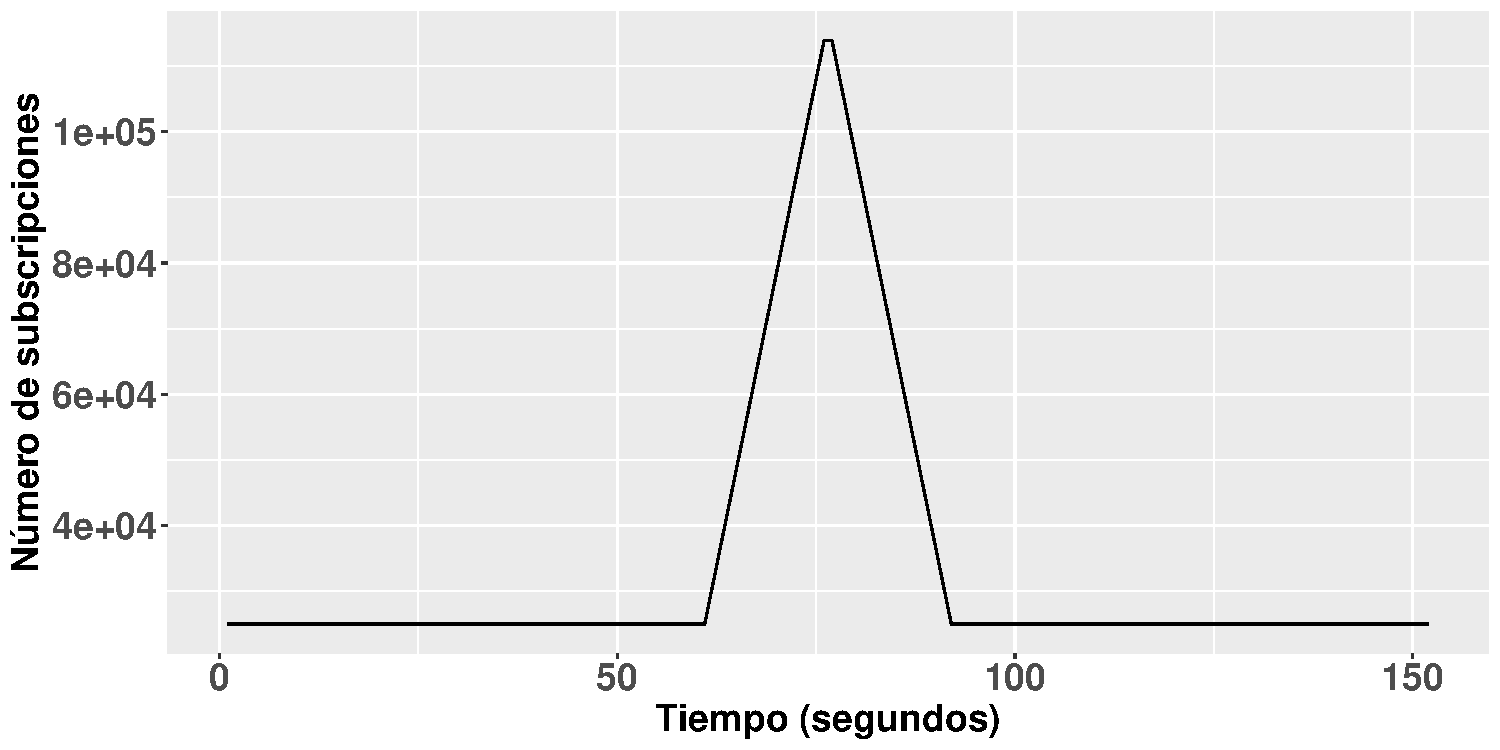
\includegraphics[width=\textwidth]{images/subs_workload_spike_25k-113k.pdf}
    \caption{Carga base de 25.000 subscripciones con incremento hasta 113.904 subscripciones.}
    \label{fig:subsworkload_25k-113k}
\end{figure}

\begin{figure}[htpb]
    \centering
    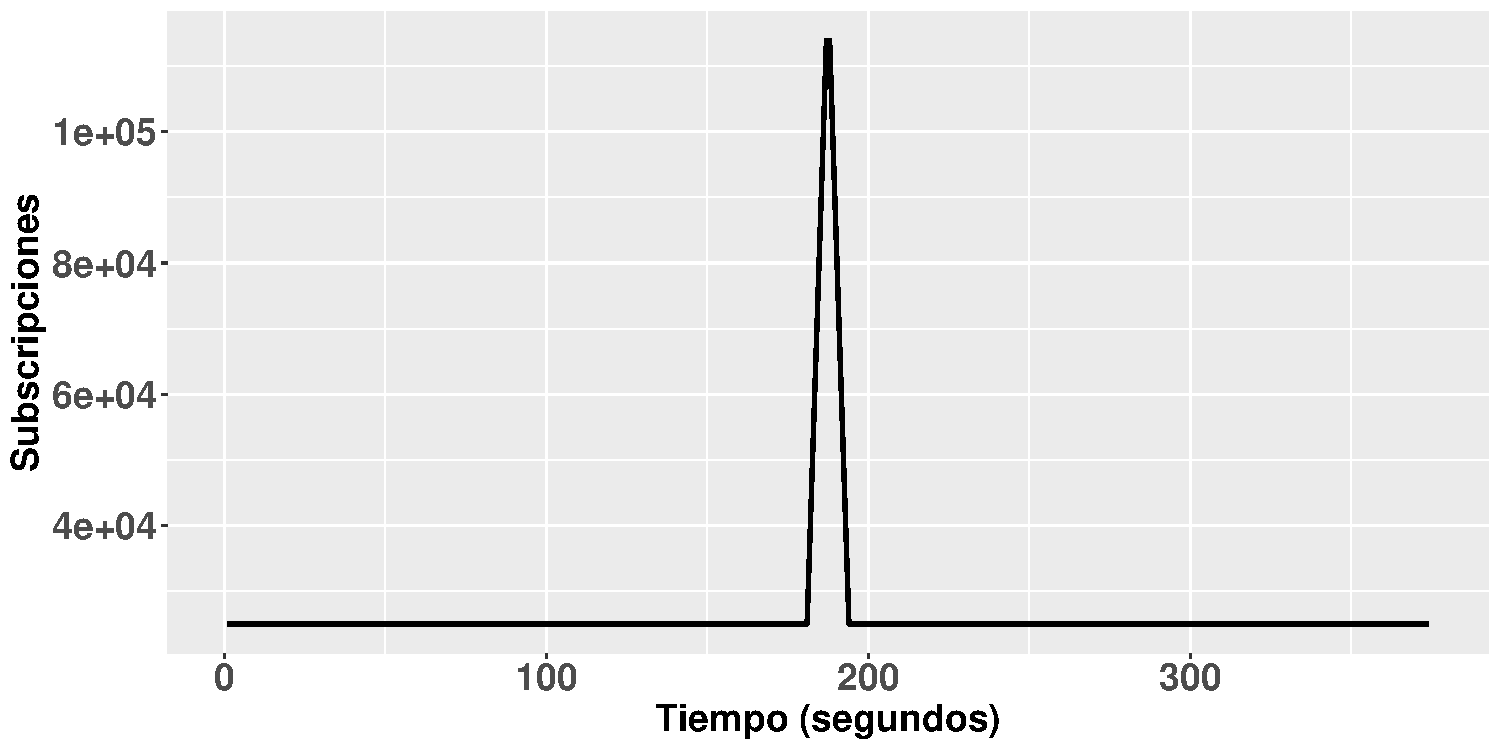
\includegraphics[width=\textwidth]{images/subs_workload_test_spike_fast_25k-113k.pdf}
    \caption{Carga base de 25.000 subscripciones con incremento muy rápido hasta 113.904 subscripciones.}
    \label{fig:subsworkload_fast_spike_25k-113k-100k}
\end{figure}



%%%%%%%%%%%%%%%%%%%%%%%%%%%%%%%%%%%%%%%%%%%%%%%%%%%%%%%%%%%%%%%%%%%%%%%%%%%%%%%%
%%%%%%%%%%%%%%%%%%%%%%%%%%%%%%%%%%%%%%%%%%%%%%%%%%%%%%%%%%%%%%%%%%%%%%%%%%%%%%%%

\section{Métricas de rendimiento} \label{sct:desarrollo_metricas}

Para poder cuantificar y analizar el rendimiento del sistema, como se ha mencionado previamente, 
es necesario obtener las principales métricas de rendimiento, con el objetivo de identificar posibles 
problemas o ineficiencias en el sistema.

Estas métricas son:
\begin{itemize}

    \item \textbf{Tiempo de respuesta} (\textit{response time}): lapso de tiempo
    desde que se envía la publicación hasta que es recibida por un usuario 
    interesado en ella.

    \item \textbf{Notificaciones enviadas a usuarios por segundo}
    (\textit{throughput}): número de notificaciones, por segundo, que han salido
    del sistema hacia usuarios interesados en ellas

\end{itemize}

Para obtener estos datos, las pruebas implementadas en la 
\autoref{sct:desarrollo_pruebas-esilbops} han recogido los tiempos de envío y 
recepción de cada mensaje, mediante los cuales se han calculado los tiempos de 
respuesta de cada publicación (que ha llegado a algún subscriptor), y el número
de mensajes totales del sistema, plasmando esta información en ficheros con el 
formato \textit{CSV}\footnote{Comma-Separated Values} para poder dibujar 
gráficas y obtener conclusiones de las pruebas y del sistema.

%%%%%%%%%%%%%%%%%%%%%%%%%%%%%%%%%%%%%%%%%%%%%%%%%%%%%%%%%%%%%%%%%%%%%%%%%%%%%%%%
%%%%%%%%%%%%%%%%%%%%%%%%%%%%%%%%%%%%%%%%%%%%%%%%%%%%%%%%%%%%%%%%%%%%%%%%%%%%%%%%

\section{Análisis de los resultados} \label{sct:desarrollo_resultados}

Con los datos obtenidos por medio de las pruebas implementadas y ejecutadas en la 
\autoref{sct:desarrollo_pruebas-esilbops}, se han obtenido los siguientes datos y 
gráficas\footnote{Ejes Y en escala logarítmica para mejor representación de los datos.}.

%%%%%%%%%%%%%%%%%%%%%%%%%%%%%%%%%%%%%%%%%%%%%%%%%%%%%%%%%%%%%%%%%%%%%%%%%%%%%%%%

\subsection*{Velocidad fija de envío}

Esta prueba, como se ha mencionado en la \autoref{ssct:desarrollo_pruebas-esilbops_test-fixed},
se ha llevado a cabo múltiples veces a diferentes velocidades de envío (input rate), para poder
ver el comportamiento del sistema, tanto en throughput como en tiempo de respuesta de notificación.

%%%%%%%%%%%%%%%%%%%%%%%%%%%%%%%%%%%%%%%%%%%%%%%%%%%%%%%%%%%%%%%%%%%%%%%%%%%%%%%%

\subsubsection*{- 50.000 mensajes por segundo}

Los resultados de esta prueba, tanto del throughput (ver 
\autoref{fig:fullworkload-inc-msgrate-th-50k}) como del 
tiempo de respuesta (ver \autoref{fig:fullworkload-inc-msgrate-rt-50k}) 
muestran un sistema que funciona sin saturar, pues el tiempo de respuesta es 
muy cercano a 0. 
El throughput muestra ciertos picos precedidos de valles, los cuales se deben 
al propio contenido de la carga de trabajo ya que hay zonas que provocan más 
subscripciones que otras, y no llega a las 50.000 notificaciones por segundo
(salvo en los ya mencionados picos), debido a que no todas las publicaciones 
producen alguna notificación.

Conclusiones de la prueba
\begin{itemize}
    \item Tiempo de respuesta mínimo y estable
    \item Throughput por debajo del input rate (esperable), picos debidos a la propia carga.
\end{itemize}

\begin{figure}[htpb]
    \centering
    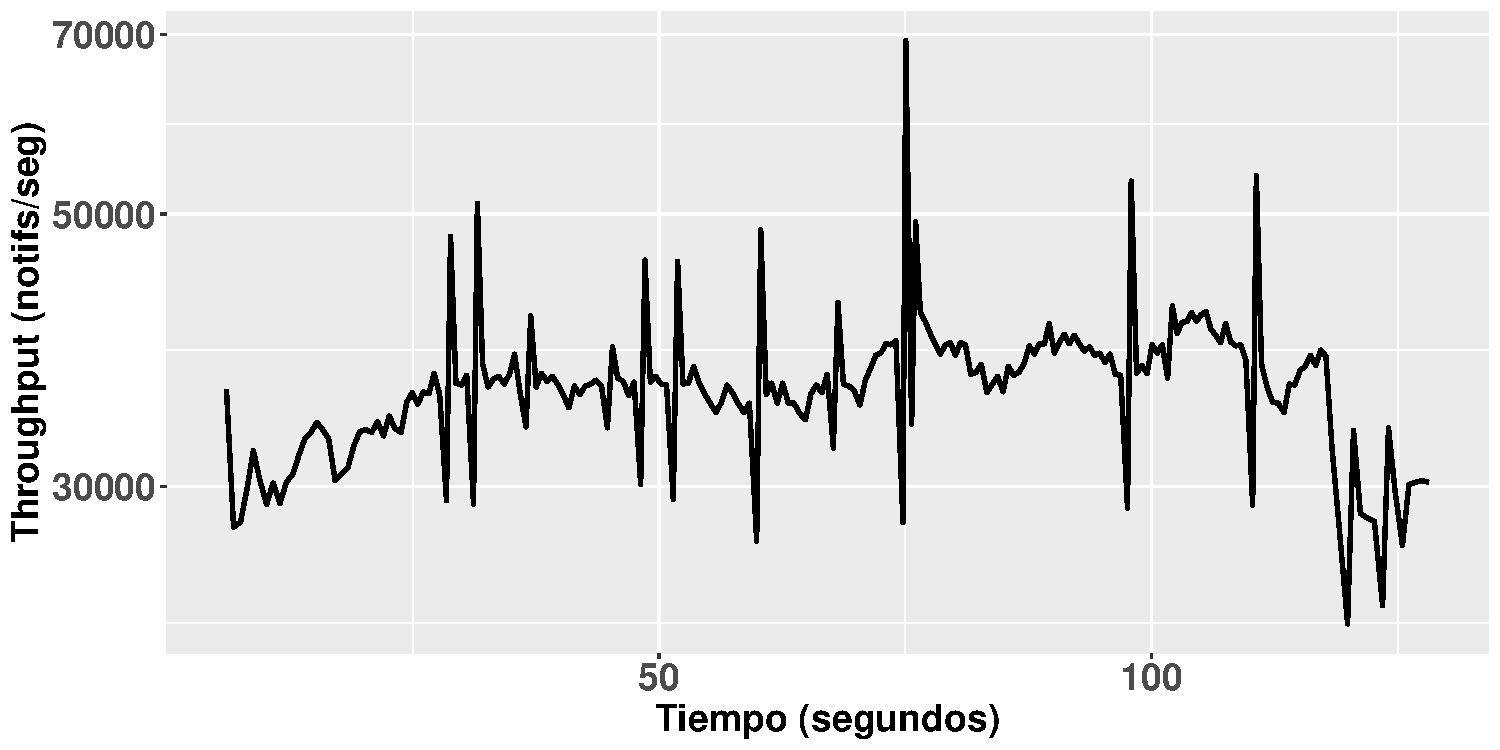
\includegraphics[width=\textwidth]{images/full-worklad-inc-msgrate/th_full-workload-inc-msgrate_50k.pdf}
    \caption{Throughput de prueba con carga completa e input rate de 50.000 mensajes/s.}
    \label{fig:fullworkload-inc-msgrate-th-50k}
\end{figure}

\begin{figure}[htpb]
    \centering
    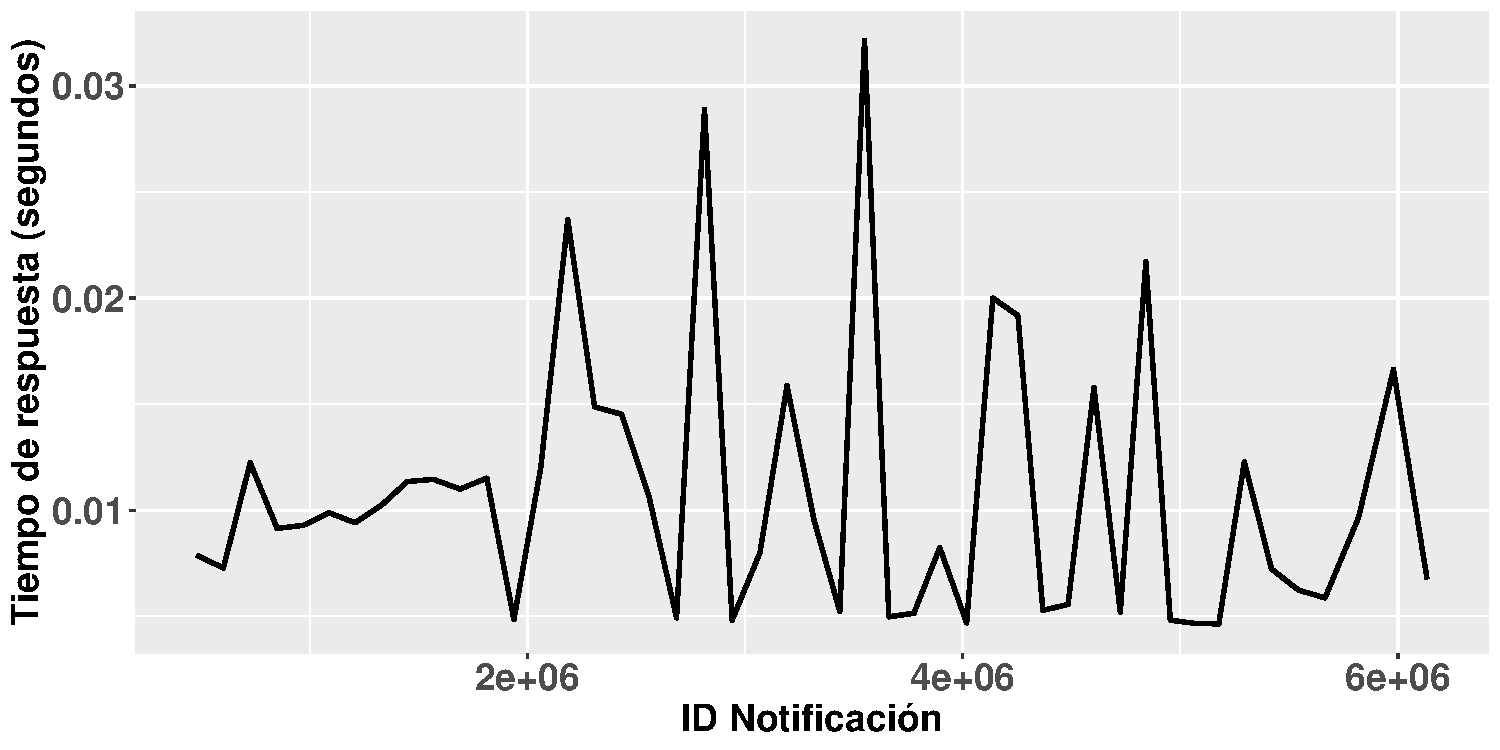
\includegraphics[width=\textwidth]{images/full-worklad-inc-msgrate/rt_full-workload-inc-msgrate_50k.pdf}
    \caption{Tiempo de respuesta de prueba con carga completa e input rate de 50.000 mensajes/s.}
    \label{fig:fullworkload-inc-msgrate-rt-50k}
\end{figure}

%%%%%%%%%%%%%%%%%%%%%%%%%%%%%%%%%%%%%%%%%%%%%%%%%%%%%%%%%%%%%%%%%%%%%%%%%%%%%%%%

\subsubsection*{- 100.000 mensajes por segundo}

Los resultados de esta prueba, tanto en el throughput (ver 
\autoref{fig:fullworkload-inc-msgrate-th-100k}) como en el tiempo de respuesta
(ver \autoref{fig:fullworkload-inc-msgrate-rt-100k}), muestran que el sistema ha
saturado de forma parcial, ya que el throughput cae muy por debajo del valor
esperado, y el tiempo de respuesta crece de forma constante, lo que indica que
el sistema no está procesando las publicaciones a tiempo, y se están encolando.

Además de esto, se puede ver claramente la relación entre ambas mediciones,
ya que la caída del throughput (\autoref{fig:fullworkload-inc-msgrate-th-100k},
a los 50 segundos), concuerda con el incremento en el tiempo de respuesta
(\autoref{fig:fullworkload-inc-msgrate-rt-100k} a partir de la notificación
con ID 3.000.000).

Conclusiones de la prueba:
\begin{itemize}
    \item El tiempo de respuesta crece de forma constante, ya que se encolan las
    notificaciones.
    \item El sistema satura de forma parcial, debido al throughput inestable, llegando
    a caer hasta los 3.000 mensajes por segundo.
\end{itemize}

\begin{figure}[htpb]
    \centering
    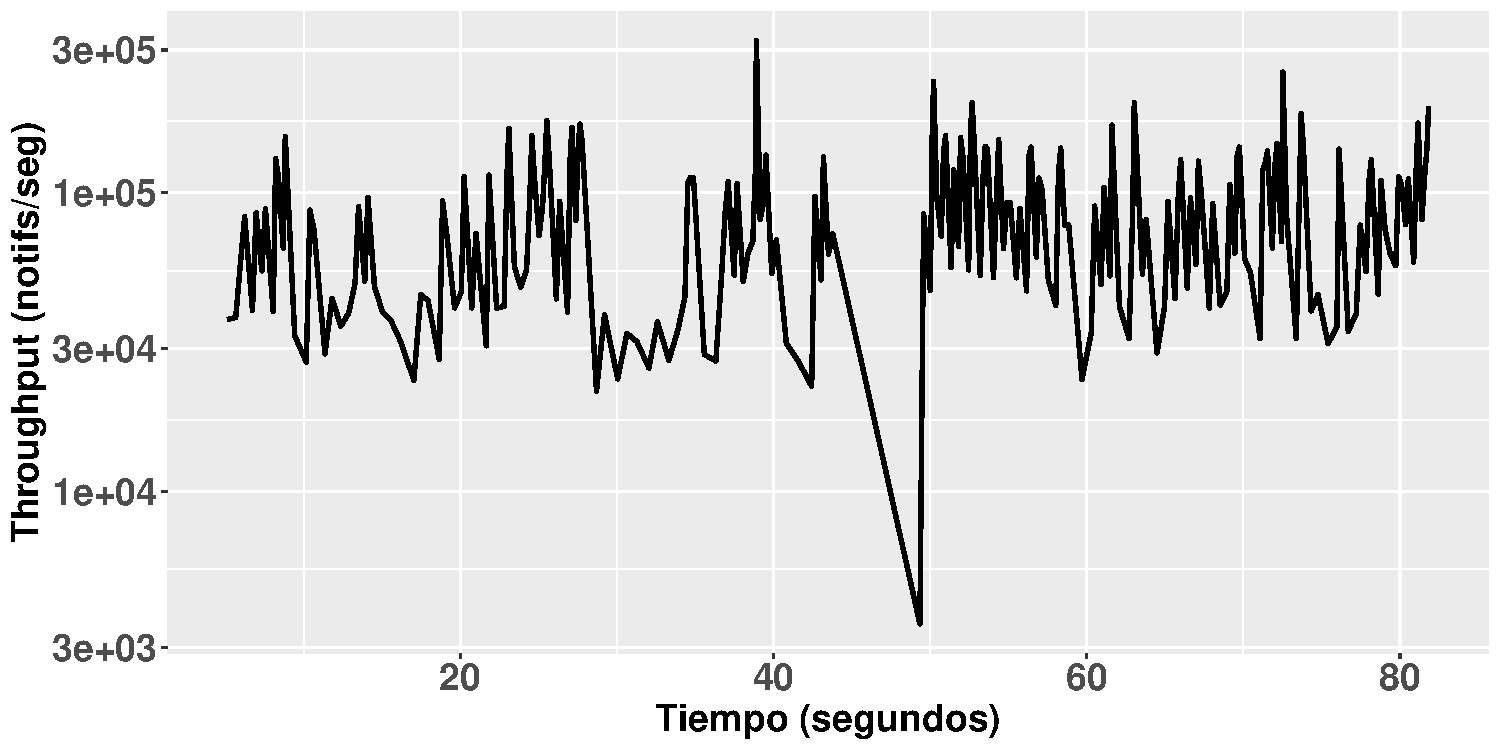
\includegraphics[width=\textwidth]{images/full-worklad-inc-msgrate/th_full-workload-inc-msgrate_100k.pdf}
    \caption{Throughput de prueba con carga completa e input rate de 100.000 mensajes/s.}
    \label{fig:fullworkload-inc-msgrate-th-100k}
\end{figure}

\begin{figure}[htpb]
    \centering
    \includegraphics[width=\textwidth]{images/full-worklad-inc-msgrate/rt_full-workload-inc-msgrate_100k.pdf}
    \caption{Tiempo de respuesta de prueba con carga completa e input rate de 100.000 mensajes/s.}
    \label{fig:fullworkload-inc-msgrate-rt-100k}
\end{figure}

%%%%%%%%%%%%%%%%%%%%%%%%%%%%%%%%%%%%%%%%%%%%%%%%%%%%%%%%%%%%%%%%%%%%%%%%%%%%%%%%

\subsubsection*{- 200.000 mensajes por segundo}

% explicaciones
En esta prueba, los resultados del throughput (ver 
\autoref{fig:fullworkload-inc-msgrate-th-200k}) y del tiempo de respuesta (ver
\autoref{fig:fullworkload-inc-msgrate-rt-200k}, demuestran que el sistema ha 
saturado, pero su throughput no ha caído tanto como anteriormente, a diferencia
del tiempo de respuesta, que sí ha crecido en gran medida, lo cual indica que las
notificaciones se están encolando en gran medida, ya que el sistema no puede 
procesarlas a tiempo, llegando estas a llegar al cliente tras más de 40 segundos.

Conclusiones de la prueba:
\begin{itemize}
    \item El tiempo de respuesta se incrementa de forma exponencial.
    \item El throughput presenta muchos picos al encolar muchas notificaciones que
    se procesan de forma muy rápida, llegando algunos picos a superar el input rate.
\end{itemize}

\begin{figure}[htpb]
    \centering
    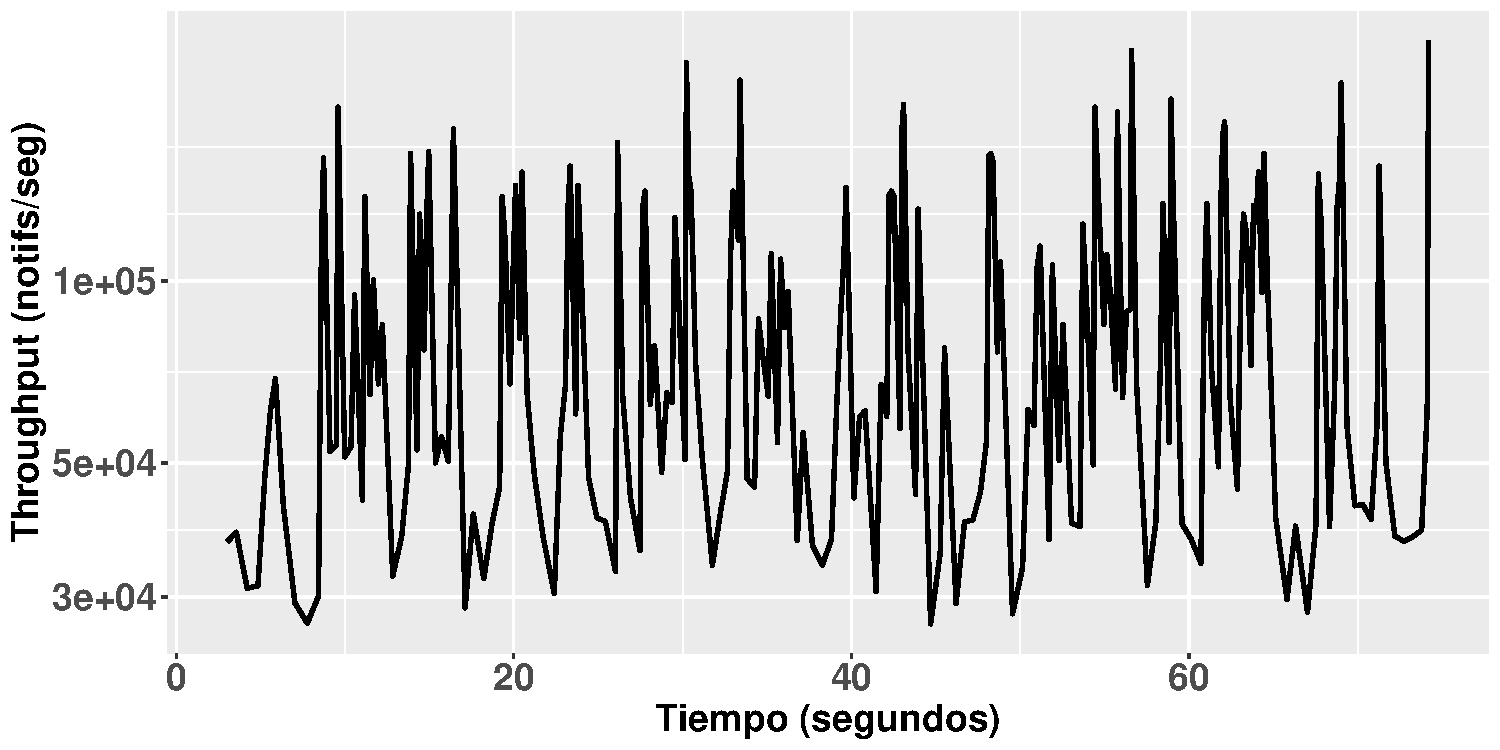
\includegraphics[width=\textwidth]{images/full-worklad-inc-msgrate/th_full-workload-inc-msgrate_200k.pdf}
    \caption{Throughput de prueba con carga completa e input rate de 200.000 mensajes/s.}
    \label{fig:fullworkload-inc-msgrate-th-200k}
\end{figure}

\begin{figure}[htpb]
    \centering
    \includegraphics[width=\textwidth]{images/full-worklad-inc-msgrate/rt_full-workload-inc-msgrate_200k.pdf}
    \caption{Tiempo de respuesta de prueba con carga completa e input rate de 200.000 mensajes/s.}
    \label{fig:fullworkload-inc-msgrate-rt-200k}
\end{figure}

%%%%%%%%%%%%%%%%%%%%%%%%%%%%%%%%%%%%%%%%%%%%%%%%%%%%%%%%%%%%%%%%%%%%%%%%%%%%%%%%

\subsubsection*{- 500.000 mensajes por segundo}

% explicaciones
Al igual que en las pruebas anteriores, se puede ver la saturación del sistema,
tanto en el throughput (ver \autoref{fig:fullworkload-inc-msgrate-th-500k})
como en el tiempo de respuesta (ver \autoref{fig:fullworkload-inc-msgrate-rt-500k}),
presentando en el primero importantes caídas (hasta casi 3.000 de throughput),
y un tiempo de respuesta que llega a casi 70 segundos. 

En esta prueba también se puede apreciar la relación del throughput y del
tiempo de respuesta, pues este último presenta dos repentinos incrementos, los cuales
coinciden con severas caídas del throughput.

Conclusiones de la prueba:
\begin{itemize}
    \item El tiempo de respuesta es mucho mayor que en anteriores pruebas, señal
    del grado de saturación del sistema.
    \item El throughput muestra severas caídas, y oscila en torno a los 100.000
    mensajes por segundo, muy por debajo de los 500.000 de input rate.
\end{itemize}

\begin{figure}[htpb]
    \centering
    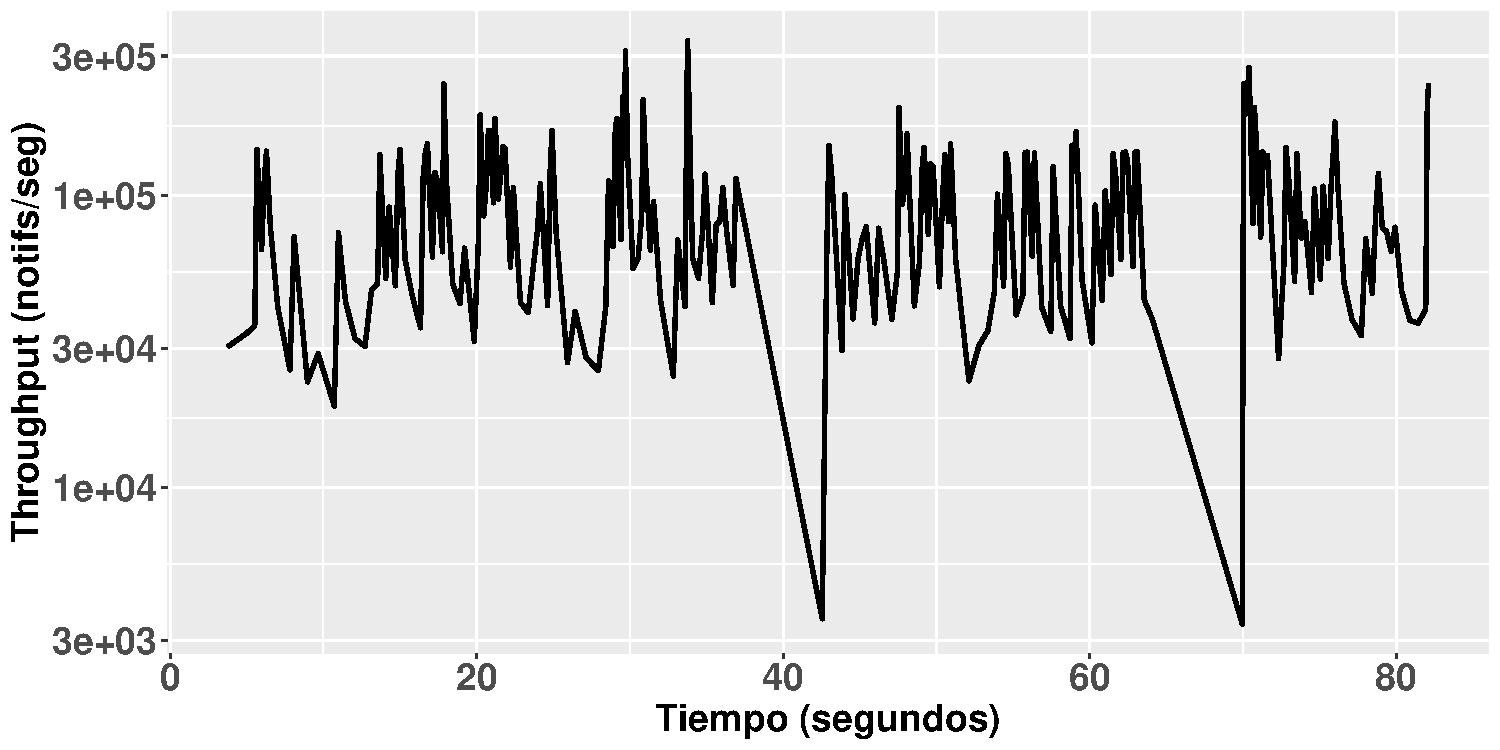
\includegraphics[width=\textwidth]{images/full-worklad-inc-msgrate/th_full-workload-inc-msgrate_500k.pdf}
    \caption{Throughput de prueba con carga completa e input rate de 500.000 mensajes/s.}
    \label{fig:fullworkload-inc-msgrate-th-500k}
\end{figure}

\begin{figure}[htpb]
    \centering
    \includegraphics[width=\textwidth]{images/full-worklad-inc-msgrate/rt_full-workload-inc-msgrate_500k.pdf}
    \caption{Tiempo de respuesta de prueba con carga completa e input rate de 500.000 mensajes/s.}
    \label{fig:fullworkload-inc-msgrate-rt-500k}
\end{figure}

%%%%%%%%%%%%%%%%%%%%%%%%%%%%%%%%%%%%%%%%%%%%%%%%%%%%%%%%%%%%%%%%%%%%%%%%%%%%%%%%

\subsubsection*{- 1.000.000 mensajes por segundo}

Los resultados de esta prueba son muy similares a los de la prueba anterior,
con un throughput (ver \autoref{fig:fullworkload-inc-msgrate-th-1M}) con muchos
picos alrededor de 75.000 mensajes por segundo, y que presenta 3 caídas severas,
las cuales coinciden con 3 incrementos presentes en el tiempo de respuesta (ver
\autoref{fig:fullworkload-inc-msgrate-rt-1M}), el cual presenta mayores valores
que en las pruebas anteriores.

Conclusiones de la prueba:
\begin{itemize}
    \item El throughput presenta serias caídas (hasta los 3.000 mensajes por segundo),
    y no llega a los 300.000 mensajes por segundo.
    \item El tiempo de respuesta denota la saturación del sistema, llegando hasta
    los 80 segundos de espera en la llegada de las notificaciones.
\end{itemize}

\begin{figure}[htpb]
    \centering
    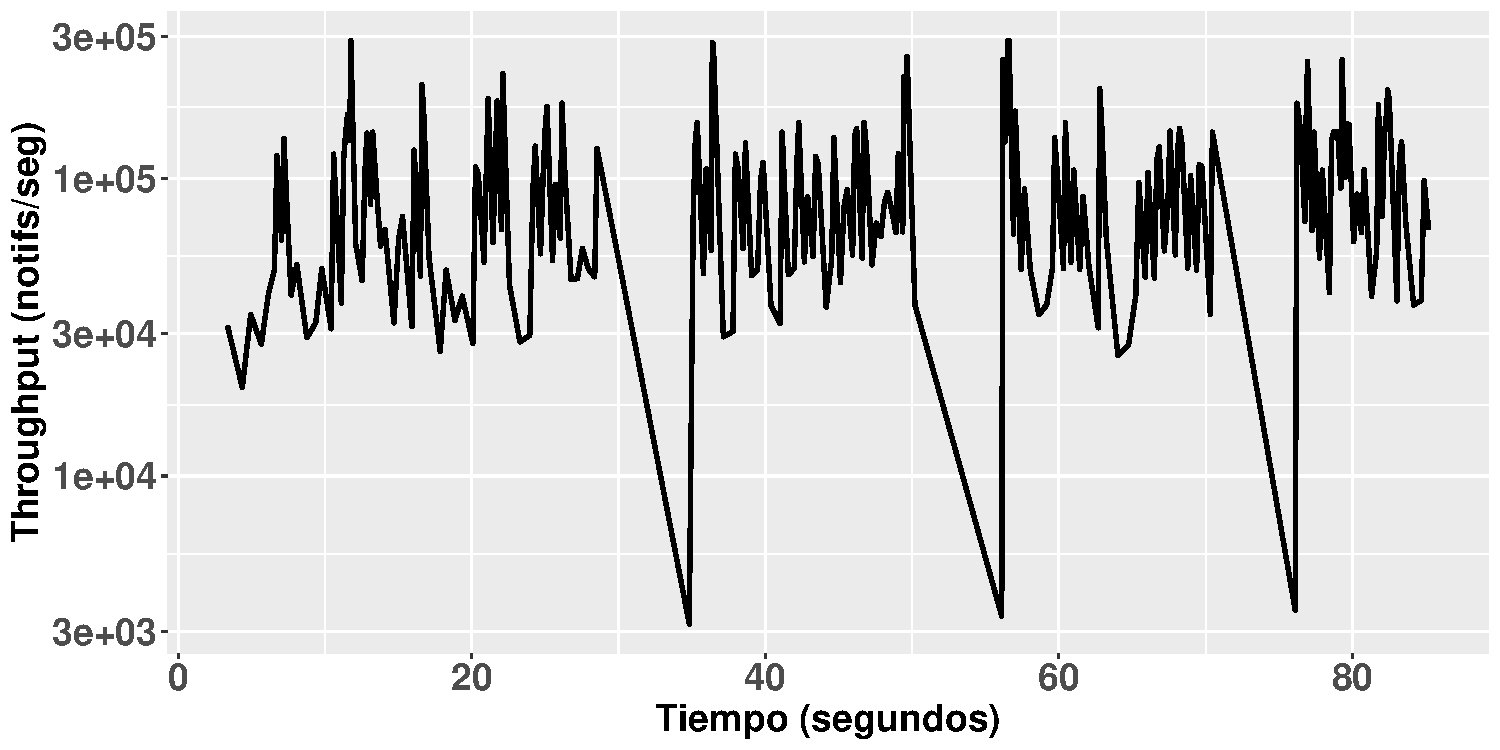
\includegraphics[width=\textwidth]{images/full-worklad-inc-msgrate/th_full-workload-inc-msgrate_1M.pdf}
    \caption{Throughput de prueba con carga completa e input rate de 1.000.000 mensajes/s.}
    \label{fig:fullworkload-inc-msgrate-th-1M}
\end{figure}

\begin{figure}[htpb]
    \centering
    \includegraphics[width=\textwidth]{images/full-worklad-inc-msgrate/rt_full-workload-inc-msgrate_1M.pdf}
    \caption{Tiempo de respuesta de prueba con carga completa e input rate de 1.000.000 mensajes/s.}
    \label{fig:fullworkload-inc-msgrate-rt-1M}
\end{figure}

%%%%%%%%%%%%%%%%%%%%%%%%%%%%%%%%%%%%%%%%%%%%%%%%%%%%%%%%%%%%%%%%%%%%%%%%%%%%%%%%

\subsubsection*{- 6.433.794 mensajes por segundo (máxima velocidad posible)}

Esta prueba presenta unos resultados similares a los resultados de las anteriores
pruebas (lo cual es esperable), con un throughput con caídas
(ver \autoref{fig:fullworkload-inc-msgrate-th-full}), que coinciden
con incrementos en el tiempo de respuesta (ver 
\autoref{fig:fullworkload-inc-msgrate-rt-full}), el cual presenta unos valores
en incremento, igual que en previas pruebas, llegando a los 85 segundos de tiempo
de respuesta.

Conclusiones de la prueba:
\begin{itemize}
    \item Viendo esta prueba y las anteriores, el throughput no supera los
    300.000, y en este caso, solo supera los 200.000 en ciertos picos, precedidos
    de valles (notificaciones encoladas que se procesan a gran velocidad).
    \item El tiempo de respuesta presenta unos valores en incremento, lo que concuerda
    con los valores del throughput, y con la propia saturación del sistema.
\end{itemize}

\begin{figure}[htpb]
    \centering
    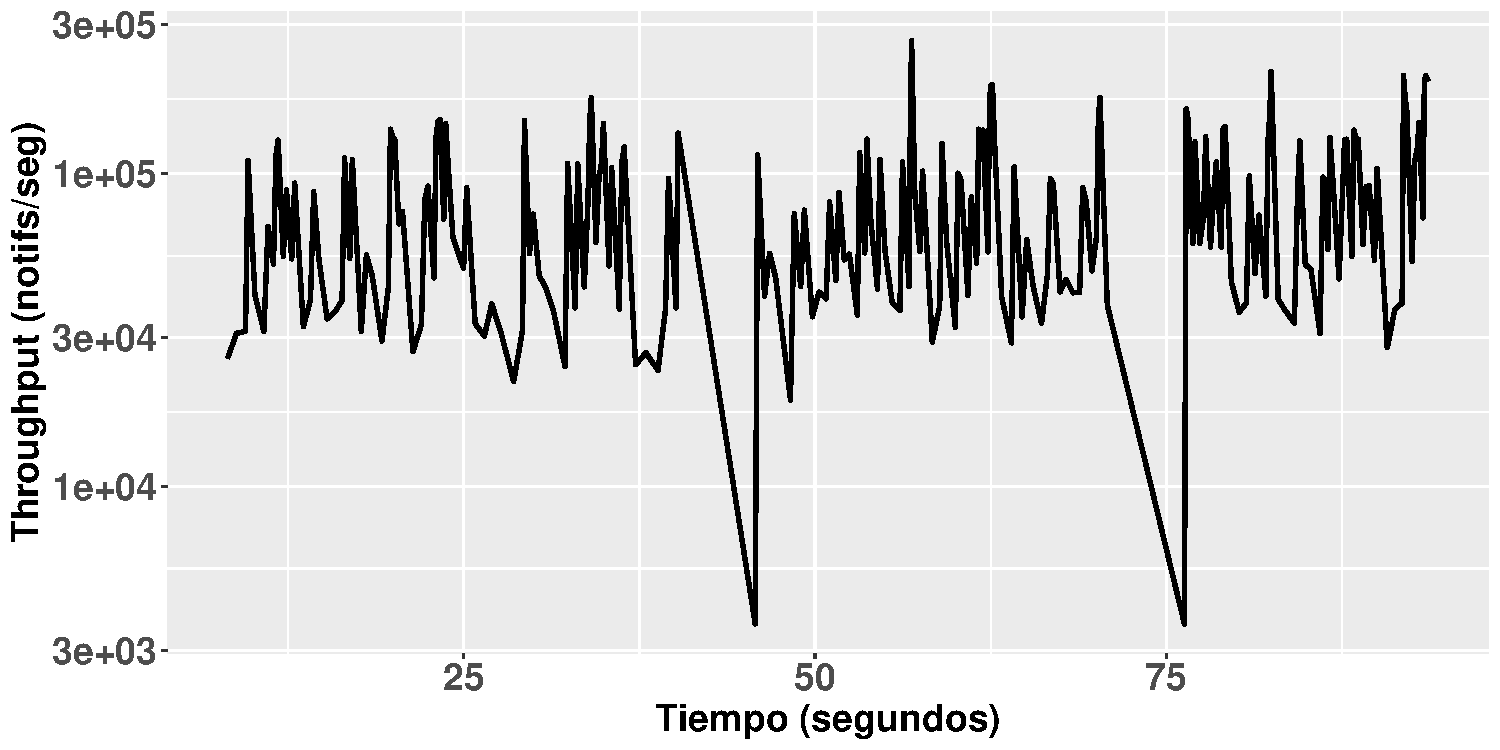
\includegraphics[width=\textwidth]{images/full-worklad-inc-msgrate/th_full-workload-inc-msgrate_full.pdf}
    \caption{Throughput de prueba con carga completa a máximo input rate.}
    \label{fig:fullworkload-inc-msgrate-th-full}
\end{figure}

\begin{figure}[htpb]
    \centering
    \includegraphics[width=\textwidth]{images/full-worklad-inc-msgrate/rt_full-workload-inc-msgrate_full.pdf}
    \caption{Tiempo de respuesta de prueba con carga completa a máximo input rate.}
    \label{fig:fullworkload-inc-msgrate-rt-full}
\end{figure}

%%%%%%%%%%%%%%%%%%%%%%%%%%%%%%%%%%%%%%%%%%%%%%%%%%%%%%%%%%%%%%%%%%%%%%%%%%%%%%%%

\subsection*{Secuencia logarítmica de subscripciones}

Como se puede observar en la \autoref{fig:throughput_logsubs}, el throughput 
del sistema decae de forma considerable pasadas las 20.000 subscripciones 
activas, ya que el tiempo invertido en comprobar todas las subscripciones 
incrementa y provoca un aumento en el tiempo de procesado de cada publicación,
en concreto, en la confección de la lista de subscripciones interesadas en
dicha publicación.

Esto indica que con la configuración actual (1-1-1), el sistema está saturando
cuando tiene que comprobar, al menos, 20.000 subscripciones. En este punto, si
estuviese activada la escalabilidad, el sistema debería de haber escalado para
no llegar a saturar.

\begin{figure}[htpb]
    \centering
    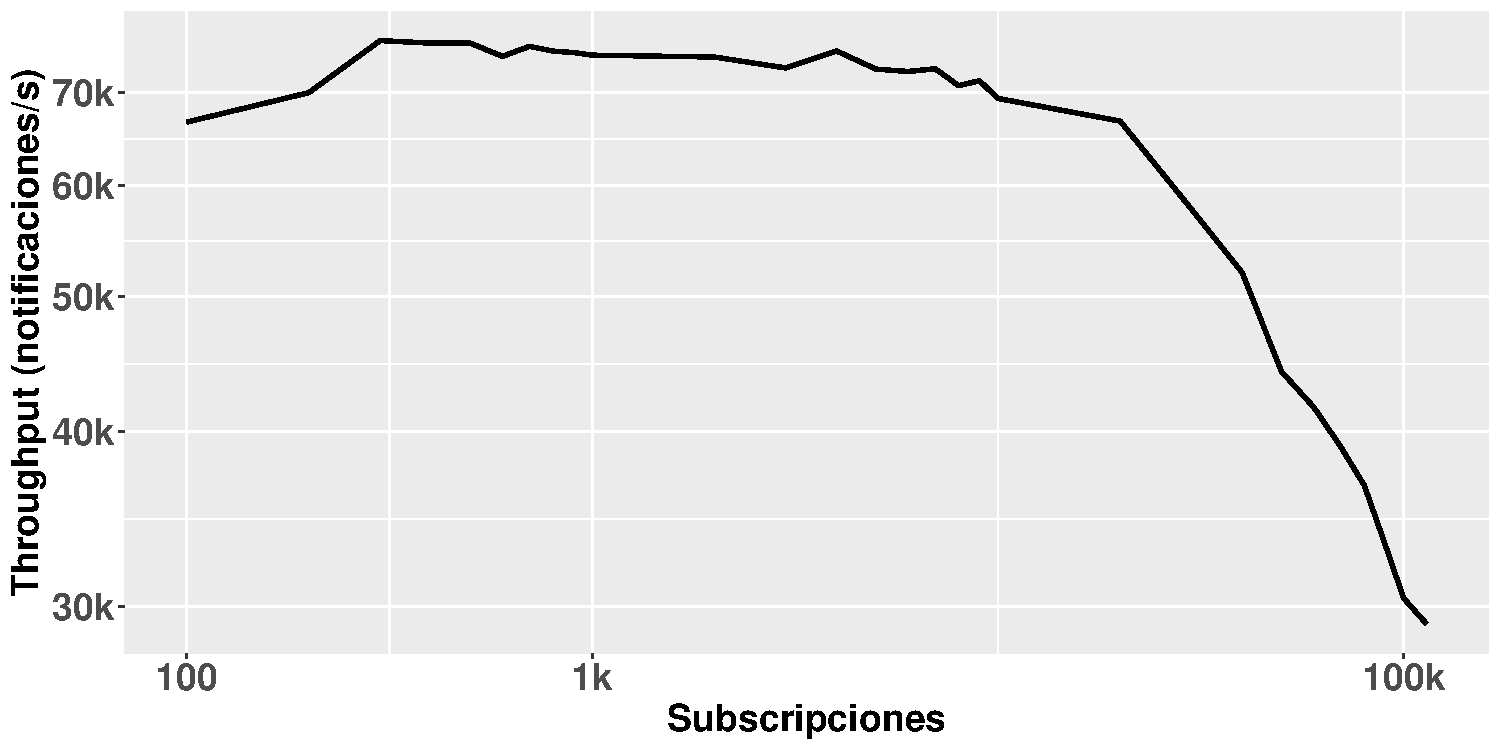
\includegraphics[width=\textwidth]{images/log-subs/throughput_logsubs_IR-100k.pdf}
    \caption{Throughput en base a la subscripciones activas con un input rate de 100.000 mensajes por segundo en ejes logarítmicos.}
    \label{fig:throughput_logsubs}
\end{figure}

Conociendo este punto de saturación, lo siguiente es probar el sistema con esa
carga de subscripciones, de forma que se vea con mayor precisión cómo actúa el
sistema con un número de subscripciones cercano al del punto de saturación.

%%%%%%%%%%%%%%%%%%%%%%%%%%%%%%%%%%%%%%%%%%%%%%%%%%%%%%%%%%%%%%%%%%%%%%%%%%%%%%%%

\subsection*{Carga de subscripciones creciente}

Como se puede observar en la \autoref{fig:throughput_incsubsload-fullpubs}, el
throughput del sistema cae en gran medida, con una media de 18.000 mensajes 
por segundo, con picos cercanos a los 30.000.

Este primer pico se debe al aumento de subscripciones, que provocan que las 
publicaciones enviadas de forma paralela generen un mayor número de notificaciones,
lo cual aumenta el número de notificaciones generadas por segundo.

De igual forma, estos picos pueden estar causados por la naturaleza de la
distribución de subscripciones y publicaciones, ya que ciertas secciones de la 
carga de publicaciones pueden generar mayor número de notificaciones, al
machear con más subscripciones activas.

A causa de esto, se requiere de realizar nuevas pruebas con otro tipo de
carga de trabajo, que pruebe la saturación del sistema con incrementos puntuales,
como se puede esperar en un contexto real.

\begin{figure}[htpb]
    \centering
    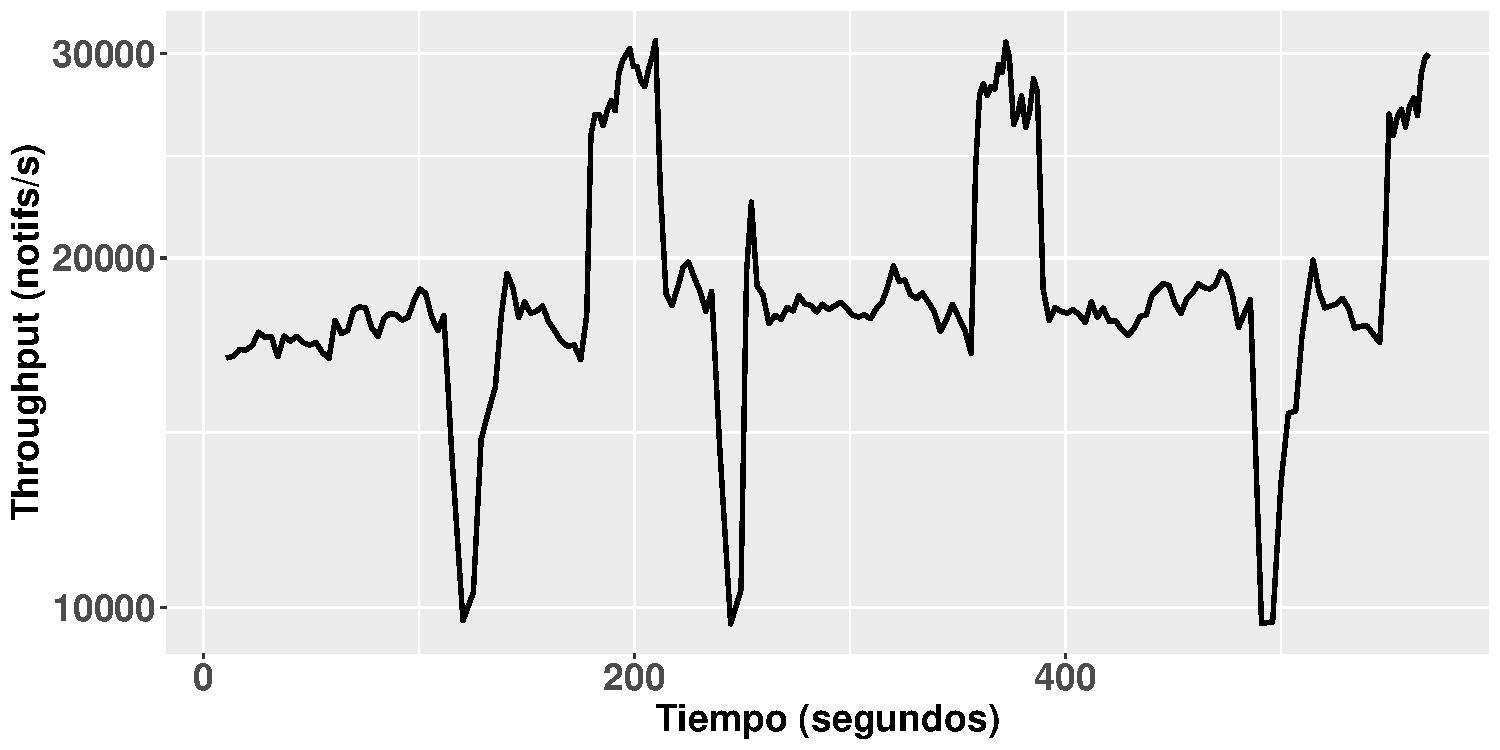
\includegraphics[width=\textwidth]{images/throughput_inc-subs-load-full.pdf}
    \caption{Throughput del sistema con la carga de subscripciones y todas las publicaciones}
    \label{fig:throughput_incsubsload-fullpubs}
\end{figure}


%%%%%%%%%%%%%%%%%%%%%%%%%%%%%%%%%%%%%%%%%%%%%%%%%%%%%%%%%%%%%%%%%%%%%%%%%%%%%%%%

\subsection*{Carga de subscripciones estática}

\subsubsection*{- 50.000 subscripciones}

En la \autoref{fig:subsworkload_50k-200k} se puede observar la caída de rendimiento
del sistema, pues ha llegado al punto de saturación parcial al caer este muy por debajo
del throughput esperado de 200.000 mensajes por segundo. Las fluctuaciones 
indican que el sistema, en ciertos momentos, encola gran cantidad de eventos, al
no poder procesarlos a tiempo, pero recupera ese tiempo perdido en los siguientes
segundos. A pesar de esto, el sistema no llega a saturar de la forma esperada, es decir,
se recupera más rápido de lo esperado, lo cual es bueno para el sistema, pero no nos 
proporciona la información buscada.

\begin{figure}[htpb]
    \centering
    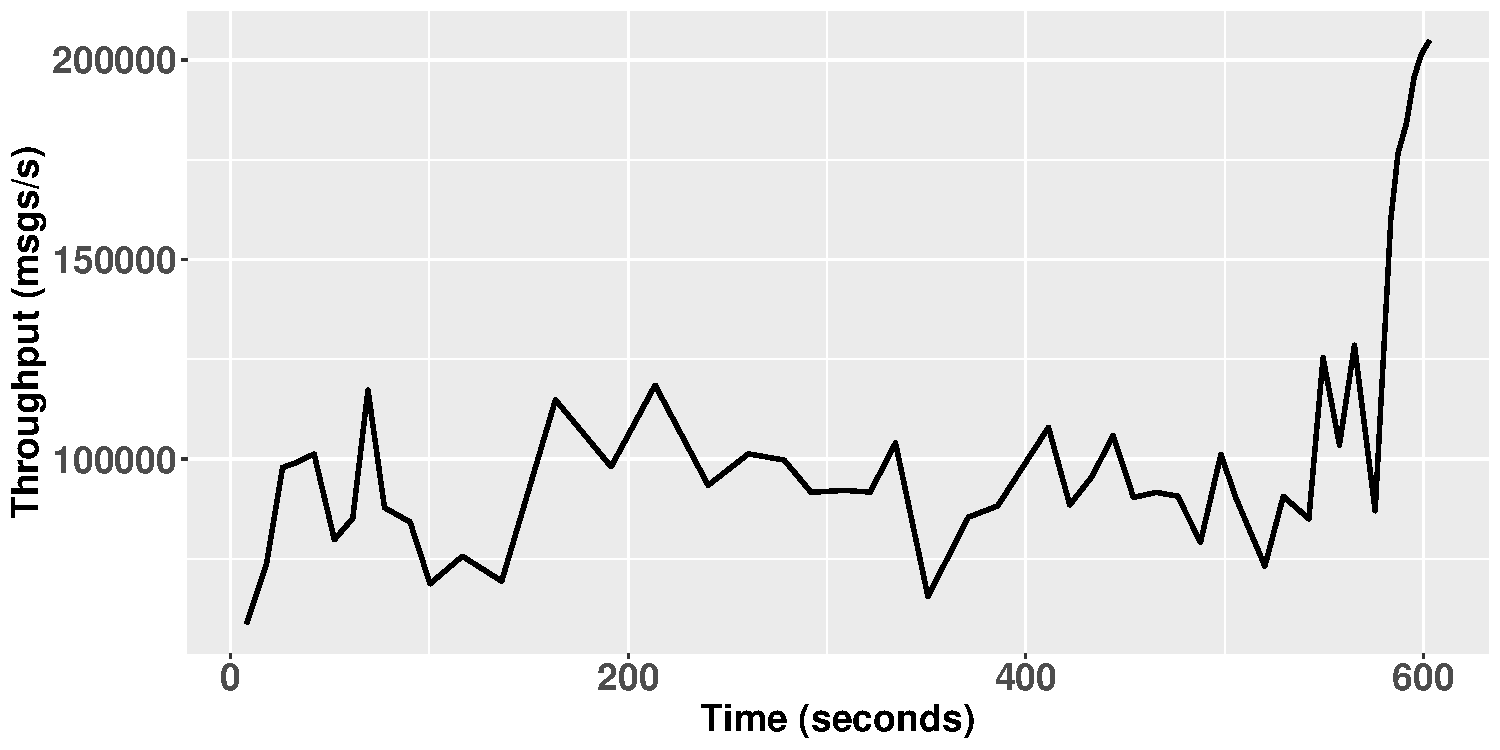
\includegraphics[width=\textwidth]{images/th_subs_workload-50k-200k.pdf}
    \caption{Throughput resultante de una prueba con 50.000 subscripciones y un input rate de 200.000 publicaciones por segundo.}
    \label{fig:subsworkload_50k-200k}
\end{figure}

\subsubsection*{- 100.000 subscripciones}

Si se lleva esta prueba al límite, es decir, el caso máximo en el cual dicha prueba puede
acabar sin quedarse el ordenador sin memoria para llevarla a cabo, se puede observar
la inestabilidad del rendimiento del sistema, al haber este saturado de forma parcial.
Esto se puede observar en la \autoref{fig:subsworkload_100k-200k}.

\begin{figure}[htpb]
    \centering
    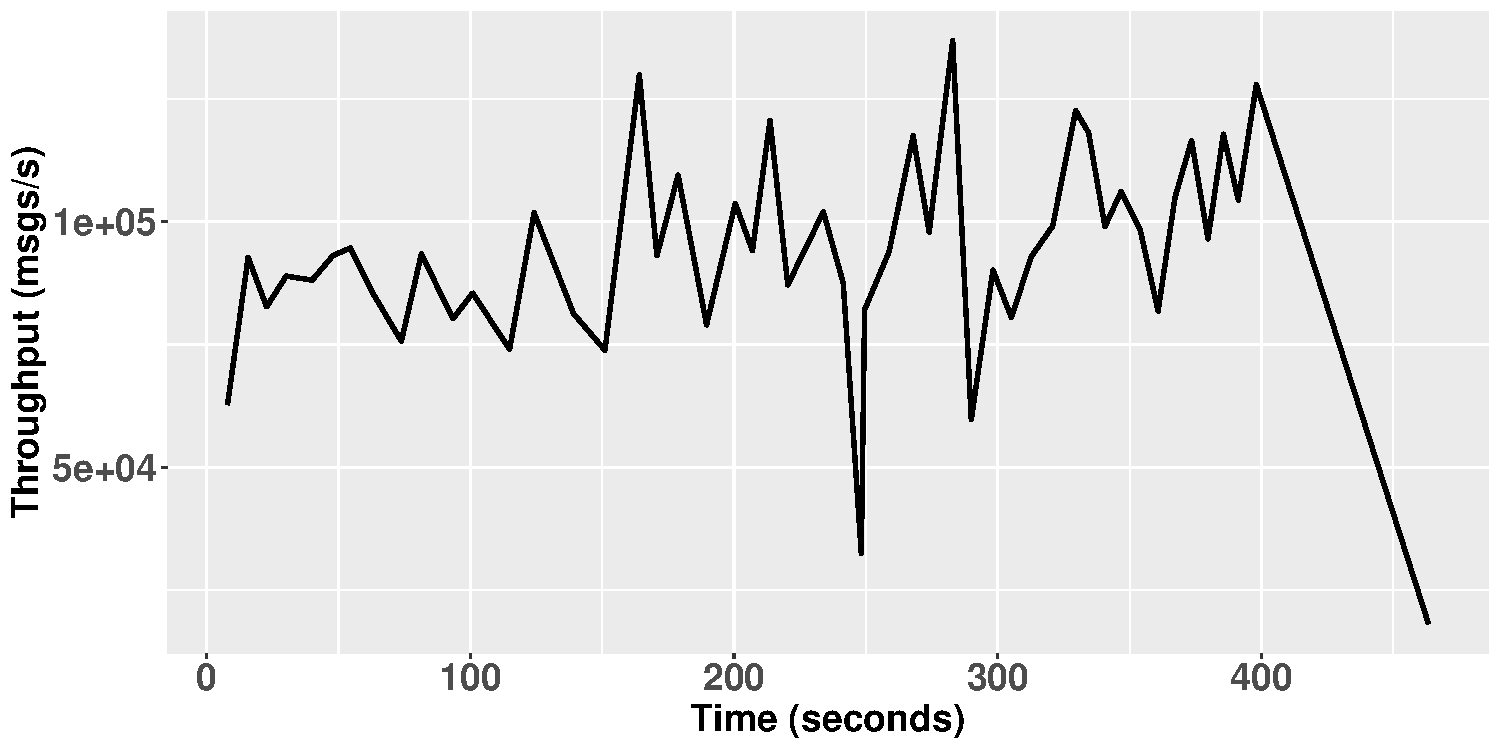
\includegraphics[width=\textwidth]{images/th_subs_workload-100k-200k.pdf}
    \caption{Throughput resultante de una prueba con 100000 subscripciones y un input rate de 200.000 publicaciones por segundo.}
    \label{fig:subsworkload_100k-200k}
\end{figure}

Los resultados obtenidos mediante estas pruebas nos muestran que el sistema satura
parcialmente de forma efectiva con una carga de 100.000 subscripciones y un input rate
mayor o igual a 150.000 mensajes por segundo. Esta respuesta nos ayuda a encontrar, con
mayor precisión, pero para ello se han de poner en práctica más pruebas con diferentes
cargas.

\subsection*{Carga de subscripciones con crecimiento puntual}

\subsubsection*{Crecimiento de 20.000 a 100.000 subscripciones}

Siguiendo el modelo de pruebas previamente empleado, mediante aplicar carga 
representada por la \autoref{fig:subsworkload_20k-100k}, y especificando un 
input rate fijo de 125.000 mensajes por segundo, se ha obtenido el throughput
que se muestra en la \autoref{fig:subsworkload_spike_20k-100k-125k}.

\begin{figure}[htpb]
    \centering
    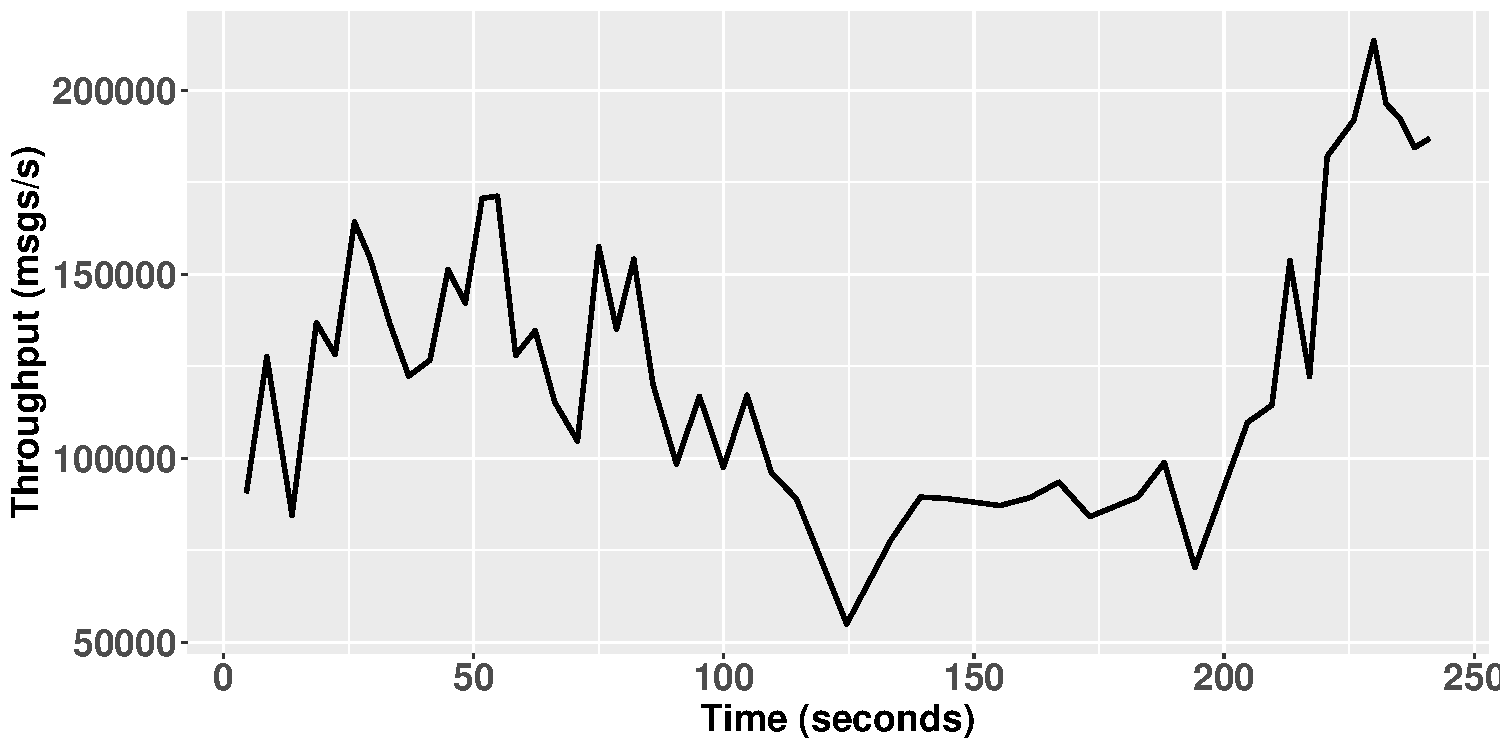
\includegraphics[width=\textwidth]{images/throguhput_spike_20k-100k-125k.pdf}
    \caption{Throughput resultante de la carga de la \autoref{fig:subsworkload_20k-100k} e input rate de 125.000 publicaciones por segundo.}
    \label{fig:subsworkload_spike_20k-100k-125k}
\end{figure}

El throughput de la \autoref{fig:subsworkload_spike_20k-100k-125k} demuestra que
el sistema ha saturado parcialmente, y ha llegado a recuperarse en la segunda mitad
de la prueba, llegando a un throughput de 125.000, al haber encolado gran cantidad de
mensajes. Junto con esto, se aprecia un throughput muy inestable, con muchos picos
bajos y altos. Los valores proporcionados para esta prueba son los más altos posibles,
sin que la ordenador se quede sin memoria para poder llevar a cabo esta, por lo que
sabemos que el sistema satura de forma efectiva a partir de estos valores.

\subsubsection*{Crecimiento de 25.000 a 100.000 subscripciones}

A raíz de estos resultados, se ha desarrollado la carga representada por la 
\autoref{fig:subsworkload_25k-113k} que resulta en el throughput representado por 
la \autoref{fig:subsworkload_spike_25k-113k-125k}.

\begin{figure}[htpb]
    \centering
    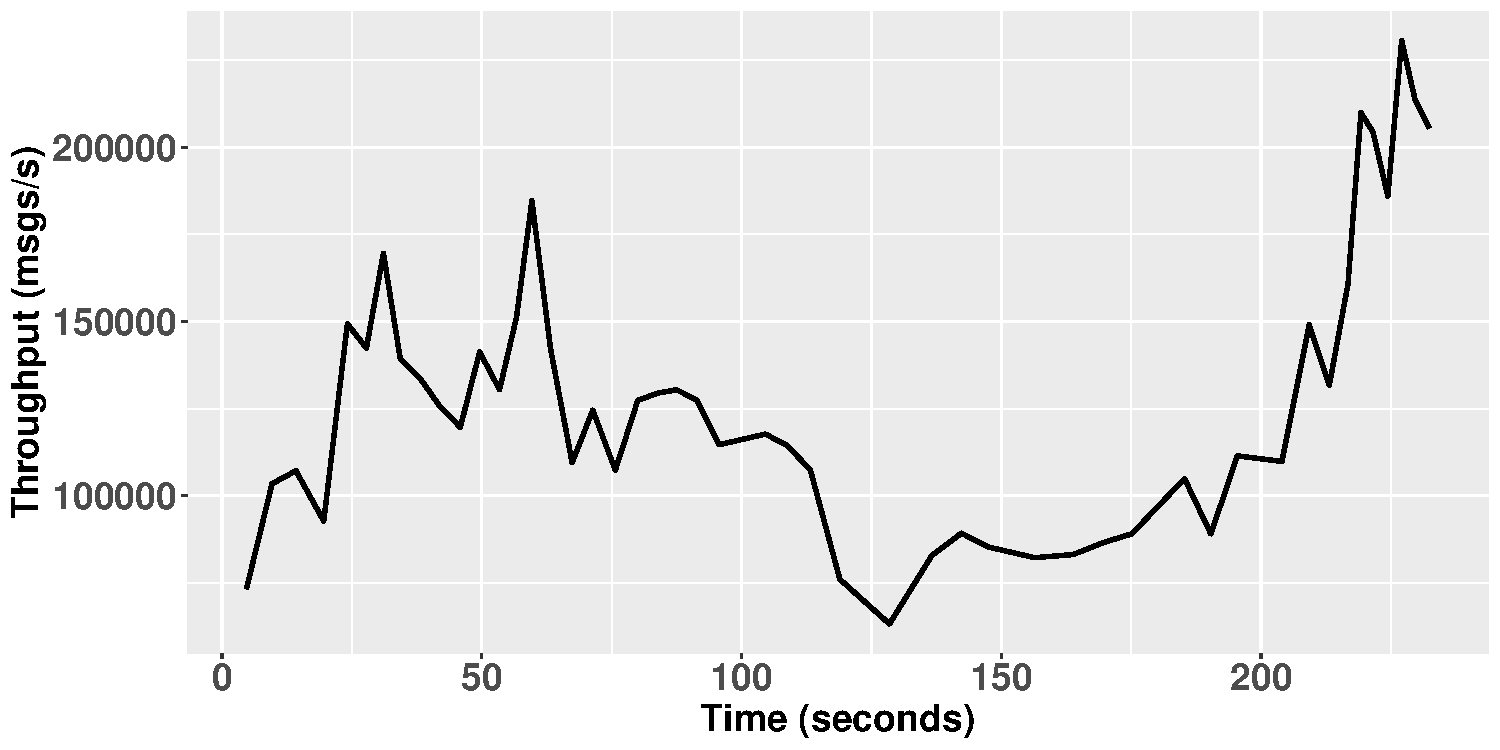
\includegraphics[width=\textwidth]{images/throguhput_spike_20k-113k-125k.pdf}
    \caption{Throughput resultante de la carga de la \autoref{fig:subsworkload_25k-113k} e input rate de 125.000 publicaciones por segundo.}
    \label{fig:subsworkload_spike_25k-113k-125k}
\end{figure}

Dados estos resultados, el comportamiento del sistema con estas pruebas no es el óptimo
para aplicar estos valores a los modelos predictivos. A causa de esto, se ha desarrollado
una prueba adicional, similar a las anteriores, pero que implementa un incremento más
repentino (llegar al máximo en 2-3 segundos) con un menor input ratio, de forma que el
sistema sature parcialmente en el punto del incremento, pero sea capaz de recuperarse
a tiempo.

\subsubsection*{Crecimiento rápido de 25.000 a 113.904 subscripciones}

Los resultados de esta prueba, que sigue los mismos parámetros que la anterior pero con un
input ratio de 100.000 mensajes por segundo, se pueden observar en la
\autoref{fig:subsworkload_th_fast_spike_25k-113k-100k}, que muestra una saturación muy leve del
sistema cuando se alcanza el incremento de la carga, pero en sistema se recupera en muy poco tiempo.

Este resultado, a pesar de haber saturado de forma mínima el sistema, es el buscado, pues el
throughput del sistema es estable y el sistema satura de la forma esperada, a pesar de haberse
recuperado rápidamente.

\begin{figure}[htpb]
    \centering
    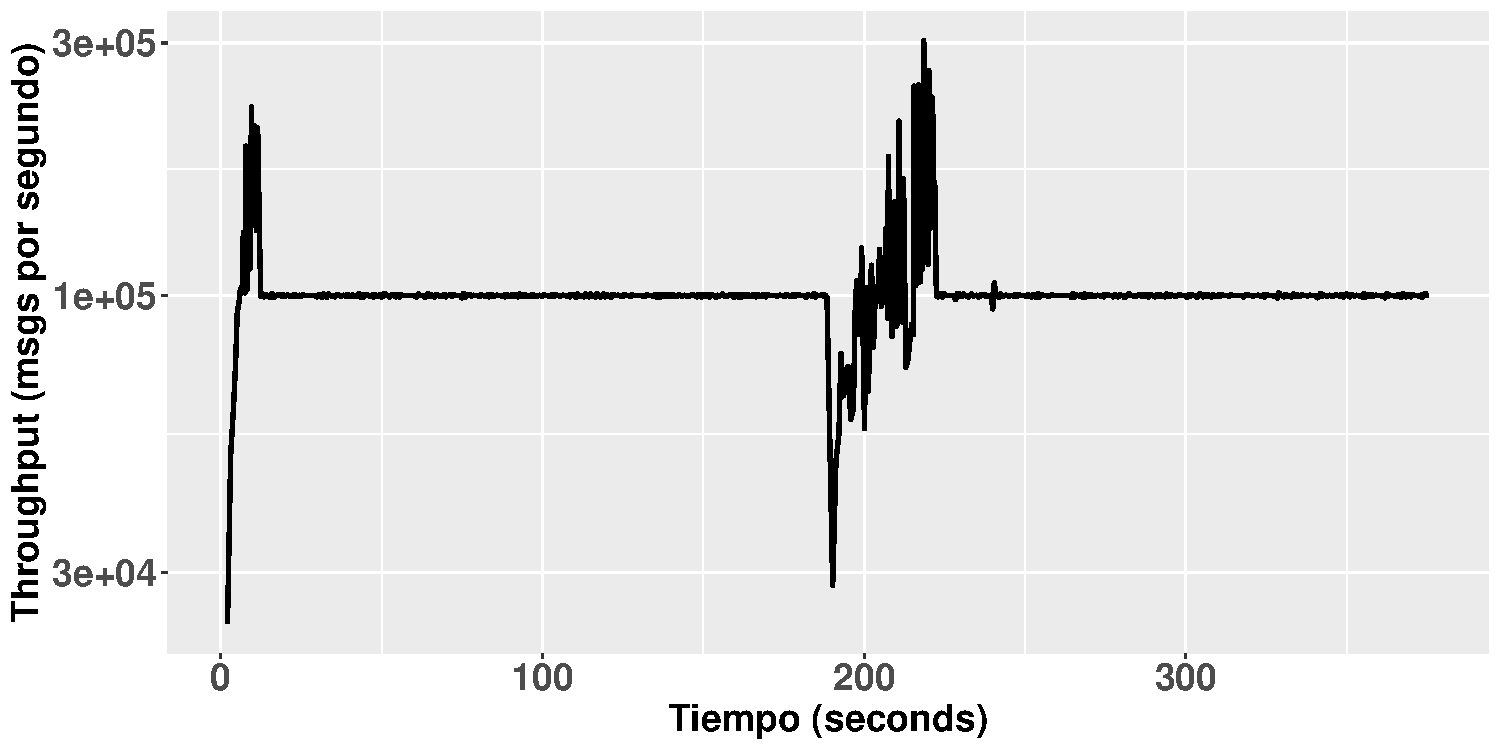
\includegraphics[width=\textwidth]{images/th_test_spike_25k-113k_100000.pdf}
    \caption{Throughput resultante de la carga de la \autoref{fig:subsworkload_fast_spike_25k-113k-100k} e input rate de 100.000 publicaciones por segundo.}
    \label{fig:subsworkload_th_fast_spike_25k-113k-100k}
\end{figure}

Habiendo obtenido estos resultados, que simulan diferentes situaciones
reales, podemos usar estos para aplicar los modelos predictivos, una vez
desarrollados e implementados estos. Los modelos predictivos usarán estos 
resultados para llevar a cabo dichas predicciones, para que el sistema pueda
anticiparse a cualquier situación que sea posible predecir.
\chapter{Generación de modelos predictivos para el auto-escalado de E-SilboPS} \label{chp:modelos}


En este capítulo, se aborda la generación de los modelos predictivos, mediante
la implementación de algoritmos de Machine-Learning y Deep-Learning, que 
usarán los resultados de las pruebas de rendimiento para predecir el 
comportamiento del sistema.

%%%%%%%%%%%%%%%%%%%%%%%%%%%%%%%%%%%%%%%%%%%%%%%%%%%%%%%%%%%%%%%%%%%%%%%%%%%%%%%%
%%%%%%%%%%%%%%%%%%%%%%%%%%%%%%%%%%%%%%%%%%%%%%%%%%%%%%%%%%%%%%%%%%%%%%%%%%%%%%%%

\section{Modelos predictivos} \label{sct:modelos_modelos-pred}
% Explicar los modelos y qué hacen

Además de estos modelos, también se ha implementado la capacidad de calcular
la primera derivada de los resultados de los modelos, pudiendo obtener resultados
más detallados.

\subsection{Métodos de Series Temporales}

Los primeros modelos que se han implementado han sido los de Series Temporales,
que hacen uso de ''Rolling Forecasting Origin''\cite{web:caret} para ajustar dichos
modelos y poder realizar predicciones.

Para comprobar los resultados de estos modelos, se comparan los valores de la
predicción con todos los anteriores, no solo con el inmediatamente anterior, lo
que lleva a un mejor ajuste de estos modelos al aumentar la precisión de dichas 
predicciones.

\subsubsection*{Rolling Forecasting Origin}

Este método permite dividir una serie de datos temporales en dos series de datos,
una de entrenamiento, y otra de pruebas, de forma que los modelos se puedan ajustar 
con la primera, y se prueben con la segunda.

Esta división se lleva a cabo mediante especificar el tamaño inicial de cada serie,
es decir, el número de valores de la serie temporal que se usarán de forma inicial;
y variando el horizonte, que es el número valores consecutivos en la serie de prueba.

De esta forma, y mediante el tamaño inicial, se establecen el número de repeticiones
de este método (''resampling''), aumentando/moviendo las series temporales de 
entrenamiento y pruebas, tal como se ve en la \autoref{fig:models_time-series}.

Adicionalmente, se puede establecer que la serie de entrenamiento añada los nuevos
valores a los anteriores, de forma que esta crezca con cada repetición.

\begin{figure}[htpb]
    \centering
    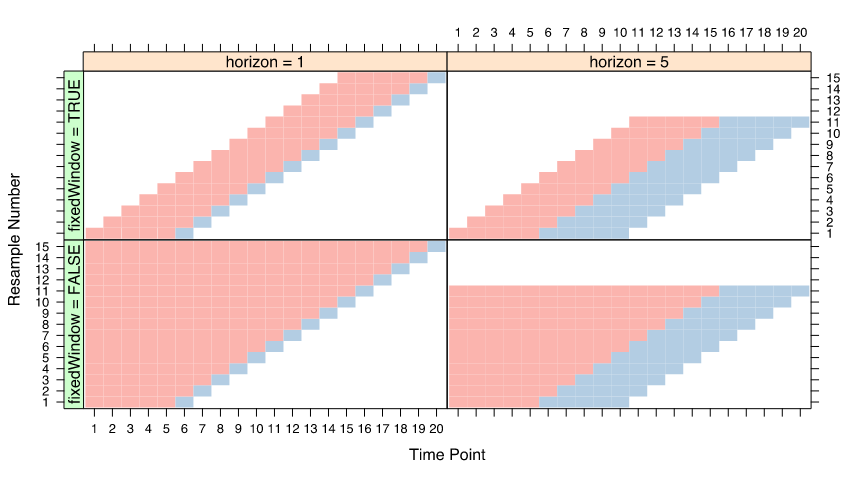
\includegraphics[width=\textwidth]{images/time-series.png}
    \caption{Aplicación de ''Rolling Forecasting Origin'' a una serie de 20 elementos con un tamaño inicial de cada serie de 5 elementos. Los elementos en rojo pertenecen a la serie de entrenamiento, los azules a la serie de pruebas. Imagen obtenida de \cite{web:caret}}
    \label{fig:models_time-series}
\end{figure}

\subsubsection*{Modelos ARIMA}

La implementación del modelo ARIMA, acrónimo del inglés Autoregressive Integrated 
Moving Average, y generalización del modelo ARMA, acrónimo del inglés
Autoregressive Moving Range; permite, mediante el uso de la variación y regresión
de los datos estadísticos, encontrar patrones en dichos datos para poder realizar
predicciones a futuro.

Este proceso se lleva a cabo mediante ajustar el modelo con una serie de datos
de entrenamiento, tras lo que se procede a comprobar si el modelo se ajusta de forma
correcta. Una vez ajustado y comprobado el modelo, este puede generar nuevas
predicciones.

\subsubsection*{Modelos STL con ETS\footnote{https://otexts.com/fpp2/weekly.html}}

También se ha implementado el modelo STL, acrónimo del inglés 
''Seasonal and Trend decomposition using Loess'', para descomponer las 
series temporales junto con el modelo ETS, acrónimo del inglés ''Error, Trend 
and Seasonal''.

Estos modelos obtienen predicciones de los datos ajustados estacionalmente mediante 
aplicar a estos predicciones no estacionales, y reajustando esa estacionalidad
usando los últimos datos de la serie de datos originales (ajustados estacionalmente).

\subsection{Modelos de Machine-Learning y Deep-Learning}

\subsubsection*{Modelos de Regresión Lineal}

Los modelos de Regresión Lineal utilizan las dos variables presentes en los datos,
en este caso, throughput y tiempo, para aproximar la relación de dependencia entre
ambas variables.

Una vez conocida la relación entre ambas variables, el modelo puede predecir futuros
valores en base a dicha relación.

\subsubsection*{Modelos Generalizados Aditivos}

Los Modelos Generalizados Aditivos son una extensión de los Modelos Lineales 
Generalizados, y consideran que la relación entre las variables respuesta (la variable
que queremos predecir, en este caso, el throughput) y las variables explicativas (la
variable que se utiliza para realizar las predicciones, en este caso, el tiempo) puede
tomar cualquier forma funcional, no únicamente lineal.

Mediante esta consideración, estos modelos toman los datos y realizan predicciones
mediante la aplicación de la relación entre ambas variables y las funciones que pueden
representar.

\subsubsection*{Modelos Generalizados Lineales}

Los Modelos Generalizados Lineales generalizan la Regresión Lineal permitiendo que
el modelo lineal se relacione con la variable de respuesta a través de una función
de enlace y permitiendo que la magnitud de la varianza de cada medida sea una función
de su valor predicho.

Esto permite al modelo realizar predicciones mediante aplicar los datos ya obtenidos
y la función de enlace, que depende de la distribución de los propios datos.

\subsubsection*{Modelos de ''Random Forest''}

Los modelos de ''Random Forest'' aplican los datos a un algoritmo de Machine-Learning 
que combina múltiples árboles de decisión clasificando y aplicando regresión a dichos
datos.

Este algoritmo se entrena aprendiendo a clasificar los datos obtenidos, de forma
que el ''random forest'' crece conforme aprende a clasificar nuevos elementos, de 
forma que con nuevos datos no clasificados, sea capaz de predecir su clasificación,
es decir, el algoritmo, una vez entrenado, será capaz de predecir el comportamiento
del sistema al clasificar los nuevos datos recibidos.

\subsubsection*{Modelos de Redes Neuronales}

De forma similar a los modelos de ''Random Forest'', los modelos de redes neuronales
utilizan los datos obtenidos para entrenar una red neuronal que, una vez entrenada,
podrá predecir el comportamiento del sistema mediante clasificar los nuevos valores.\\


De forma adicional, este programa permite aplicar la primera derivada previa aplicación 
de estos modelos predictivos, pudiendo obtener la pendiente de las predicciones 
realizadas.


%%%%%%%%%%%%%%%%%%%%%%%%%%%%%%%%%%%%%%%%%%%%%%%%%%%%%%%%%%%%%%%%%%%%%%%%%%%%%%%%
%%%%%%%%%%%%%%%%%%%%%%%%%%%%%%%%%%%%%%%%%%%%%%%%%%%%%%%%%%%%%%%%%%%%%%%%%%%%%%%%

\section{Resultados esperados} \label{sct:desarrollo_resultadosesperados}

En el momento de la escritura de este Trabajo de Fin de Grado, debido a 
problemas de tiempo, causados por retrasos en el desarrollo de pruebas y 
obtención de resultados previos, no se ha podido aplicar y probar estos
modelos de predicción.

A pesar de esto, al conocer el funcionamiento de estos modelos, se pueden
esperar ciertos resultados de la aplicación de los mismos a este trabajo.

Estos resultados esperados mostrarán una predicción del comportamiento del sistema
en base a los valores anteriores, generando una gráfica en la que se mostrarán
los datos anteriores junto con las predicciones de los modelos, generando un
gráfico similar al de la \autoref{fig:models_results}.

\begin{figure}[htpb]
    \centering
    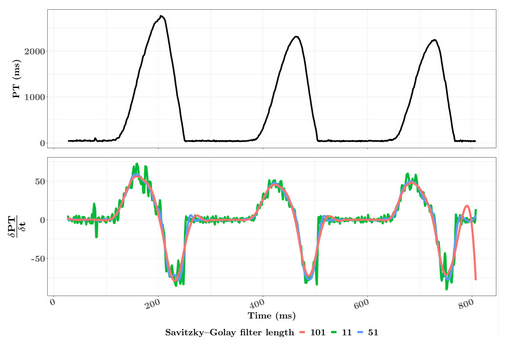
\includegraphics[width=0.5\textwidth]{images/ejemplo-res.png}
    \caption{Ejemplo de resultado de los modelos predictivos.}
    \label{fig:models_results}
\end{figure}
\chapter{Impacto del trabajo} \label{chp:impacto}

En este capítulo se hace un análisis del impacto general del trabajo 
desarrollado en este TFG, así como el impacto del mismo conforme a los 
Objetivos de Desarrollo Sostenible.

%%%%%%%%%%%%%%%%%%%%%%%%%%%%%%%%%%%%%%%%%%%%%%%%%%%%%%%%%%%%%%%%%%%%%%%%%%%%%%%%
%%%%%%%%%%%%%%%%%%%%%%%%%%%%%%%%%%%%%%%%%%%%%%%%%%%%%%%%%%%%%%%%%%%%%%%%%%%%%%%%

\section{Impacto general} \label{sct:impacto_impactogeneral}

Los sistemas distribuidos publicador/subscriptor se encuentran en una etapa de
grandes avances y desarrollos, pues son una tecnología ampliamente usada al 
vivir en un mundo cada día más digitalizado. 

De igual forma, la computación en la nube ha sufrido grandes avances, al 
proporcionar una plataforma en la que los usuarios pueden desplegar sus sistemas
y pagar solo por los recursos usados, a diferencia de la tradicional forma de 
desplegar sistemas de cara al público mediante tener recursos de computación 
estáticos, los cuales puedes estar desaprovechados y conllevan mayores costes.

Mediante el uso de computación en la nube y aplicando un buen sistema de 
auto-escalado, estos sistemas publicador/subscriptor proporcionarán un servicio
eficiente minimizando el coste de despliegue y mantenimiento.

En este proyecto, desde su inicio con la implementación del sistema
SilboPS\cite{thesis:tesisSVavassori} y siguiendo con la posterior mejora de 
este, que ha resultado en el sistema 
E-SilboPS\cite{tfm:victor2017}\cite{thesis:tesisVictor}, se ha desarrollado 
un sistema publicador/subscriptor que implemente, de forma óptima 
y eficiente, la función de auto-escalado, de forma que el sistema requiera
de mínima supervisión y cumpla con lo previamente mencionado.

Mediante el desarrollo de este proyecto se pretende contribuir al avance y 
mejora de los sistemas publicador/subscriptor por medio de auto-escalado 
eficiente, lo que lleva a proporcionar un mejor servicio a los usuarios de
estos sistemas, de forma que el tiempo de respuesta en el que reciben las
publicaciones sea mínimo, incluso en situaciones de mucho tráfico en el 
sistema, a la vez que se minimiza el uso de los recursos de computación,
reduciendo los costes y el malgasto energético al no desperdiciar dichos 
recursos.

El trabajo llevado a cabo en este TFG, que complementa el ya realizado en los 
trabajos previamente mencionados, mediante el estudio del comportamiento del
sistema frente a una situación que refleja una real, y los modelos de 
predicción, se pretende aplicar mejoras al auto-escalado de dicho sistema, 
aumentando su eficiencia. Este estudio se ha llevado a cabo sobre una
configuración básica 1-1-1, de forma que se identifique el punto de saturación
del sistemas bajo esta configuración, resultado el cual, mediante la aplicación
de modelos de predicción, permitirá la implementación de mejoras del auto-escalado.

Este trabajo ha permitido establecer las bases para el desarrollo de futuras 
mejoras del auto-escalado del sistema E-SilboPS, las cuales se podrán 
implementar en otros sistemas publicador/subscriptor del mismo tipo.

%%%%%%%%%%%%%%%%%%%%%%%%%%%%%%%%%%%%%%%%%%%%%%%%%%%%%%%%%%%%%%%%%%%%%%%%%%%%%%%%
%%%%%%%%%%%%%%%%%%%%%%%%%%%%%%%%%%%%%%%%%%%%%%%%%%%%%%%%%%%%%%%%%%%%%%%%%%%%%%%%

\section{Objetivos de Desarrollo Sostenible} \label{sct:impacto_ods}

% https://www.un.org/sustainabledevelopment/es/objetivos-de-desarrollo-sostenible/
% https://www.agenda2030.gob.es/objetivos/home.htm

El impacto de este trabajo sobre los 17 Objetivos de Desarrollo Sostenible 
aprobados en 2015 por los Estados Miembros de las Naciones Unidas como parte
de la Agenda 2030 para el Desarrollo Sostenible\cite{web:agenda2030}, que se 
pueden ver en la \autoref{fig:ods}, se alinea con
el \textbf{Objetivo 9. Industria, innovación e infraestructura},
el \textbf{Objetivo 11. Ciudades y Comunidades Sostenibles} y 
con el \textbf{Objetivo 12. Producción y Consumo Responsable}.

\begin{figure}[htpb]
    \centering
    
\includegraphics[width=0.75\textwidth]{images/ODS.png}
    \caption{Objetivos de Desarrollo Sostenible (\textit{ODS}). Imagen obtenida de \cite{web:agenda2030}.}
    \label{fig:ods}
\end{figure}

Los sistemas publicador/subscriptor, como el tratado en este trabajo, están 
en constante desarrollo e innovación, y son utilizados en multitud de ámbitos y
casos de uso en la vida cotidiana, por lo que sus constantes mejoras son vitales
para el funcionamiento óptimo de estos sistemas. De igual forma, estas mejoras 
conllevan un menos consumo eléctrico, al requerir de menos operaciones por cada
evento, o de desplegar un menor número de sistemas publicador/subscriptor si cada 
un puede con más carga.

A causa de esto, esta tecnología y este trabajo se alinean principalmente con el 
\textbf{Objetivo 9. Industria, innovación e infraestructura}, y de forma más 
precisa, con las metas \textbf{9.1}, al crear una infraestructura sostenible; 
\textbf{9.2} debido al constante desarrollo e innovación de la tecnología; y 
\textbf{9.4}, ya que el objetivo es modernizar los sistemas publicador/subscriptor 
y hacerlos maś eficientes.

De igual forma, se alinean, del \textbf{Objetivo 11. Ciudades y 
comunidades sostenibles}, con las metas \textbf{11.3} Urbanización inclusiva y 
sostenible, al desarrollar sistemas informáticos sostenibles 
medio-ambientalmente mediante la reducción del consumo energético de estos 
sistemas, ya sea por la mayor eficiencia de las operaciones del sistema o por
la eficiencia del sistema completo, requiriendo de menos sistemas de este tipo
al poder aumentar la carga de cada uno, requiriendo de menor número de sistemas 
desplegados.

Por último, este trabajo, al reducir el consumo energético de estos sistemas 
mediante aumentar la eficiencia, también están relacionadas con las metas del
\textbf{Objetivo 12. Producción y consumo responsables}, principalmente, con la
\textbf{12.A} Ciencia y Tecnología para Sostenibilidad, al desarrollar un sistema
que puede ser usado para impulsar la transformación digital y llevar esta 
tecnología a lugares poco digitalizados.

El impacto medioambiental del trabajo desarrollado en este TFG es mínimo, pero
una vez cumplido el objetivo último de este proyecto (maximizar la eficiencia 
del auto-escalado de los sistemas publicador/subscriptor basados en contenido
mediante E-SilboPS), si estas mejoras se implantasen de forma generalizada en 
la sociedad, junto con la constante digitalización de la vida cotidiana, 
se podría reducir la contaminación producida por estos sistemas en gran medida, 
al ser estos más eficientes.

De forma adicional, este proyecto tiene un potencial impacto en todas aquellas
áreas que se beneficiarían de una mayor sostenibilidad mediante la 
transformación digital resultante de implementar y usar este tipo de sistemas,
principalmente, en el Internet of Things y en Smart Cities.
\chapter{Resultados y conclusiones} \label{chp:resultados}

En este capítulo final, se presentarán los resultados de este trabajo, 
las conclusiones personales del autor y el trabajo futuro del proyecto.

%%%%%%%%%%%%%%%%%%%%%%%%%%%%%%%%%%%%%%%%%%%%%%%%%%%%%%%%%%%%%%%%%%%%%%%%%%%%%%%%
%%%%%%%%%%%%%%%%%%%%%%%%%%%%%%%%%%%%%%%%%%%%%%%%%%%%%%%%%%%%%%%%%%%%%%%%%%%%%%%%

\section{Resultados} \label{sct:resultados_resultados}

Los resultados obtenidos de este trabajo muestran que, mediante la aplicación 
de la carga de trabajo real obtenida y la aplicación de los modelos
predictivos, se pueden obtener mejoras en el proceso de auto-escalado.

De igual forma, se ha implementado y probado de forma satisfactoria el generador
de cargas de trabajo real, lo que permite que si en un futuro se dispone de 
alguna otra carga real que pudiese ser de utilidad. Esto se consigue mediante 
el cambio en la configuración a la sintaxis correspondiente de la nueva carga 
de trabajo.

Como se ha mencionado en la \autoref{sct:modelos_modelos-pred}, al no haber 
podido aplicar los modelos de predicción, no se han podido obtener los 
resultados esperados, pero los conocimientos adquiridos durante la realización
de este trabajo, permitirán aplicar estos modelos predictivos para aplicar las
mejoras necesarias al sistema.

En general, los resultados han sido positivos, a pesar de no haber tenido tiempo
suficiente para poder llevar a cabo todas las tareas que se habían planteado en
un principio, debido principalmente a retrasos generados por problemas durante
el desarrollo y el análisis de los datos del sistema.


%%%%%%%%%%%%%%%%%%%%%%%%%%%%%%%%%%%%%%%%%%%%%%%%%%%%%%%%%%%%%%%%%%%%%%%%%%%%%%%%
%%%%%%%%%%%%%%%%%%%%%%%%%%%%%%%%%%%%%%%%%%%%%%%%%%%%%%%%%%%%%%%%%%%%%%%%%%%%%%%%

\section{Conclusiones personales} \label{sct:resultados_conclusiones}

El desarrollo de este proyecto ha sido muy gratificante, tanto personalmente como
académicamente, y me ha permitido aprender y desarrollarme como estudiante, desde
leer y entender documentos científicos hasta desarrollar código de forma eficiente
y profesional, poniendo en práctica tanto conocimientos obtenidos durante el grado
como aquellos obtenidos durante el desarrollo de este TFG.

Personalmente, me ha gustado mucho poder conocer y participar en el desarrollo de
este proyecto tan ambicioso y llamativo, así como conocer el estado actual de las
tecnologías relacionadas, tanto directa como indirectamente. El futuro de este
proyecto y los posibles resultados que se pueden obtener me resultan muy interesantes
y emocionantes.


%%%%%%%%%%%%%%%%%%%%%%%%%%%%%%%%%%%%%%%%%%%%%%%%%%%%%%%%%%%%%%%%%%%%%%%%%%%%%%%%
%%%%%%%%%%%%%%%%%%%%%%%%%%%%%%%%%%%%%%%%%%%%%%%%%%%%%%%%%%%%%%%%%%%%%%%%%%%%%%%%

\section{Trabajo futuro} \label{sct:resultados_trabajofuturo}

% Aplicar más modelos de pred.
El trabajo futuro de este proyecto, principalmente, abarca la aplicación de los 
modelos de predicción, en concreto, el de una carga incremental (se incrementa 
la carga de permanente), una carga puntual (incremento puntual de la carga), y
el de una carga no predecible (la carga se genera de forma aleatoria, 
en base a ciertos parámetros). Tras aplicar estos modelos, se analizarán los
resultados obtenidos y se compararán con los resultados de los actuales modelos
estadísticos de predicción para ver si se producen mejores predicciones con
estos modelos predictivos.

% Implementación de las mejoras
Siguiendo la aplicación de los modelos predictivos, las mejoras que se 
identifiquen a partir de los resultados de estos serán otro de los trabajos a
realizar en un futuro.

% Dependencias y versiones
De forma adicional, sería recomendable revisar y actualizar los paquetes y 
dependencias del proyecto, de forma que haya estabilidad y uniformidad en las 
versiones usadas, y se disponga de las últimas actualizaciones y mejoras de las
herramientas usadas, además de prevenir posibles vulnerabilidades, como la 
recientemente vulnerabilidad de Log4J\cite{web:log4j}.

% Unificar proyectos y docu
Finalmente, otra de las tareas futuras es la de unificar el proyecto E-SilboPS 
en uno solo, al estar actualmente compuesto por dos proyectos, integrando ambos
en uno solo y resolviendo cualquier problema de compatibilidad o conflicto, de
forma que este sea más manejable y pueda documentarse de forma extensa en el
futuro.

\printbibliography[heading=bibintoc]

%%-----------------------------------------------
%% Anexos
\appendix
\clearpage
%\addcontentsline{toc}{chapter}{\annexname}
\renewcommand{\thesection}{\Alph{section}}

\chapter{Anexo} \label{chp:anexo}

A continuación se muestra el código, las figuras y las métricas de interés procedentes del
desarrollo de este proyecto\footnote{Se puede acceder a las trazas de las pruebas, 
código de los programas desarrollados, y cualquier recurso utilizado en este TFG bajo
petición al autor.}.

%%%%%%%%%%%%%%%%%%%%%%%%%%%%%%%%%%%%%%%%%%%%%%%%%%%%%%%%%%%%%%%%%%%%%%%%%%%%%%%%
%%%%%%%%%%%%%%%%%%%%%%%%%%%%%%%%%%%%%%%%%%%%%%%%%%%%%%%%%%%%%%%%%%%%%%%%%%%%%%%%

\section{Datos en crudo} \label{sct:anexo_datosencrudo}

\subsection*{Primeras 100 líneas de la traza resultante del generador}

\begin{lstlisting}[style=consola]
[
	{
		"eventType" : "S",
		"id" : "rmi://10.0.1.1:1099/Broker1-M23",
		"contextFunction" : {},
		"constraints" : {
			"class:str" : [{"=" : "broadcast"}]
		}
	},
	{
		"eventType" : "S",
		"id" : "rmi://10.0.1.1:1099/Broker1-M24",
		"contextFunction" : {},
		"constraints" : {
			"class:str" : [{"=" : "id7471312"}]
		}
	},
	{
		"eventType" : "P",
		"class:str" : "broadcast"
	},
	{
		"eventType" : "P",
		"class:str" : "broadcast"
	},
	{
		"eventType" : "P",
		"class:str" : "broadcast"
	},
	{
		"eventType" : "P",
		"class:str" : "broadcast"
	},
	{
		"eventType" : "P",
		"class:str" : "broadcast"
	},
	{
		"eventType" : "S",
		"id" : "rmi://10.0.1.1:1099/Broker1-M36",
		"contextFunction" : {},
		"constraints" : {
			"class:str" : [{"=" : "__announce__"}]
		}
	},
	{
		"eventType" : "P",
		"class:str" : "__announce__"
	},
	{
		"eventType" : "P",
		"class:str" : "id11296229"
	},
	{
		"eventType" : "P",
		"class:str" : "ProxyID_-3884500000",
		"x:str" : "0.0",
		"y:str" : "0.0"
	},
	{
		"eventType" : "P",
		"class:str" : "id11296229"
	},
	{
		"eventType" : "P",
		"class:str" : "id11296229"
	},
	{
		"eventType" : "P",
		"class:str" : "id11296229"
	},
	{
		"eventType" : "P",
		"class:str" : "__announce__"
	},
	{
		"eventType" : "P",
		"class:str" : "id11296229"
	},
	{
		"eventType" : "P",
		"class:str" : "id11296229"
	},
	{
		"eventType" : "P",
		"class:str" : "id11296229"
	},
	{
		"eventType" : "P",
		"class:str" : "id11296229"
	},
	{
		"eventType" : "P",
		"class:str" : "id11296229"
	},
	{
		"eventType" : "P",
		"class:str" : "id11296229"
	},
	{
\end{lstlisting}

\subsection*{Primeras 100 líneas de la traza resultante que conforma la \autoref{fig:subsworkload_th_fast_spike_25k-113k-100k}} \label{ssct:anexo_fast-spike}

\begin{lstlisting}[style=consola]
"timestamp","throughput"
30.414,100401
30.912,100401
31.419,98619
31.917,100401
32.414,100603
32.913,100200
33.412,100200
33.919,98619
34.412,101419
34.917,99009
35.473,89928
35.913,113636
36.413,100000
36.917,99206
37.417,100000
37.918,99800
38.417,100200
38.914,100603
39.416,99601
39.917,99800
40.416,100200
40.913,100603
41.417,99206
41.916,100200
42.416,100000
42.916,100000
43.416,100000
43.916,100000
44.415,100200
44.916,99800
45.412,100806
45.916,99206
46.416,100000
46.912,100806
47.436,95419
47.912,105042
48.416,99206
48.915,100200
49.416,99800
49.916,100000
50.416,100000
50.914,100401
51.416,99601
51.938,95785
52.415,104821
52.918,99403
53.416,100401
53.916,100000
54.417,99800
54.916,100200
55.415,100200
55.913,100401
56.412,100200
56.915,99403
57.415,100000
57.913,100401
58.417,99206
58.912,101010
59.414,99601
59.917,99403
60.416,100200
60.916,100000
61.415,100200
61.916,99800
62.415,100200
62.916,99800
63.416,100000
63.913,100603
64.417,99206
64.915,100401
65.416,99800
65.915,100200
66.416,99800
66.916,100000
67.417,99800
67.916,100200
68.416,100000
68.916,100000
69.416,100000
69.915,100200
70.416,99800
70.916,100000
71.416,100000
71.912,100806
72.416,99206
72.916,100000
73.412,100806
73.944,93984
74.417,105708
74.916,100200
75.414,100401
75.916,99601
76.416,100000
76.916,100000
77.416,100000
77.915,100200
78.416,99800
78.915,100200
79.412,100603
\end{lstlisting}


%%%%%%%%%%%%%%%%%%%%%%%%%%%%%%%%%%%%%%%%%%%%%%%%%%%%%%%%%%%%%%%%%%%%%%%%%%%%%%%%
%%%%%%%%%%%%%%%%%%%%%%%%%%%%%%%%%%%%%%%%%%%%%%%%%%%%%%%%%%%%%%%%%%%%%%%%%%%%%%%%

\section{Datos adicionales} \label{sct:anexo_datosadicionales}

\subsection*{Scripts en R}

\begin{lstlisting}[language=R, caption={Programa en R que genera una carga de subscripciones incremental, como en la \autoref{fig:subs_workload-growing}}]
library(ggplot2)
library(dplyr)
library(tikzDevice)

# Function to export plot to LaTeX
print_LaTeX_plot <- function(path, plot, width, height) {
  tikz(filename = path, standAlone = TRUE, width = width, height = height)
  print(plot)
  dev.off()
  tools::texi2pdf(path, quiet = TRUE)
}

export_plots = TRUE
setwd(dirname(rstudioapi::getActiveDocumentContext()$path))

OUTPUT_CSV_DIR = "path/for/csv"
OUTPUT_PLOT_DIR = "/paht/for/plot/pdf"
low_workload  = 50000 # Stable system
high_workload = 75000 # System saturates


amount_noise = 0

total_duration = 60
windows_per_second = 10
total_windows = total_duration * windows_per_second

chunk_size = total_windows / 10

# First chunk (low steady)
first_chunk <- data.frame(subscriptions = rep(low_workload, chunk_size))

# Second chunk (increase)
step = (high_workload - low_workload) / (chunk_size * 2)
second_chunk <- data.frame(subscriptions = seq(low_workload, high_workload, step))

# Last chunk (high steady)
last_chunk <- data.frame(subscriptions = rep(high_workload, chunk_size * 7))

# Combine all chunks
workload <- rbind(first_chunk, second_chunk, last_chunk)

# Add noise
x <- workload$subscriptions
corrupt <- rbinom(length(x), 1, 1)    # choose an average of 10% to corrupt at random
corrupt <- as.logical(corrupt)
noise <- rnorm(sum(corrupt), 0, amount_noise) # generate the noise to add
x[corrupt] <- x[corrupt] + noise      # about 10% of x has been corrupted
workload$subscriptions <- x

plot <- ggplot(workload, aes(x = c(1:nrow(workload)))) +
  geom_line(aes(y = subscriptions), size=1) +
  xlab("Tiempo (segundos)") +
  ylab("Subscripciones") +
  theme(legend.position = "bottom",
        legend.text = element_text(size = 18, face="bold"),
        legend.title = element_text(size = 18, face="bold"),
        axis.text.x = element_text(size = 18, face="bold"),
        axis.text.y = element_text(size = 18, face="bold"),
        axis.title.x = element_text(size = 18, face="bold"),
        axis.title.y = element_text(size = 18, face="bold"))
plot

print_LaTeX_plot(OUTPUT_PLOT_DIR, plot = plot, width = 10, height = 5)

# Export
workload <- as.integer(workload$subscriptions)
write.table(workload, OUTPUT_CSV_DIR, col.names = FALSE, row.names = FALSE, sep = ";")
\end{lstlisting}

\begin{lstlisting}[language=R, caption={Programa en R para obtener la carga representada en \autoref{fig:subs_workload-growing}}]
library(ggplot2)
library(tikzDevice)

# Function to export plot to LaTeX
print_LaTeX_plot <- function(path, plot, width, height) {
  tikz(filename = path, standAlone = TRUE, width = width, height = height)
  print(plot)
  dev.off()
  tools::texi2pdf(path, quiet = TRUE)
}
export_plots = TRUE
setwd(dirname(rstudioapi::getActiveDocumentContext()$path))

##### Datos del plot #####

FILE_PATH = "../../logs/reports"
FILE_NAME = "logs-subs-10reps.csv"
XLABEL = "Subscripciones"
YLABEL = "Throughput (notificaciones/s)"
THEME <- theme(legend.position = "bottom",
               legend.text  = element_text(size = 18, face="bold"),
               legend.title = element_text(size = 18, face="bold"),
               axis.text.x  = element_text(size = 18, face="bold"),
               axis.text.y  = element_text(size = 18, face="bold"),
               axis.title.x = element_text(size = 18, face="bold"),
               axis.title.y = element_text(size = 18, face="bold"))

##### Codigo generador del plot #####

data <- read.csv(paste(FILE_PATH, FILE_NAME, sep="/"), header = TRUE, sep = ",")

plot <- ggplot(data, aes(x = subscriptions)) +
  geom_line(aes(y = throughput), size=1) +
  xlab(XLABEL) +
  ylab(YLABEL) +
  scale_y_log10(breaks = c(1, 30000, 40000, 50000, 60000, 70000, 80000),
                     labels = c("1", "30k", "40k", "50k", "60k", "70k", "80k")) +
  scale_x_log10(breaks = c(1, 10,100, 1000, 100000),
                labels = c("1", "10", "100", "1k", "100k")) +
  

print_LaTeX_plot("./throughput_logsubs.tex", plot = plot, width = 10, height = 5)
\end{lstlisting}

\begin{lstlisting}[language=R, caption={Programa en R que genera una carga de subscripciones con un pico puntual, como en la \autoref{fig:subsworkload_20k-100k}}]
library(ggplot2)
library(dplyr)
library(tikzDevice)

# Function to export plot to LaTeX
print_LaTeX_plot <- function(path, plot, width, height) {
  tikz(filename = path, standAlone = TRUE, width = width, height = height)
  print(plot)
  dev.off()
  tools::texi2pdf(path, quiet = TRUE)
}

export_plots = TRUE
setwd(dirname(rstudioapi::getActiveDocumentContext()$path))


# SCRIPT PARAMETERS
OUTPUT_CSV_DIR = "path/for/csv"
OUTPUT_PLOT_DIR = "path/for/plot/pdf"
low_workload  = 25000  # Stable system
high_workload = 113904  # System saturates
fast_inc = TRUE
plain_spike = FALSE


amount_noise = 0

total_duration = 60
windows_per_second = 10
total_windows = total_duration * windows_per_second

chunk_size = total_windows / 10

# First chunk (low steady)
first_chunk <- data.frame(subscriptions = rep(low_workload, chunk_size*3))

# Second chunk (fast or slow increase)
step_up = (high_workload - low_workload) / ((chunk_size)*(fast_inc) ? 10 : 1)
second_chunk <- data.frame(subscriptions = seq(low_workload, high_workload, step_up))

if (plain_spike) {
  # Extra chunk (top steady)
  extra_chunk <- data.frame(subscriptions = rep(high_workload, chunk_size*0.5))
}

# Third chunk (decrease)
third_chunk <- data.frame(subscriptions = seq(high_workload, low_workload, -step_up))

# Last chunk (low steady)
last_chunk <- data.frame(subscriptions = rep(low_workload, chunk_size*3))

# Combine all chunks
if (plain_spike) {
  workload <- rbind(first_chunk, second_chunk, third_chunk, last_chunk)
}else {
  workload <- rbind(first_chunk, second_chunk, extra_chunk, third_chunk, last_chunk)
}

# Add noise
x <- workload$subscriptions
corrupt <- rbinom(length(x), 1, 1)    # choose an average of 10% to corrupt at random
corrupt <- as.logical(corrupt)
noise <- rnorm(sum(corrupt), 0, amount_noise) # generate the noise to add
x[corrupt] <- x[corrupt] + noise      # about 10% of x has been corrupted
workload$subscriptions <- x

plot <- ggplot(workload, aes(x = c(1:nrow(workload)))) +
  geom_line(aes(y = subscriptions), size=1) +
  xlab("Tiempo (segundos)") +
  ylab("Subscripciones") +
  theme(legend.position = "bottom",
        legend.text = element_text(size = 18, face="bold"),
        legend.title = element_text(size = 18, face="bold"),
        axis.text.x = element_text(size = 18, face="bold"),
        axis.text.y = element_text(size = 18, face="bold"),
        axis.title.x = element_text(size = 18, face="bold"),
        axis.title.y = element_text(size = 18, face="bold"))

plot

print_LaTeX_plot(OUTPUT_PLOT_DIR, plot = plot, width = 10, height = 5)

# Export
workload <- as.integer(workload$subscriptions)
write.table(
  workload,
  OUTPUT_CSV_DIR,
  col.names = FALSE,
  row.names = FALSE,
  sep = ";")
\end{lstlisting}

\begin{lstlisting}[language=R, caption={Programa en R para generar las gráficas del Throughput y del Tiempo de Respuesta.}]
library(ggplot2)
library(tikzDevice)

setwd(dirname(rstudioapi::getActiveDocumentContext()$path))


# Function to export plot to LaTeX
print_LaTeX_plot <- function(path, plot, width, height) {
  tikz(filename = path, standAlone = TRUE, width = width, height = height)
  print(plot)
  dev.off()
  tools::texi2pdf(path, quiet = TRUE)
}
export_plots = TRUE

##### Vars. and flag #####

# Paths of the dir with measurements and of each csv
DIR_PATH = "path/to/dir/of/measurements"
FILE_NAME_TH = "path/to/th.csv"
FILE_NAME_RT = "path/to/rt.csv"

# Specify plots
PLOT_TH = TRUE
PLOT_RT = TRUE

# Number of points on the plot
N_POINTS = 50

THEME <- theme(legend.position = "bottom",
               legend.text = element_text(size = 18, face="bold"),
               legend.title = element_text(size = 18, face="bold"),
               axis.text.x = element_text(size = 18, face="bold"),
               axis.text.y = element_text(size = 18, face="bold"),
               axis.title.x = element_text(size = 18, face="bold"),
               axis.title.y = element_text(size = 18, face="bold"))

##### THROUGHPUT #####

if (PLOT_TH) {

  # Name of plot labels and generated PDF
  OUT_FILE_TH = paste("./th_",FILE_NAME_TH,".tex", sep="")
  XLABEL_TH = "Tiempo (segundos)"
  YLABEL_TH = "Throughput (notifs/s)"

  data_th <- read.csv(paste(DIR_PATH, FILE_NAME_TH, sep="/"), header = TRUE, sep = ",")

  # Delete first values if needed (system not entirely up, so times are very high)
  data_th <- data_th[-c(0:3),]

  # Spit data frame in N_POINTS equal-sized data frames and find mean
  data_th$points <- cut(c(1:nrow(data_th)),
                        breaks=(nrow(data_th)/N_POINTS)*(0:N_POINTS),
                        labels=c(1:N_POINTS))

  # Mean for each point
  new_data_th <- aggregate(cbind(timestamp, throughput) ~ points,
                        data = data_th, FUN = mean, na.rm = TRUE)

  # To plot all points, replace 'new_data_th' with 'data_th'
  plot_th <- ggplot(data_th, aes(x = timestamp)) +
    geom_line(aes(y = throughput), size=1) +
    xlab(XLABEL_TH) +
    ylab(YLABEL_TH) +
    scale_y_log10() +
    THEME

  print_LaTeX_plot(OUT_FILE_TH, plot = plot_th, width = 10, height = 5)
}

##### RESPONSE TIME #####

if (PLOT_RT) {

  # Name of plot labels and generated PDF
  OUT_FILE_RT = paste("./rt_",FILE_NAME_RT,".tex", sep="")
  XLABEL_RT = "ID Notificacion"
  YLABEL_RT = "Tiempo de respuesta (segundos)"

  data_rt <- read.csv(paste(DIR_PATH, FILE_NAME_RT, sep="/"), header = TRUE, sep = ",")

  # Delete first values if needed (system not entirely up, so times are very high)
  data_rt <- data_rt[-c(0:1),]

  # Spit data frame in N_POINTS equal-sized data frames and find mean
  data_rt$points <- cut(c(1:nrow(data_rt)),
                        breaks=(nrow(data_rt)/N_POINTS)*(0:N_POINTS),
                        labels=c(1:N_POINTS))

  # Mean for each point
  new_data_rt <- aggregate(cbind(id, resp_time) ~ points,
                        data = data_rt,
                        FUN = mean,
                        na.rm = TRUE)

  plot_rt <- ggplot(data_rt, aes(x = id)) +
    geom_line(aes(y = resp_time), size=1) +
    xlab(XLABEL_RT) +
    ylab(YLABEL_RT) +
    THEME

  print_LaTeX_plot(OUT_FILE_RT, plot = plot_rt, width = 10, height = 5)
}

\end{lstlisting}

%%%%%%%%%%%%%%%%%%%%%%%%%%%%%%%%%%%%%%%%%%%%%%%%%%%%%%%%%%%%%%%%%%%%%%%%%%%%%%%%
%%%%%%%%%%%%%%%%%%%%%%%%%%%%%%%%%%%%%%%%%%%%%%%%%%%%%%%%%%%%%%%%%%%%%%%%%%%%%%%%

%%-----------------------------------------------
\end{document}
